% \documentclass{article}
% \documentclass[professionalfont,notes]{beamer}
\documentclass[professionalfont]{beamer}

%%%%%%%%%%%%%%%%%%%%%%%%%%%%%%%
%%% packages
\usepackage[utf8]{inputenc}
\usepackage[brazilian]{babel}
\usepackage{amssymb} %Mathematics
\usepackage{amsfonts}%Mathematics
\usepackage{amsmath,amscd}%Mathematics
\usepackage{amsthm}%Mathematics
\usepackage{mathrsfs}%Mathematics font
\usepackage{newtxtext,newtxmath}
\usepackage{xfrac}
\usepackage{cite}
\usepackage{ragged2e}
\usepackage{geometry}
\usepackage{calc}
\usepackage{graphicx}
\usepackage{tikz}
\usepackage{array}
\usepackage{tikz-3dplot}
\usepackage{tikz-dimline}
\usepackage{ragged2e}
\usepackage[absolute,overlay]{textpos} % para usar textblock
\usepackage{tcolorbox}
\usepackage[absolute,overlay]{textpos}
% \usepackage[font=small,compatibility=false]{caption}
\usepackage[font=footnotesize]{subcaption}
% \usepackage{subfig}
\usepackage{nicefrac}
% % tabelas
% \usepackage{tabularx,ltxtable} % also load longtable
% \usepackage{array,xparse}
%%%%%%%%%%%%%%%%%%%%%%%%%%%%%%%

%% tabelas
\usepackage{tabularx,ltxtable} % also load longtable
\usepackage{array,xparse}
% \usepackage{longtable}
\usepackage{makecell}
% \usepackage{hhline}
\usepackage{cellspace}
\usepackage{colortbl}

%%%%%%%%%%%%%%%%%%%%%%%%%%%%%%
%%%% definitions
\everymath{\displaystyle}
\usetheme{Warsaw}
%%%%%%%%%%%%%%%%%%%%%%%%%%%%%%

%%%%%%%%%%%%%%%%%%
% \setbeamertemplate{caption}[numbered]
% \setbeamertemplate{note page}[plain]
\setbeamertemplate{note page}[lookahead]
%%%%%%%%%%%%%%%%%%

%%%%%%%%%%%%%%%%%%%%%
% -- citacoes --
% \usepackage[brazilian,hyperpageref]{backref}	 % Paginas com as citações na bibl
\usepackage[alf,abnt-repeated-title-omit=yes,abnt-emphasize=bf,abnt-etal-list=0]{abntex2cite}
% \usepackage[alf,abnt-repeated-title-omit=yes,abnt-etal-list=0]{abntex2cite}
\citebrackets()
% -- citacoes --
%%%%%%%%%%%%%%%%%%%%%%

\newcommand{\dia}{\today}
\newcommand{\autor}{João Paulo Rodrigues de Andrade}
\newcommand{\orientador}{Darlan Karlo Elisiário de Carvalho}
\newcommand{\titulo}{Aplicação do método Multinível Algébrico Dinâmico Não Uniforme (NU-ADM) no escoamento composicional em reservatórios de petróleo.}
\newcommand{\instituicao}{Universidade Federal de Pernambuco}


%%%%%%%%%%%%%%%%%%%%%%%%%%%%%%%%%%%%%
%% novos comandos
\let\divsymb=\div % rename builtin command \div to \divsymb
\newcommand{\gv}[1]{\ensuremath{\mbox{\boldmath$ #1 $}}}
\renewcommand{\div}[1]{\gv{\vec{\nabla}} \cdot #1} % for divergence
\newcommand{\pd}[2]{\frac{\partial #1}{\partial #2}}
\newcommand{\grad}[1]{\gv{\nabla} #1} % for gradient
%%%%%%%%%%%%%%%%%%%%%%%%%%%%%%%%%%%%%


\def \porosidade{\phi}
\def \perm{K}
\def \poroVolume{V_{p}}
\def \totalVolume{V_{b}}
% \def \permTensor{\undertilde{K}}
\def \permTensor{\underline{\underline{K}}}
\def \Volume{V}
\def \velocity{\vec{v}}
\def \permRel{kr}
\def \phase{j}
\def \pressure{P}
\def \density{\rho}
\def \viscosity{\mu}
\def \milidarcy{md}
\def \gravity{g}
\def \permEff{k_{ef}}
\def \permAbs{K_{abs}}
\def \sourceTerm{Q}
\def \normalVec{\vec{n}}
\def \volumeSurface{\Gamma_{V}}
\def \faceVolume{L}
\def \normalVersor{\hat{n}} %remover
\def \Area{A}
\def \component{k}
\def \molNumber{n}
\def \molNumberComponent{\molNumber_{\component}} %remover
\def \globalMolarFraction{z}
\def \timme{t}
\def \bulkVolume{V_{b}}
\def \numberOfPhases{N_{\phase}}
\def \numberOfComponents{N_{c}}
\def \molarPartialFrac{x}
\def \altura{D}
\def \molarDensity{\xi}
\def \molarDensityPhase{\xi_{\phase}} %remover
\def \molarDensityComponent{\molarDensity_{\component}}  %remover
\def \mSourceTerm{q}
\def \totalFluidVolume{V_{t}}
\def \porosidadeIni{\porosidade^{0}}
\def \rockCompress{c_{f}}
\def \pressureIni{\pressure_{f}}
\def \aComponent{a_{\component}} %remover
\def \aPhase{a_{\phase}} % remover
\def \alphaComponent{\alpha_{\component}} %remover
\def \bComponent{b_{\component}} %remover
\def \bPhase{b_{\phase}} %remover
\def \componentt{\component_{1}} %%remover
\def \componenttt{\component_{2}} %%remover
\def \molarVolume{v}
\def \molarphaseVolume{\molarVolume_{\phase}} %remover
\def \molarVolumeComponent{\molarVolume_{\component}}  %remover
\def \rConstant{R}
\def \temperature{T}
\def \Joule{J}
\def \mol{mol}
\def \m3{m^{3}}
\def \binaryInter{\kappa}
\def \omegaA{\Omega_{a}} %remover
\def \omegaB{\Omega_{b}} %remover
\def \Critical{c}
\def \criticalT{\temperature_{\Critical}}
\def \criticalTComponent{\temperature_{\Critical \component}} %% remover
\def \criticalP{\pressure_{\Critical}}
\def \criticalPComponent{\pressure_{\Critical \component}} %remover
\def \criticalV{\Volume_{\Critical}}
\def \crititicalVComponent{\Volume_{\Critical \component}} %remover
\def \criticalMolarDensity{\molarDensity_{\Critical}}
\def \criticalMolarDensityPhase{\molarDensity_{\Critical \phase}} %remover
\def \malphaComp{\gamma_{\component}} %remover
\def \acentricFator{\omega}
\def \acentricFatorComponent{\acentricFator_{\component}}
\def \Zfactor{Z}
\def \ZfactorPhase{\Zfactor_{\phase}} % remover
\def \BPhase{B_{\phase}} %remover
\def \APhase{A_{\phase}} % remover
\def \fugacity{f_{\component \phase}}
\def \coefFugacity{\varphi}
\def \Saturation{S}
\def \oilPhase{o} % remover
\def \waterPhase{w} %remover
\def \gasPhase{g} %remover
\def \MolecularWeight{W}
\def \MolecularWeightComponent{\MolecularWeight_{\component}} % remover
\def \MolecularWeightPhase{\MolecularWeight_{\phase}} %remover
\def \viscosityComponent{\viscosity_{\component}} %remover
\def \viscosityLowPressure{\viscosity^{*}}
\def \viscosityLowPressureComponent{\viscosityLowPressure_{\component}} %remover
\def \Reduced{r} %remover
\def \reducedTemperature{\temperature_{\Reduced}}
\def \reducedTemperatureComponent{\temperature_{\Reduced \component}}%remover
\def \reducedPressure{\pressure_{\Reduced}}
\def \reducedMolarDensity{\molarDensity_{\Reduced}}
\def \zetaParam{\zeta}
\def \zetaParamComponent{\zetaParam_{\component}}
\def \atmPressure{atm}
\def \kelvinTemperature{K}
\def \reducedMolarDensity{\molarDensity_{\Reduced}}
\def \reducedMolarDensityPhase{\molarDensity_{\Reduced \phase}}
\def \etaParam{\eta}
\def \sumInComponents{\displaystyle \sum_{\component}^{\numberOfComponents}} %remover
\def \MolarMass{M}
\def \MolarMassComponet{\MolarMass_{\component}} %remover
\def \mobility{\lambda}
\def \mobilityPhase{\mobility_{\phase}} % remover
\def \totalMobility{\mobility_{T}}

\def \coarseRatio{Cr}
\def \volf {\Omega_{i}}
\def \volfBoundary{\partial \volf}
\def \volcoarse {\Omega_{I}}
\def \volDual{\Omega_{I}^{d}}
\def \boundaryVolDual{\partial \volDual}
\def \prolOperator{\underline{\underline{OP}}}
\def \level{l}
\def \prolOperatorIi{\prolOperator^{\level}_{\level-1}}
\def \restOperator{\underline{\underline{OR}}}
\def \restOperatorIi{\restOperator^{\level-1}_{\level}}
\def \basisFunction{\phi}
\def \basisFunctionIi{\basisFunction^{I}_{i}}
\def \correctionFunc{\phi^{*}}
\def \kroneckerDelta{\delta}
\def \correctionFunci{\correctionFunc_{i}}
\def \fine{f}
\def \vectorPressure{\mathbf{\pressure}^{\fine}}
\def \vectorFinePressureWire{\bold{P}^{fw}}

\def \msPressure{\pressure'}
\def \vectorMsPressure{\bold{\pressure}'}

\def \numberFineVols{N^{f}}
\def \numberCoarseVols{N^{c}}
\def \coarsePressure{\pressure_{I}^{c}}
\def \vectorCoarsePressure{\bold{\pressure}^{c}}
\def \permutationMatrix{\underline{\underline{G}}}
\def \transmissibility{T}
\def \fineTransmissibility{\underline{\underline{\transmissibility}}^{f}}
\def \vectorfineSource{\mathbf{q}^{f}}
\def \dualInternal{i}
\def \dualFace{f}
\def \dualEdge{e}
\def \dualVertex{v}
\def \finewirebasketMatrix{\underline{\underline{M}}}
\def \MIntInt{M_{\dualInternal \dualInternal}}
\def \MIntFac{M_{\dualInternal \dualFace}}
\def \MFacInt{M_{\dualFace \dualInternal}}
\def \MFacFac{M_{\dualFace \dualFace}}
\def \MFacEdg{M_{\dualFace \dualEdge}}
\def \MEdgFac{M_{\dualEdge \dualFace}}
\def \MEdgEdg{M_{\dualEdge \dualEdge}}
\def \MEdgVer{M_{\dualEdge \dualVertex}}
\def \MVertEdg{M_{\dualVertex \dualEdge}}
\def \MVertVert{M_{\dualVertex \dualVertex}}
\def \fineWirebasketSource{b}
\def \vectorFineWirebasketSource{\bold{b}}
\def \vectorFineWirebasketSourceMod{\bold{b}'}
\def \finewirebasketMatrixMod{\underline{\underline{{\tilde{M}}}}}
\def \MFacFacMod{\tilde{M}_{\dualFace \dualFace}}
\def \MEdgEdgMod{\tilde{M}_{\dualEdge \dualEdge}}
\def \coarseTransmissibility{\underline{\underline{\transmissibility}}^{c}}
\def \correctionFunctionMatrix{\underline{\underline{C}}}
\def \coarseSourceTerm{\bold{R}^{c}}
\def \identityMatrixVert{I_{\dualVertex \dualVertex}}
\def \spaceum{\hspace{0.1cm}}
\def \refFigura{Figura}
\def \vectorIntermPressure{\bold{P}''}
\def \IntermPressure{P''}
\def \prolOperatorAdm{\hat{\prolOperator}}
\def \restOperatorAdm{\hat{\restOperator}}
\def \vectorPressureAdm{\bold{\pressure}^{ADM}}

\def \permeability{K}
\def \molarPhaseFraction{\Upsilon}


\title[NU-ADM]{Aplicação do método Multinível Algébrico Dinâmico Não Uniforme (NU-ADM) no escoamento composicional em reservatórios de petróleo}
\author[João Paulo Rodrigues de Andrade]{João Paulo Rodrigues de Andrade}
\institute[UFPE]{Universidade Federal de Pernambuco}
% \titlegraphic{
\includegraphics[scale=0.2]{./imgs/ufpe.png} \hspace{0.5cm} 
\includegraphics[scale=0.2]{./imgs/ufpe.png}}

\date{}

\newcommand\Wider[2][3em]{%
\makebox[\linewidth][c]{%
  \begin{minipage}{\dimexpr\textwidth+#1\relax}
  \raggedright#2
  \end{minipage}%
  }%
}

%%%%%%%%%%%%%%%%%%%
%% tikz
\usetikzlibrary{matrix}
\usetikzlibrary{calc,3d}
\usetikzlibrary{arrows,positioning}
\usetikzlibrary{shapes.callouts}
\usetikzlibrary{shapes.geometric}
\usetikzlibrary{decorations.text}
\usetikzlibrary{math}
%%%%%%%%%%%%%%%%%%%


\setbeamersize{text margin left=0.5cm,text margin right=0.5cm}
\newlength\MyColSep
\setlength\MyColSep{1cm}
\newlength\MyColWd
\setlength\MyColWd{.5\textwidth}


\setbeamertemplate{sidebar right}{}
\setbeamertemplate{footline}{%
\hfill\usebeamertemplate***{navigation symbols}
\hspace{1cm}\insertframenumber{}/\inserttotalframenumber}


\begin{document}

% {
% \setbeamertemplate{background}{%
%   \raisebox{-1cm}{%
%     \parbox[c]{3cm}{\centering%
%       
\includegraphics[width=2cm]{./imgs/ufpe.png}%
%     }%
%     \parbox[c]{\dimexpr\paperwidth-3cm\relax}{\centering%
%       {\Large The Name of the University}%
%     }%
%   }%
% }

\begin{frame}
    % \titlepage
    \begin{minipage}{\textwidth}
    
    \begin{textblock*}{5cm}(0.5cm,2.3cm) % {block width} (coords)
        
\includegraphics[scale=0.2]{./imgs/ufpe.png}
    \end{textblock*}
    
    \begin{textblock*}{8cm}(2.3cm,3.5cm) % {block width} (coords)
        \Large \instituicao
    \end{textblock*}
    
    \begin{textblock*}{5cm}(10.5cm,2.4cm) % {block width} (coords)
        
\includegraphics[scale=0.25]{./imgs/padmec.jpeg}
    \end{textblock*}
    \end{minipage}
    
    \vspace{1.8cm}
    
    \begin{minipage}{\textwidth}
        \begin{tcolorbox}[halign=center,
    valign=center,colupper=black,boxsep=1pt,width=\textwidth,colback={white},colbacktitle=yellow]    
            \Large \titulo
        \end{tcolorbox}
    \end{minipage}
    
    \vspace{0.3cm}
    
    \begin{minipage}{\textwidth}
        \autor
        
        Orientador: \orientador
    \end{minipage}
    
    \vfill
        
    Recife, 03 de Novembro de 2022.
    
    % João Paulo Rodrigues de Andrade
    
    % Orientador: Darlan Karlo Elisiário de Carvalho
    
    % Recife, \today
    
\end{frame}

\begin{frame}{Sumário}
\begin{columns}[t]
        \begin{column}{.4\textwidth}
            \tableofcontents[sections={1-3}]
        \end{column}
        \begin{column}{.4\textwidth}
            \tableofcontents[sections={4-6}]
        \end{column}
    \end{columns}
\end{frame}

\section{Introdução}



\begin{frame}
\frametitle{Introdução}
\index{Introdução}
\begin{itemize}
    \item<1-> Importância da simulação computacional \note[item]{\scriptsize  a exploração de petróleo e gás é uma atividade que envolve a captação
    de grandes investimentos com altos riscos financeiros, por isso é essencial poder predizer o
    comportamento de um campo ou reservatório, por meio da simulação numérica. Um simulador numérico permite obter informações sobre o desempenho de um campo ou reservatório submetidos a vários cenários de produção, possibilitando encontrar  condições ótimas para se extrair petróleo desse campo}
    \item<2-> Importância da utilização de modelos composicionais \note[item]{
        \scriptsize Pode-se dizer que a recuperação de hidrocarbonetos em meios porosos ocorre em 3 fases: recuperação primária, secundária e terciária. Na recuperação primária, o reservatório tem a energia necessária para impulsionar o fluido para a superfície naturalmente. Na recuperação
    secundária, quando a pressão no reservatório não é suficiente para manter a produção, se faz necessário injetar outro fluido para aumentar a pressão, varrendo o óleo na direção dos poços produtores. Já nos métodos de recuperação terciária, ou avançada (\textit{Enhanced Oil Recovery - EOR}), o deslocamento do óleo ocorre pela redução da sua viscosidade, das forças capilares  ou da tensão superficial, sendo classificados em quatro categorias: químicos, miscíveis, térmicos e microbiológicos. Devido a complexidade desses métodos, se faz  necessária a aplicação de modelos mais acurados de simulação como o composicional, que consiste na modelagem do transporte dos componentes pelas fases.}
    \item<3-> Problema do tempo de simulação
    \item<4-> Métodos de Transferência de escala: \textit{Upscaling}, Multiescala, ADM (\textit{Algebraic Dynamic Multilevel Method})
    \item<5-> Método NU-ADM (\textit{Non Uniform Algebraic Dynamic Multilevel Method})
\end{itemize}
\end{frame}

% \subsection{Específicos}
% \begin{frame}{Objetivos}
    
%     \begin{block}{Específicos}
%         \begin{itemize}
%             \item Desenvolver um interpretador os dados do reservatório
%             \item Aplicar o método NU-ADM no modelo composicional IMPEC
%             \item Comparar a solução da malha fina com a obtida por meio do método NU-ADM
%         \end{itemize}
%     \end{block}
    
% \end{frame}

\section{Fundamentação Teórica}
% \begin{frame}{Lei de Darcy}

% \begin{textblock*}{.5\paperwidth}(0.2cm,2.7cm)
%     \centering
%     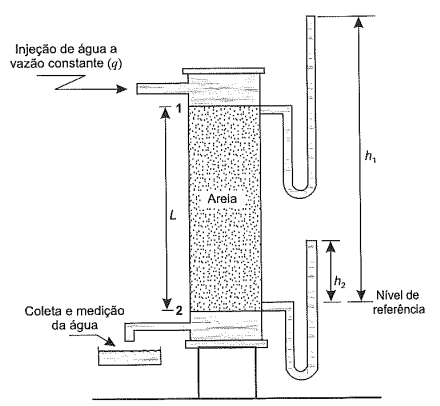
\includegraphics[scale=0.4]{./imgs/im1.png}
%     \footnotesize Retirado de \cite{Rosa2006}.
% \end{textblock*}

% \begin{textblock*}{.48\paperwidth}(6.4cm,3cm)
%     Darcy estabeleceu que, para qualquer vazão, a velocidade do fluxo é diretamente proporcional à diferença nas alturas manométricas \cite{044441830X}.
%     \begin{equation}
%         v = \perm \dfrac{h_{1} - h_{2}}{L}
%     \end{equation}
    
    
% \end{textblock*}

% \end{frame}

\subsection{Método dos volumes finitos}
% \begin{frame}{Método dos volumes finitos}
% \begin{figure}[!ht]
% \centering
%     \caption{Exemplos de malhas computacionais}
%     \begin{subfigure}[t]{.45\textwidth}
%         \centering
%         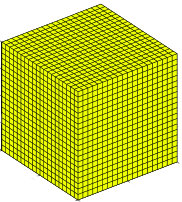
\includegraphics[scale=0.25]{./imgs/im3.png}
%         \caption{3D estruturada}
%         \label{fig:volumes_finitos1.a}
%     \end{subfigure}
%     \begin{subfigure}[t]{.45\textwidth}
%         \centering
%         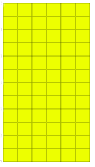
\includegraphics[scale=0.25]{./imgs/im4.png}
%         \caption{2D estruturada}
%         \label{fig:volumes_finitos1.b}
%     \end{subfigure}
%     \\
%     \begin{subfigure}{.45\textwidth}
%         \centering
%         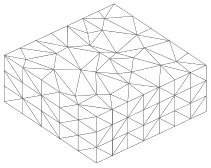
\includegraphics[scale=0.27]{./imgs/im6.png}
%         \caption{3D não estruturada}
%         \label{fig:volumes_finitos1.c}
%     \end{subfigure}
%     \begin{subfigure}{.45\textwidth}
%         \centering
%         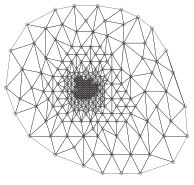
\includegraphics[scale=0.27]{./imgs/im5.png}
%         \caption{2D não estruturada}
%         \label{fig:volumes_finitos1.d}
%     \end{subfigure}

%     {\footnotesize Retirado de \cite{Knut2019}}
% \end{figure}

% \end{frame}

\begin{frame}{Método dos volumes finitos}

\begin{columns}
\begin{column}{0.6\textwidth}
% Equação do balanço de massa na forma integral:
Balanço de massa:
  \begin{equation}
	\label{eq:volumes_finitos.1}
	\int_{V} \pd{\rho}{t} dV = \int_{V} - \div{(\rho \velocity)} dV + \int_{V} Q dV
\end{equation}

% Aplicando o teorema da divergência de Gauss na segunda integral de \eqref{eq:volumes_finitos.1} \cite{Souza2015}:

Teorema da divergência de Gauss:

 \begin{equation}
	 \label{eq:volumes_finitos.2}
	 \int_{V} - \div{(\rho \velocity)} dV = \int_{\volumeSurface} - \rho \velocity \cdot \normalVec \text{ } d \volumeSurface
 \end{equation}

\end{column}
\begin{column}{0.4\textwidth}  %%<--- here
    \begin{equation}
        \fineTransmissibility \vectorPressure = \vectorfineSource
    \end{equation}

    \begin{description}[]
        \small
        \item $\volumeSurface$: contorno do volume $V$;
        \item $\rho$: densidade do fluido;
        \item $Q$: termo fonte ou sumidouro;
        \item $t$: tempo;
        \item $\fineTransmissibility$: matriz transmissibilidade;
        \item $\vectorPressure$: vetor de pressão;
        \item $\vectorfineSource$: vetor do termo fonte;
        \item $^{f}$: Malha fina
    \end{description}
    
\end{column}
\end{columns}

\end{frame}

\subsection{Lei de Darcy}
\begin{frame}{Lei de Darcy}
    % Generalizando:
    \begin{equation}
        \velocity = -\permTensor \dfrac{1}{\mu} (\grad{p} - \grad{D})
    \end{equation}
    
    \vspace{0.3cm}
    
    \begin{description}[]
        \item $\permTensor$ : tensor permeabilidade da rocha;
        \item $\velocity$: velocidade do fluido;
        \item $p$: pressão do fluido;
        \item $\mu$: viscosidade do fluido;
        \item $D$: altura do fluido
    \end{description}
    
    \begin{textblock*}{.5\paperwidth}(6cm,5cm)
        \begin{align*}
            \permTensor = 
            \begin{bmatrix}
            	K_{xx} & K_{xy} & K_{xz} \\
            	K_{yx} & K_{yy} & K_{yz} \\
            	K_{zx} & K_{zy} & K_{zz}
	        \end{bmatrix}
        \end{align*}
    \end{textblock*}
    
\end{frame}



\subsection{Modelo Composicional}

\begin{frame}{Simplificações}
    \begin{itemize}
        \item Escoamento isotérmico;
        % \item Equilíbrio termodinâmico local entre as fases;
        % \item Ausência do termo de pressão capilar;
        % \item Ausência do termo de gravidade;
        \item Ausência dos termos de pressão capilar e gravidade.
        \item A velocidade é dada pela Lei de Darcy;
        \item A água é imiscível e sua viscosidade é constante;
        \item O meio está totalmente saturado;
        % \item Rocha pouco compressível;
        % \item Não há reacão química entre os fluidos;
        \item Não há interação entre rocha e fluido, fenômeno de dispersão e reação química;
        % \item Não há o fenômeno de dispersão;
        % \item A viscosidade da fase água é constante;
        \item São consideradas 3 fases: água, óleo e gás.
    \end{itemize}
    
\end{frame}

\begin{frame}{Equações de estado}

% \begin{columns}
%     \begin{column}{0.6\textwidth}


%     \end{column}
%     \begin{column}{0.4\textwidth}  %%<--- here
%     \end{column}
% \end{columns}
    
    % Nesse trabalho foi utilizada a equação de Peng-Robinson dada por \cite{Chen2007}:
    Equação de Peng-Robinson:

    \begin{equation}
        \label{eq:eos.1}
        \pressure_{\phase} = \dfrac{\rConstant \temperature}{\molarphaseVolume - \bPhase} - \dfrac{\aPhase}{\molarphaseVolume(\molarphaseVolume + \bPhase) + \bPhase(\molarphaseVolume - \bPhase)}
    \end{equation}
    \begin{columns}
        \begin{column}{0.6\textwidth}
            \begin{description}[]
                \item $R$ constante dos gases ideais;
                \item $T$: temperatura;
                \item $\molarphaseVolume$: volume molar;
                \item $\aPhase, \bPhase$: variáveis empíricas da equação
                \item $_{j}$: fase
            \end{description}
        \end{column}
    \end{columns}
    
\end{frame}

% \begin{frame}{Equações de estado}

%     Sabendo que $\ZfactorPhase = \dfrac{\pressure_{\phase} \molarphaseVolume}{\rConstant \temperature}$, substituindo em \eqref{eq:eos.1} e fazendo as devidas manipulações, chega-se a equação cúbica para $\ZfactorPhase$:

%     \begin{equation}
%         \label{eq:eos.8}
%         \ZfactorPhase^{3} - (1 - \BPhase) \ZfactorPhase^{2} + (\APhase - 2 \BPhase - 3 \BPhase^{2}) \ZfactorPhase - (\APhase \BPhase - \BPhase^{2} - \BPhase^{3}) = 0,
%     \end{equation}

%     sendo:

%     \begin{equation}
%         \label{eq:eos.9}
%         \APhase = \dfrac{\aPhase \pressure_{\phase}}{\rConstant^{2} \temperature^{2}}, \hspace{1cm} \BPhase = \dfrac{\bPhase \pressure_{\phase}}{\rConstant \temperature}, 
%     \end{equation}

%     e $\ZfactorPhase$ o fator de compressibilidade do fluido. O método de solução das raízes de \eqref{eq:eos.9} pode ser encontrado em \cite{Chen2007,Chen2006,Soprano_2013}.

% \end{frame}

% \begin{frame}{Equações de estado}
%     Fugacidade: é uma medida da quantidade que um fluido desvia-se do comportamento do gás ideal, dada por:

%     \begin{equation}
%         \label{eq:eos.11}
%         \fugacity = \pressure_{\phase} \molarPartialFrac_{\component \phase} \coefFugacity_{\component \phase}, \hspace{0.7cm} \component=1,...,\numberOfComponents, \hspace{0.7cm} j = o,g ,
%     \end{equation}

%     \begin{description}[]
%         \item $\molarPartialFrac_{\component \phase}$: fração molar do componente ($\component$) na fase ($\phase$);
%         \item  $\coefFugacity_{\component \phase}$: coeficiente de fugacidade do componente $\component$ na fase $\phase$;
%         \item $\fugacity$: fugacidade do componente $\component$ na fase $\phase$;
%         \item $\numberOfComponents$: número de componentes
%     \end{description}
    
% \end{frame}

% \begin{frame}{Equações de Estado}
%     Onde $\coefFugacity_{\component \phase}$ pode ser encontrado por

%     \begin{equation}
%         \small
%         \label{eq:eos.10}
%         \begin{aligned}
%             &\ln (\coefFugacity_{\componentt \phase}) = \dfrac{b_{\componentt}}{\bPhase} (\ZfactorPhase - 1) - \ln (\ZfactorPhase - \BPhase)\\
%             &- \dfrac{\APhase}{2\sqrt{2} \BPhase} \left(\dfrac{2}{\aPhase} \sum_{\componenttt}^{\numberOfComponents} \molarPartialFrac_{\componenttt \phase}(1 - \binaryInter_{\componentt \componenttt})\sqrt{a_{\componentt} a_{\componenttt}} - \dfrac{b_{\componentt}}{\bPhase} \right) \ln \left(\dfrac{\ZfactorPhase + \left[1 + \sqrt{2} \right] \BPhase}{\ZfactorPhase - \left[1 - \sqrt{2} \right] \BPhase} \right),
%         \end{aligned}
%     \end{equation}

%     Sendo $\binaryInter_{\componentt \componenttt}$ o coeficiente de interação binária entre os componentes $\componentt$ e $\componenttt$.

% \end{frame}

% \begin{frame}{Cálculo de Estabilidade e Flash}

%     \begin{itemize}
%         \item O objetivo do cálculo de estabilidade é verificar se, dada as propriedades do fluido, ele vai se dividir em duas fases (óleo e gás) ou vai permancer numa fase apenas;
%         \item Caso o fluido se divida em duas fases, no cálculo de flash são encontrados os valores de frações molares dos componentes em cada fase e os respectivos valores de frações molares das fases óleo é gás, utilizando o procedimento de \citeonline{Rachford_1952}.
%     \end{itemize} 
    
% \end{frame}

% \begin{frame}{Equação da pressão}
%     Equação do balanço molar \cite{Fernandes_2014}:

%     \begin{equation}
%         \label{eq:modelo_mat.1}
%         \dfrac{1}{\bulkVolume} \pd{\molNumber_{\component}}{t} = \sum_{\phase}^{\numberOfPhases} \div{\left(\molarPartialFrac_{\component \phase} \molarDensityPhase \velocity_{\phase} \right)} + \dfrac{\mSourceTerm_{\component}}{\bulkVolume} ,
%     \end{equation}

%     \begin{description}[]
%         \item $\molNumber_{\component}$ = número de mols do componente $\component$;
%         \item $\molarDensityPhase \left[ \dfrac{mol}{\m3} \right]$ = densidade molar da fase $\phase$;
%         \item $\mSourceTerm_{\component} \left[ \dfrac{mol}{s} \right]$ = termo fonte do componente $\component$;
%         \item $\numberOfPhases$ = número de fases;
%         \item $\bulkVolume$ = Volume total
%     \end{description}
% \end{frame}

% \begin{frame}{Equação da pressão}
%     A equação da pressão é obtida igualando o volume poroso ao volume do fluido
%     \cite{Acs_1985}:

%     \begin{equation}
%         \label{eq:modelo_mat.2}
%         \poroVolume (\pressure) = \totalFluidVolume (\pressure, \molNumber_{1}, \molNumber_{2}, ..., \molNumber_{\numberOfComponents + 1}),
%     \end{equation}

%     \begin{description}[]
%         \item $\poroVolume$ = volume poroso = $\porosidade \bulkVolume$;
%         \item $\porosidade$ = porosidade = $\porosidadeIni \left[1 + \rockCompress (\pressure - \pressureIni) \right]$;
%         \item $\totalFluidVolume$ = volume total do fluido 
%         \item $\rockCompress$ = compressibilidade da rocha;
%         \item $\porosidadeIni$ = porosidade na pressão de referência $\pressureIni$
%     \end{description}
    
% \end{frame}

% \begin{frame}{Equação da pressão}
%     Derivando \eqref{eq:modelo_mat.2} com relação ao tempo:

%     \begin{equation}
%         \label{eq:modelo_mat.2.1}
%         \pd{\poroVolume}{\pressure} \pd{\pressure}{\timme} = \pd{\totalFluidVolume}{\pressure} \pd{\pressure}{\timme} + \sum_{\component}^{\numberOfComponents + 1} \left( \pd{\totalFluidVolume}{\molNumber_{\component}}  \right)_{\pressure} \pd{\molNumber_{\component}}{\timme}.
%     \end{equation}

%     Derivando o volume poroso em relação a pressão:

%     \begin{equation}
%         \label{eq:modelo_mat.5}
%         \pd{\poroVolume}{\pressure} = \bulkVolume \porosidadeIni \rockCompress .
%     \end{equation}
    
% \end{frame}

% \begin{frame}{Equação da pressão}
%     Substituindo \eqref{eq:modelo_mat.5} em \eqref{eq:modelo_mat.2} temos:

%     \begin{equation}
%         \label{eq:modelo_mat.6}
%         \bulkVolume \porosidadeIni \rockCompress \pd{\pressure}{\timme} = \pd{\totalFluidVolume}{\pressure} \pd{\pressure}{\timme} + \sum_{\component}^{\numberOfComponents + 1} \left( \pd{\totalFluidVolume}{\molNumber_{\component}}  \right)_{\pressure} \pd{\molNumber_{\component}}{\timme},
%     \end{equation}

%     Substituindo $\pd{\molNumber_{\component}}{\timme}$ de \eqref{eq:modelo_mat.6} em  \eqref{eq:modelo_mat.1} temos a equação da pressão:

%     \begin{equation}
%         \label{eq:modelo_mat.7}
%         \left( \porosidadeIni \rockCompress - \dfrac{1}{\bulkVolume} \pd{\totalFluidVolume}{\pressure} \right) \pd{\pressure}{\timme} = \sum_{\component}^{\numberOfComponents + 1} \left( \pd{\totalFluidVolume}{\molNumber_{\component}}  \right)_{\pressure} \left[ \sum_{\phase}^{\numberOfPhases} \div{\left(\molarPartialFrac_{\component \phase} \molarDensityPhase \velocity_{\phase} \right)} + \dfrac{\mSourceTerm_{\component}}{\bulkVolume}\right], 
%     \end{equation}
    
% \end{frame}

\begin{frame}{Equação da Pressão}

    \begin{equation}
        \label{eq:modelo_mat.7}
        \left( \porosidadeIni \rockCompress - \dfrac{1}{\bulkVolume} \pd{\totalFluidVolume}{\pressure} \right) \pd{\pressure}{\timme} = \sum_{\component}^{\numberOfComponents + 1} \left( \pd{\totalFluidVolume}{\molNumber_{\component}}  \right)_{\pressure} \left[ \sum_{\phase}^{\numberOfPhases} \div{\left(\molarPartialFrac_{\component \phase} \molarDensityPhase \velocity_{\phase} \right)} + \dfrac{\mSourceTerm_{\component}}{\bulkVolume}\right], 
    \end{equation}

    \begin{columns}
        \footnotesize
        \begin{column}{0.5\textwidth}
            \begin{description}
                \item $\porosidadeIni$: Porosidade na pressão de referência;
                \item $\rockCompress$: Compressibilidade da rocha;
                \item $\bulkVolume$: Volume total;
                \item $\totalFluidVolume$: Volume do fluido;
                \item $\pressure$: Pressão; 
            \end{description}
        \end{column}
        \begin{column}{0.5\textwidth}
            \begin{description}
                \item $t$: Tempo;
                \item $\molNumber$: número de mols;
                \item $\molarPartialFrac$: Fração molar do componente $\component$ na fase $\phase$;
                \item $\molarDensity$: densidade molar;
                \item $\mSourceTerm$: Termo fonte 
            \end{description}
            
        \end{column}
    \end{columns}

    
\end{frame}

\begin{frame}{Restrições}

    \begin{equation}
        \label{eq:modelo_mat.9}
        \sum_{\phase}^{\numberOfPhases} \Saturation_{\phase} = 1, \hspace{0.5cm} \sum_{\component}^{\numberOfComponents} \molarPartialFrac_{\component \oilPhase} = 1, \hspace{0.5cm} \sum_{\component}^{\numberOfComponents} \molarPartialFrac_{\component \gasPhase} = 1.
    \end{equation}

    % A fim de garantir equilíbrio termodinâmico entre as fases:
    Equilíbrio termodinâmico:

    \begin{equation}
        \label{eq:modelo_mat.8}
        f_{\component o} = f_{\component g},
    \end{equation}

    \begin{description}
        \item $\Saturation$: Saturação;
        \item $f$: Fugacidade.
    \end{description}
    
\end{frame}

% \begin{frame}{Equação do balanço molar}
    
% \end{frame}


\begin{frame}{Estratégia IMPEC}
    \centering
        \resizebox*{4cm}{!}{
        \tikzstyle{startstop} = [rectangle, rounded corners, minimum width=3cm, minimum height=1cm, text centered, draw=black, fill=red!30]
\tikzstyle{io} = [trapezium, trapezium left angle=70, trapezium right angle=110, minimum width=3cm, minimum height=1cm, text centered, draw=black, fill=blue!30]
\tikzstyle{process} = [rectangle, minimum width=2.5cm, minimum height=1cm, text centered, draw=black, fill=orange!30, text width=6cm]
\tikzstyle{decision} = [diamond, minimum width=3cm, minimum height=1cm, text centered, draw=black, fill=green!30]
\tikzstyle{seta}  = [thick,->,>=stealth]

\begin{tikzpicture}[node distance=2cm]

  \node (start) [startstop] {Passo de tempo n+1};
  \node (proc0) [process, below of=start] {Calcular a pressão implicitamente};
  \node (proc1) [process, below of=proc0] {Calcular a velocidade e o número de mols de cada componente explicitamente};
  \node (proc2) [process, below of=proc1, yshift=-0.4cm] {Realizar o teste de estabilidade de fase, cálculo do flash e cálculo das propriedades};
  \node (end) [startstop, below of=proc2,yshift=-0.4cm] {Ir para o próximo passo de tempo};
  
  
  \draw[seta] (start) -- (proc0);
  \draw[seta] (proc0) -- (proc1);
  \draw[seta] (proc1) -- (proc2);
  \draw[seta] (proc2) -- (end);
  % \draw[seta] (proc3) -- (proc4);
  % \draw[seta] (proc4) -- (proc5);
  % \draw[seta] (proc5) -- (dec1);
  % \draw[seta] (dec1) -- node[anchor=east]{Sim} (end);
  % \draw[seta] (dec1) -- node[anchor=south]{Não} (proc6);
  % \draw[seta] (proc6) -- (proc7);
  % \draw[seta] (proc7) -- (proc8);
  % \draw[seta] (proc8) -- (dec2);
  % \draw[seta] (dec2) -- node[anchor=west]{Sim} (proc9);
  % \draw[seta] (dec2) -- coordinate[midway](m1) node[anchor=north]{Não} (proc2);
  % \draw[seta] (proc9) -| (m1);
\end{tikzpicture}
}
\end{frame}


% \begin{frame}{Método \textit{Upwind}}
    
% \end{frame}

\subsection{Métodos de Transferência de escala}
% \begin{frame}{Transferência de escala}

%     \begin{columns}
%         \begin{column}{0.5\textwidth}
%             \centering
%             \resizebox*{5cm}{!}{
%             % \tikzset{
% 	%Define standard arrow tip
% 	>=stealth',
% 	%Define style for boxes
% 	punkt/.style={
% 		rectangle,
% 		rounded corners,
% 		draw=black, very thick,
% 		text width=6.5em,
% 		minimum height=2em,
% 		text centered},
% 	% Define arrow style
% 	pil/.style={
% 		->,
% 		thick,
% 		shorten <=2pt,
% 		shorten >=2pt,}
% }

% \tdplotsetmaincoords{120}{30}
\tdplotsetmaincoords{112}{30}
% \tdplotsetmaincoords{0}{0}
% \begin{tikzpicture}[x  = {(-0.5cm,-0.5cm)},
% y  = {(0.9659cm,-0.25882cm)},
% z  = {(0cm,1cm)},
% scale = 0.4]
\begin{tikzpicture}[tdplot_main_coords, scale=0.2]
	\def \za {0}
	% \def \zb {8}
	\def \zb {10}
	% \def \zc {16}
	\def \zc {20}
	\def \compx {18}
	\def \rx {3}
	\def \rxx {9}
	\def \nx {\compx/\rx}
	\def \nxx {\compx/\rxx}

	\tikzset{nivelstyle1/.style={fill=green,draw=black,opacity=1,very thin,line join=round}}
	\tikzset{nivelstyle2/.style={fill=red,draw=black,opacity=1,very thin,line join=round}}

	\draw[fill=lightgray,draw=black,opacity=1,very thin,line join=round]
	(0,0,0) -- (\compx,0,0) --	(\compx,\compx,0) --	(0,\compx,0) --cycle;
	\draw[very thick, line join=round]
	(0,0,\za) -- (\compx,0,\za) -- (\compx,\compx,\za) -- (0,\compx,\za) --cycle;

	\foreach \x in {1, 2, ..., \compx}{
		\draw[very thin, line join=round]
		(\x,0,\za) -- (\x,\compx,\za);
	}

	\foreach \y in {1, 2, ..., \compx}{
		\draw[very thin, line join=round]
		(0,\y,\za) -- (\compx,\y,\za);
	}


	\draw[very thick, line join=round]
	(0,0,\zb) -- (\compx,0,\zb) -- (\compx,\compx,\zb) -- (0,\compx,\zb) --cycle;
	\draw[fill=lightgray,draw=black,opacity=1,very thin,line join=round]
	(0,0,\zb) -- (3,0,\zb) --	(3,3,\zb) --	(0,3,\zb) --cycle;
	\draw[fill=lightgray,draw=black,opacity=1,very thin,line join=round]
	(15,15,\zb) -- (18,15,\zb) --	(18,18,\zb) --	(15,18,\zb) --cycle;
% 	\draw[style=nivelstyle1]
% 	(0,3,\zb) -- (18,3,\zb) --	(18,15,\zb) --	(0,15,\zb) --cycle;
% 	\draw[style=nivelstyle1]
% 	(3,0,\zb) -- (18,0,\zb) --	(18,3,\zb) --	(3,3,\zb) --cycle;
% 	\draw[style=nivelstyle1]
% 	(0,15,\zb) -- (15,15,\zb) --	(15,18,\zb) --	(0,18,\zb) --cycle;
    \draw[style=nivelstyle1]
	(0,0,\zb) -- (18,0,\zb) --	(18,18,\zb) --	(0,18,\zb) --cycle;

	\draw[draw=black,very thin,line join=round]
	(0,0,\zb) -- (3,0,\zb) --	(3,3,\zb) --	(0,3,\zb) --cycle;
	\draw[draw=black,very thin,line join=round]
	(15,15,\zb) -- (18,15,\zb) --	(18,18,\zb) --	(15,18,\zb) --cycle;

% 	\foreach \x in {1, 2, 3}{
% 		\draw[very thin, line join=round]
% 		(\x,0,\zb) -- (\x,3,\zb);
% 	}

% 	\foreach \y in {1, 2, 3}{
% 		\draw[very thin, line join=round]
% 		(0,\y,\zb) -- (3,\y,\zb);
% 	}

% 	\foreach \x in {16, 17, 18}{
% 		\draw[very thin, line join=round]
% 		(\x,15,\zb) -- (\x,18,\zb);
% 	}

% 	\foreach \y in {16, 17, 18}{
% 		\draw[very thin, line join=round]
% 		(15,\y,\zb) -- (18,\y,\zb);
% 	}

	\foreach \x in {3, 6, 9, ..., 18}{
		\draw[very thin, line join=round]
		(\x,0,\zb) -- (\x,18,\zb);
	}

	\foreach \y in {3, 6, 9, ..., 18}{
		\draw[very thin, line join=round]
		(0,\y,\zb) -- (18,\y,\zb);
	}

  \node (N1) at (0,0,0) {};
  \node (N2) at (0,0,\zb) {};
  
  \node (N5) at (18,18,\zb) {};
  \node (N6) at (18,18,0) {};
  
  \draw[->,very thick] (N1) to [bend left=50] node[left] {\textit{Upscaling}} (N2);
%   \draw[->,very thick] (N5) to [bend left=50] node[right] {Prolongamento} (N6);

	\draw plot [mark=*, mark size=4] coordinates{(0.5,0.5,\za)};
	\draw plot [mark=*, mark size=4] coordinates{(\compx-0.5,\compx-0.5,\za)};
% 	\draw plot [mark=*, mark size=4] coordinates{(0.5,0.5,\zb)};
% 	\draw plot [mark=*, mark size=4] coordinates{(\compx-0.5,\compx-0.5,\zb)};

\end{tikzpicture}}

%             \textit{\small Upscaling}

%             \vspace{0.3cm}

%             \resizebox*{6.5cm}{!}{
%             % \tikzset{
% 	%Define standard arrow tip
% 	>=stealth',
% 	%Define style for boxes
% 	punkt/.style={
% 		rectangle,
% 		rounded corners,
% 		draw=black, very thick,
% 		text width=6.5em,
% 		minimum height=2em,
% 		text centered},
% 	% Define arrow style
% 	pil/.style={
% 		->,
% 		thick,
% 		shorten <=2pt,
% 		shorten >=2pt,}
% }

% \tdplotsetmaincoords{120}{30}
\tdplotsetmaincoords{112}{30}
% \tdplotsetmaincoords{0}{0}
% \begin{tikzpicture}[x  = {(-0.5cm,-0.5cm)},
% y  = {(0.9659cm,-0.25882cm)},
% z  = {(0cm,1cm)},
% scale = 0.4]
\begin{tikzpicture}[tdplot_main_coords, scale=0.2]
	\def \za {0}
	% \def \zb {8}
	\def \zb {10}
	% \def \zc {16}
	\def \zc {20}
	\def \compx {18}
	\def \rx {3}
	\def \rxx {9}
	\def \nx {\compx/\rx}
	\def \nxx {\compx/\rxx}

	\tikzset{nivelstyle1/.style={fill=green,draw=black,opacity=1,very thin,line join=round}}
	\tikzset{nivelstyle2/.style={fill=red,draw=black,opacity=1,very thin,line join=round}}

	\draw[fill=lightgray,draw=black,opacity=1,very thin,line join=round]
	(0,0,0) -- (\compx,0,0) --	(\compx,\compx,0) --	(0,\compx,0) --cycle;
	\draw[very thick, line join=round]
	(0,0,\za) -- (\compx,0,\za) -- (\compx,\compx,\za) -- (0,\compx,\za) --cycle;

	\foreach \x in {1, 2, ..., \compx}{
		\draw[very thin, line join=round]
		(\x,0,\za) -- (\x,\compx,\za);
	}

	\foreach \y in {1, 2, ..., \compx}{
		\draw[very thin, line join=round]
		(0,\y,\za) -- (\compx,\y,\za);
	}


	\draw[very thick, line join=round]
	(0,0,\zb) -- (\compx,0,\zb) -- (\compx,\compx,\zb) -- (0,\compx,\zb) --cycle;
	\draw[fill=lightgray,draw=black,opacity=1,very thin,line join=round]
	(0,0,\zb) -- (3,0,\zb) --	(3,3,\zb) --	(0,3,\zb) --cycle;
	\draw[fill=lightgray,draw=black,opacity=1,very thin,line join=round]
	(15,15,\zb) -- (18,15,\zb) --	(18,18,\zb) --	(15,18,\zb) --cycle;
% 	\draw[style=nivelstyle1]
% 	(0,3,\zb) -- (18,3,\zb) --	(18,15,\zb) --	(0,15,\zb) --cycle;
% 	\draw[style=nivelstyle1]
% 	(3,0,\zb) -- (18,0,\zb) --	(18,3,\zb) --	(3,3,\zb) --cycle;
% 	\draw[style=nivelstyle1]
% 	(0,15,\zb) -- (15,15,\zb) --	(15,18,\zb) --	(0,18,\zb) --cycle;
    \draw[style=nivelstyle1]
	(0,0,\zb) -- (18,0,\zb) --	(18,18,\zb) --	(0,18,\zb) --cycle;

	\draw[draw=black,very thin,line join=round]
	(0,0,\zb) -- (3,0,\zb) --	(3,3,\zb) --	(0,3,\zb) --cycle;
	\draw[draw=black,very thin,line join=round]
	(15,15,\zb) -- (18,15,\zb) --	(18,18,\zb) --	(15,18,\zb) --cycle;

% 	\foreach \x in {1, 2, 3}{
% 		\draw[very thin, line join=round]
% 		(\x,0,\zb) -- (\x,3,\zb);
% 	}

% 	\foreach \y in {1, 2, 3}{
% 		\draw[very thin, line join=round]
% 		(0,\y,\zb) -- (3,\y,\zb);
% 	}

% 	\foreach \x in {16, 17, 18}{
% 		\draw[very thin, line join=round]
% 		(\x,15,\zb) -- (\x,18,\zb);
% 	}

% 	\foreach \y in {16, 17, 18}{
% 		\draw[very thin, line join=round]
% 		(15,\y,\zb) -- (18,\y,\zb);
% 	}

	\foreach \x in {3, 6, 9, ..., 18}{
		\draw[very thin, line join=round]
		(\x,0,\zb) -- (\x,18,\zb);
	}

	\foreach \y in {3, 6, 9, ..., 18}{
		\draw[very thin, line join=round]
		(0,\y,\zb) -- (18,\y,\zb);
	}

  \node (N1) at (0,0,0) {};
  \node (N2) at (0,0,\zb) {};
  
  \node (N5) at (18,18,\zb) {};
  \node (N6) at (18,18,0) {};
  
  \draw[->,very thick] (N1) to [bend left=50] node[left] {Restrição} (N2);
  \draw[->,very thick] (N5) to [bend left=50] node[right] {Prolongamento} (N6);

	\draw plot [mark=*, mark size=4] coordinates{(0.5,0.5,\za)};
	\draw plot [mark=*, mark size=4] coordinates{(\compx-0.5,\compx-0.5,\za)};
% 	\draw plot [mark=*, mark size=4] coordinates{(0.5,0.5,\zb)};
% 	\draw plot [mark=*, mark size=4] coordinates{(\compx-0.5,\compx-0.5,\zb)};

\end{tikzpicture}}

%             {\small Multiescala}
%         \end{column}
        
%         \begin{column}{0.5\textwidth}
%             \centering
%             \resizebox*{6cm}{!}{
%             
% \tikzset{
% 	%Define standard arrow tip
% 	>=stealth',
% 	%Define style for boxes
% 	punkt/.style={
% 		rectangle,
% 		rounded corners,
% 		draw=black, very thick,
% 		text width=6.5em,
% 		minimum height=2em,
% 		text centered},
% 	% Define arrow style
% 	pil/.style={
% 		->,
% 		thick,
% 		shorten <=2pt,
% 		shorten >=2pt,}
% }

% \tdplotsetmaincoords{120}{30}
\tdplotsetmaincoords{112}{30}
% \tdplotsetmaincoords{0}{0}
% \begin{tikzpicture}[x  = {(-0.5cm,-0.5cm)},
% y  = {(0.9659cm,-0.25882cm)},
% z  = {(0cm,1cm)},
% scale = 0.4]
\begin{tikzpicture}[tdplot_main_coords, scale=0.3]
	\def \za {0}
	% \def \zb {8}
	\def \zb {10}
	% \def \zc {16}
	\def \zc {20}
	\def \compx {18}
	\def \rx {3}
	\def \rxx {9}
	\def \nx {\compx/\rx}
	\def \nxx {\compx/\rxx}

	\tikzset{nivelstyle1/.style={fill=green,draw=black,opacity=1,very thin,line join=round}}
	\tikzset{nivelstyle2/.style={fill=red,draw=black,opacity=1,very thin,line join=round}}

	\draw[fill=lightgray,draw=black,opacity=1,very thin,line join=round]
	(0,0,0) -- (\compx,0,0) --	(\compx,\compx,0) --	(0,\compx,0) --cycle;
	\draw[very thick, line join=round]
	(0,0,\za) -- (\compx,0,\za) -- (\compx,\compx,\za) -- (0,\compx,\za) --cycle;

	\foreach \x in {1, 2, ..., \compx}{
		\draw[very thin, line join=round]
		(\x,0,\za) -- (\x,\compx,\za);
	}

	\foreach \y in {1, 2, ..., \compx}{
		\draw[very thin, line join=round]
		(0,\y,\za) -- (\compx,\y,\za);
	}


	\draw[very thick, line join=round]
	(0,0,\zb) -- (\compx,0,\zb) -- (\compx,\compx,\zb) -- (0,\compx,\zb) --cycle;
	\draw[fill=lightgray,draw=black,opacity=1,very thin,line join=round]
	(0,0,\zb) -- (3,0,\zb) --	(3,3,\zb) --	(0,3,\zb) --cycle;
	\draw[fill=lightgray,draw=black,opacity=1,very thin,line join=round]
	(15,15,\zb) -- (18,15,\zb) --	(18,18,\zb) --	(15,18,\zb) --cycle;
	\draw[style=nivelstyle1]
	(0,3,\zb) -- (18,3,\zb) --	(18,15,\zb) --	(0,15,\zb) --cycle;
	\draw[style=nivelstyle1]
	(3,0,\zb) -- (18,0,\zb) --	(18,3,\zb) --	(3,3,\zb) --cycle;
	\draw[style=nivelstyle1]
	(0,15,\zb) -- (15,15,\zb) --	(15,18,\zb) --	(0,18,\zb) --cycle;

	\draw[draw=black,very thin,line join=round]
	(0,0,\zb) -- (3,0,\zb) --	(3,3,\zb) --	(0,3,\zb) --cycle;
	\draw[draw=black,very thin,line join=round]
	(15,15,\zb) -- (18,15,\zb) --	(18,18,\zb) --	(15,18,\zb) --cycle;

	\foreach \x in {1, 2, 3}{
		\draw[very thin, line join=round]
		(\x,0,\zb) -- (\x,3,\zb);
	}

	\foreach \y in {1, 2, 3}{
		\draw[very thin, line join=round]
		(0,\y,\zb) -- (3,\y,\zb);
	}

	\foreach \x in {16, 17, 18}{
		\draw[very thin, line join=round]
		(\x,15,\zb) -- (\x,18,\zb);
	}

	\foreach \y in {16, 17, 18}{
		\draw[very thin, line join=round]
		(15,\y,\zb) -- (18,\y,\zb);
	}

	\foreach \x in {3, 6, 9, ..., 18}{
		\draw[very thin, line join=round]
		(\x,0,\zb) -- (\x,18,\zb);
	}

	\foreach \y in {3, 6, 9, ..., 18}{
		\draw[very thin, line join=round]
		(0,\y,\zb) -- (18,\y,\zb);
	}

	\draw[very thick,line join=round]
	(0,0,\zc) -- (0,18,\zc) --	(18,18,\zc) --	(18,0,\zc) --cycle;
	\draw[fill=lightgray,draw=black,opacity=1,very thin,line join=round]
	(15,15,\zc) -- (18,15,\zc) --	(18,18,\zc) --	(15,18,\zc) --cycle;
	\draw[fill=lightgray,draw=black,opacity=1,very thin,line join=round]
	(0,0,\zc) -- (3,0,\zc) --	(3,3,\zc) --	(0,3,\zc) --cycle;
	\draw[style=nivelstyle2]
	(9,0,\zc) -- (18,0,\zc) --	(18,9,\zc) --	(9,9,\zc) --cycle;
	\draw[style=nivelstyle2]
	(0,9,\zc) -- (9,9,\zc) --	(9,18,\zc) --	(0,18,\zc) --cycle;
	\draw[draw=black,very thin,line join=round]
	(15,15,\zc) -- (18,15,\zc) --	(18,18,\zc) --	(15,18,\zc) --cycle;
	\draw[draw=black,very thin,line join=round]
	(9,0,\zc) -- (18,0,\zc) --	(18,9,\zc) --	(9,9,\zc) --cycle;
	\draw[draw=black,very thin,line join=round]
	(0,9,\zc) -- (9,9,\zc) --	(9,18,\zc) --	(0,18,\zc) --cycle;
	\draw[style=nivelstyle1]
	(0,3,\zc) -- (9,3,\zc) --	(9,9,\zc) --	(0,9,\zc) --cycle;
	\draw[style=nivelstyle1]
	(3,0,\zc) -- (9,0,\zc) --	(9,3,\zc) --	(3,3,\zc) --cycle;
	\draw[style=nivelstyle1]
	(9,9,\zc) -- (18,9,\zc) --	(18,15,\zc) --	(9,15,\zc) --cycle;
	\draw[style=nivelstyle1]
	(15,15,\zc) -- (15,18,\zc) --	(9,18,\zc) --	(9,15,\zc) --cycle;

	\foreach \x in {1, 2, 3}{
		\draw[very thin, line join=round]
		(\x,0,\zc) -- (\x,3,\zc);
	}

	\foreach \y in {1, 2, 3}{
		\draw[very thin, line join=round]
		(0,\y,\zc) -- (3,\y,\zc);
	}

	\foreach \x in {16, 17, 18}{
		\draw[very thin, line join=round]
		(\x,15,\zc) -- (\x,18,\zc);
	}

	\foreach \y in {16, 17, 18}{
		\draw[very thin, line join=round]
		(15,\y,\zc) -- (18,\y,\zc);
	}

	\foreach \x in {3, 6, 9}{
		\draw[very thin, line join=round]
		(\x,0,\zc) -- (\x,9,\zc);
	}

	\foreach \y in {3, 6, 9}{
		\draw[very thin, line join=round]
		(0,\y,\zc) -- (9,\y,\zc);
	}

	\foreach \x in {9, 12, 15}{
		\draw[very thin, line join=round]
		(\x,9,\zc) -- (\x,18,\zc);
	}

	\foreach \y in {9, 12, 15}{
		\draw[very thin, line join=round]
		(9,\y,\zc) -- (18,\y,\zc);
	}

  \node (N1) at (0,0,0) {};
  \node (N2) at (0,0,\zb) {};
  \node (N3) at (0,0,\zc) {};
  \node (N4) at (18,18,\zc) {};
  \node (N5) at (18,18,\zb) {};
  \node (N6) at (18,18,0) {};
  \draw[->,very thick] (N1) to [bend left=50] node[left] {Restrição} (N2);
  \draw[->,very thick] (N2) to [bend left=50] node[left] {Restrição} (N3);
  \draw[->,very thick] (N4) to [bend left=50] node[right,text width=0.5cm] {Prolongamento} (N5);
  \draw[->,very thick] (N5) to [bend left=50] node[right] {Prolongamento} (N6);

	\draw plot [mark=*, mark size=4] coordinates{(0.5,0.5,\za)};
	\draw plot [mark=*, mark size=4] coordinates{(\compx-0.5,\compx-0.5,\za)};
	\draw plot [mark=*, mark size=4] coordinates{(0.5,0.5,\zb)};
	\draw plot [mark=*, mark size=4] coordinates{(\compx-0.5,\compx-0.5,\zb)};
	\draw plot [mark=*, mark size=4] coordinates{(0.5,0.5,\zc)};
	\draw plot [mark=*, mark size=4] coordinates{(\compx-0.5,\compx-0.5,\zc)};

\end{tikzpicture}}

%             {\small ADM}
%         \end{column}
%     \end{columns}
    
% \end{frame}

\begin{frame}{Transferência de escala: {\small \textit{Upscaling}}}
    \centering
    \resizebox*{7cm}{!}{
    % \tikzset{
% 	%Define standard arrow tip
% 	>=stealth',
% 	%Define style for boxes
% 	punkt/.style={
% 		rectangle,
% 		rounded corners,
% 		draw=black, very thick,
% 		text width=6.5em,
% 		minimum height=2em,
% 		text centered},
% 	% Define arrow style
% 	pil/.style={
% 		->,
% 		thick,
% 		shorten <=2pt,
% 		shorten >=2pt,}
% }

% \tdplotsetmaincoords{120}{30}
\tdplotsetmaincoords{112}{30}
% \tdplotsetmaincoords{0}{0}
% \begin{tikzpicture}[x  = {(-0.5cm,-0.5cm)},
% y  = {(0.9659cm,-0.25882cm)},
% z  = {(0cm,1cm)},
% scale = 0.4]
\begin{tikzpicture}[tdplot_main_coords, scale=0.2]
	\def \za {0}
	% \def \zb {8}
	\def \zb {10}
	% \def \zc {16}
	\def \zc {20}
	\def \compx {18}
	\def \rx {3}
	\def \rxx {9}
	\def \nx {\compx/\rx}
	\def \nxx {\compx/\rxx}

	\tikzset{nivelstyle1/.style={fill=green,draw=black,opacity=1,very thin,line join=round}}
	\tikzset{nivelstyle2/.style={fill=red,draw=black,opacity=1,very thin,line join=round}}

	\draw[fill=lightgray,draw=black,opacity=1,very thin,line join=round]
	(0,0,0) -- (\compx,0,0) --	(\compx,\compx,0) --	(0,\compx,0) --cycle;
	\draw[very thick, line join=round]
	(0,0,\za) -- (\compx,0,\za) -- (\compx,\compx,\za) -- (0,\compx,\za) --cycle;

	\foreach \x in {1, 2, ..., \compx}{
		\draw[very thin, line join=round]
		(\x,0,\za) -- (\x,\compx,\za);
	}

	\foreach \y in {1, 2, ..., \compx}{
		\draw[very thin, line join=round]
		(0,\y,\za) -- (\compx,\y,\za);
	}


	\draw[very thick, line join=round]
	(0,0,\zb) -- (\compx,0,\zb) -- (\compx,\compx,\zb) -- (0,\compx,\zb) --cycle;
	\draw[fill=lightgray,draw=black,opacity=1,very thin,line join=round]
	(0,0,\zb) -- (3,0,\zb) --	(3,3,\zb) --	(0,3,\zb) --cycle;
	\draw[fill=lightgray,draw=black,opacity=1,very thin,line join=round]
	(15,15,\zb) -- (18,15,\zb) --	(18,18,\zb) --	(15,18,\zb) --cycle;
% 	\draw[style=nivelstyle1]
% 	(0,3,\zb) -- (18,3,\zb) --	(18,15,\zb) --	(0,15,\zb) --cycle;
% 	\draw[style=nivelstyle1]
% 	(3,0,\zb) -- (18,0,\zb) --	(18,3,\zb) --	(3,3,\zb) --cycle;
% 	\draw[style=nivelstyle1]
% 	(0,15,\zb) -- (15,15,\zb) --	(15,18,\zb) --	(0,18,\zb) --cycle;
    \draw[style=nivelstyle1]
	(0,0,\zb) -- (18,0,\zb) --	(18,18,\zb) --	(0,18,\zb) --cycle;

	\draw[draw=black,very thin,line join=round]
	(0,0,\zb) -- (3,0,\zb) --	(3,3,\zb) --	(0,3,\zb) --cycle;
	\draw[draw=black,very thin,line join=round]
	(15,15,\zb) -- (18,15,\zb) --	(18,18,\zb) --	(15,18,\zb) --cycle;

% 	\foreach \x in {1, 2, 3}{
% 		\draw[very thin, line join=round]
% 		(\x,0,\zb) -- (\x,3,\zb);
% 	}

% 	\foreach \y in {1, 2, 3}{
% 		\draw[very thin, line join=round]
% 		(0,\y,\zb) -- (3,\y,\zb);
% 	}

% 	\foreach \x in {16, 17, 18}{
% 		\draw[very thin, line join=round]
% 		(\x,15,\zb) -- (\x,18,\zb);
% 	}

% 	\foreach \y in {16, 17, 18}{
% 		\draw[very thin, line join=round]
% 		(15,\y,\zb) -- (18,\y,\zb);
% 	}

	\foreach \x in {3, 6, 9, ..., 18}{
		\draw[very thin, line join=round]
		(\x,0,\zb) -- (\x,18,\zb);
	}

	\foreach \y in {3, 6, 9, ..., 18}{
		\draw[very thin, line join=round]
		(0,\y,\zb) -- (18,\y,\zb);
	}

  \node (N1) at (0,0,0) {};
  \node (N2) at (0,0,\zb) {};
  
  \node (N5) at (18,18,\zb) {};
  \node (N6) at (18,18,0) {};
  
  \draw[->,very thick] (N1) to [bend left=50] node[left] {\textit{Upscaling}} (N2);
%   \draw[->,very thick] (N5) to [bend left=50] node[right] {Prolongamento} (N6);

	\draw plot [mark=*, mark size=4] coordinates{(0.5,0.5,\za)};
	\draw plot [mark=*, mark size=4] coordinates{(\compx-0.5,\compx-0.5,\za)};
% 	\draw plot [mark=*, mark size=4] coordinates{(0.5,0.5,\zb)};
% 	\draw plot [mark=*, mark size=4] coordinates{(\compx-0.5,\compx-0.5,\zb)};

\end{tikzpicture}}
    
\end{frame}

\begin{frame}{Transferência de escala: {\small {Multiescala}}}
    \centering
    \resizebox*{9cm}{!}{
        % \tikzset{
% 	%Define standard arrow tip
% 	>=stealth',
% 	%Define style for boxes
% 	punkt/.style={
% 		rectangle,
% 		rounded corners,
% 		draw=black, very thick,
% 		text width=6.5em,
% 		minimum height=2em,
% 		text centered},
% 	% Define arrow style
% 	pil/.style={
% 		->,
% 		thick,
% 		shorten <=2pt,
% 		shorten >=2pt,}
% }

% \tdplotsetmaincoords{120}{30}
\tdplotsetmaincoords{112}{30}
% \tdplotsetmaincoords{0}{0}
% \begin{tikzpicture}[x  = {(-0.5cm,-0.5cm)},
% y  = {(0.9659cm,-0.25882cm)},
% z  = {(0cm,1cm)},
% scale = 0.4]
\begin{tikzpicture}[tdplot_main_coords, scale=0.2]
	\def \za {0}
	% \def \zb {8}
	\def \zb {10}
	% \def \zc {16}
	\def \zc {20}
	\def \compx {18}
	\def \rx {3}
	\def \rxx {9}
	\def \nx {\compx/\rx}
	\def \nxx {\compx/\rxx}

	\tikzset{nivelstyle1/.style={fill=green,draw=black,opacity=1,very thin,line join=round}}
	\tikzset{nivelstyle2/.style={fill=red,draw=black,opacity=1,very thin,line join=round}}

	\draw[fill=lightgray,draw=black,opacity=1,very thin,line join=round]
	(0,0,0) -- (\compx,0,0) --	(\compx,\compx,0) --	(0,\compx,0) --cycle;
	\draw[very thick, line join=round]
	(0,0,\za) -- (\compx,0,\za) -- (\compx,\compx,\za) -- (0,\compx,\za) --cycle;

	\foreach \x in {1, 2, ..., \compx}{
		\draw[very thin, line join=round]
		(\x,0,\za) -- (\x,\compx,\za);
	}

	\foreach \y in {1, 2, ..., \compx}{
		\draw[very thin, line join=round]
		(0,\y,\za) -- (\compx,\y,\za);
	}


	\draw[very thick, line join=round]
	(0,0,\zb) -- (\compx,0,\zb) -- (\compx,\compx,\zb) -- (0,\compx,\zb) --cycle;
	\draw[fill=lightgray,draw=black,opacity=1,very thin,line join=round]
	(0,0,\zb) -- (3,0,\zb) --	(3,3,\zb) --	(0,3,\zb) --cycle;
	\draw[fill=lightgray,draw=black,opacity=1,very thin,line join=round]
	(15,15,\zb) -- (18,15,\zb) --	(18,18,\zb) --	(15,18,\zb) --cycle;
% 	\draw[style=nivelstyle1]
% 	(0,3,\zb) -- (18,3,\zb) --	(18,15,\zb) --	(0,15,\zb) --cycle;
% 	\draw[style=nivelstyle1]
% 	(3,0,\zb) -- (18,0,\zb) --	(18,3,\zb) --	(3,3,\zb) --cycle;
% 	\draw[style=nivelstyle1]
% 	(0,15,\zb) -- (15,15,\zb) --	(15,18,\zb) --	(0,18,\zb) --cycle;
    \draw[style=nivelstyle1]
	(0,0,\zb) -- (18,0,\zb) --	(18,18,\zb) --	(0,18,\zb) --cycle;

	\draw[draw=black,very thin,line join=round]
	(0,0,\zb) -- (3,0,\zb) --	(3,3,\zb) --	(0,3,\zb) --cycle;
	\draw[draw=black,very thin,line join=round]
	(15,15,\zb) -- (18,15,\zb) --	(18,18,\zb) --	(15,18,\zb) --cycle;

% 	\foreach \x in {1, 2, 3}{
% 		\draw[very thin, line join=round]
% 		(\x,0,\zb) -- (\x,3,\zb);
% 	}

% 	\foreach \y in {1, 2, 3}{
% 		\draw[very thin, line join=round]
% 		(0,\y,\zb) -- (3,\y,\zb);
% 	}

% 	\foreach \x in {16, 17, 18}{
% 		\draw[very thin, line join=round]
% 		(\x,15,\zb) -- (\x,18,\zb);
% 	}

% 	\foreach \y in {16, 17, 18}{
% 		\draw[very thin, line join=round]
% 		(15,\y,\zb) -- (18,\y,\zb);
% 	}

	\foreach \x in {3, 6, 9, ..., 18}{
		\draw[very thin, line join=round]
		(\x,0,\zb) -- (\x,18,\zb);
	}

	\foreach \y in {3, 6, 9, ..., 18}{
		\draw[very thin, line join=round]
		(0,\y,\zb) -- (18,\y,\zb);
	}

  \node (N1) at (0,0,0) {};
  \node (N2) at (0,0,\zb) {};
  
  \node (N5) at (18,18,\zb) {};
  \node (N6) at (18,18,0) {};
  
  \draw[->,very thick] (N1) to [bend left=50] node[left] {Restrição} (N2);
  \draw[->,very thick] (N5) to [bend left=50] node[right] {Prolongamento} (N6);

	\draw plot [mark=*, mark size=4] coordinates{(0.5,0.5,\za)};
	\draw plot [mark=*, mark size=4] coordinates{(\compx-0.5,\compx-0.5,\za)};
% 	\draw plot [mark=*, mark size=4] coordinates{(0.5,0.5,\zb)};
% 	\draw plot [mark=*, mark size=4] coordinates{(\compx-0.5,\compx-0.5,\zb)};

\end{tikzpicture}}
    
\end{frame}

\begin{frame}{Transferência de escala: {\small ADM}}
    \centering
    \resizebox*{9cm}{!}{
        
% \tikzset{
% 	%Define standard arrow tip
% 	>=stealth',
% 	%Define style for boxes
% 	punkt/.style={
% 		rectangle,
% 		rounded corners,
% 		draw=black, very thick,
% 		text width=6.5em,
% 		minimum height=2em,
% 		text centered},
% 	% Define arrow style
% 	pil/.style={
% 		->,
% 		thick,
% 		shorten <=2pt,
% 		shorten >=2pt,}
% }

% \tdplotsetmaincoords{120}{30}
\tdplotsetmaincoords{112}{30}
% \tdplotsetmaincoords{0}{0}
% \begin{tikzpicture}[x  = {(-0.5cm,-0.5cm)},
% y  = {(0.9659cm,-0.25882cm)},
% z  = {(0cm,1cm)},
% scale = 0.4]
\begin{tikzpicture}[tdplot_main_coords, scale=0.3]
	\def \za {0}
	% \def \zb {8}
	\def \zb {10}
	% \def \zc {16}
	\def \zc {20}
	\def \compx {18}
	\def \rx {3}
	\def \rxx {9}
	\def \nx {\compx/\rx}
	\def \nxx {\compx/\rxx}

	\tikzset{nivelstyle1/.style={fill=green,draw=black,opacity=1,very thin,line join=round}}
	\tikzset{nivelstyle2/.style={fill=red,draw=black,opacity=1,very thin,line join=round}}

	\draw[fill=lightgray,draw=black,opacity=1,very thin,line join=round]
	(0,0,0) -- (\compx,0,0) --	(\compx,\compx,0) --	(0,\compx,0) --cycle;
	\draw[very thick, line join=round]
	(0,0,\za) -- (\compx,0,\za) -- (\compx,\compx,\za) -- (0,\compx,\za) --cycle;

	\foreach \x in {1, 2, ..., \compx}{
		\draw[very thin, line join=round]
		(\x,0,\za) -- (\x,\compx,\za);
	}

	\foreach \y in {1, 2, ..., \compx}{
		\draw[very thin, line join=round]
		(0,\y,\za) -- (\compx,\y,\za);
	}


	\draw[very thick, line join=round]
	(0,0,\zb) -- (\compx,0,\zb) -- (\compx,\compx,\zb) -- (0,\compx,\zb) --cycle;
	\draw[fill=lightgray,draw=black,opacity=1,very thin,line join=round]
	(0,0,\zb) -- (3,0,\zb) --	(3,3,\zb) --	(0,3,\zb) --cycle;
	\draw[fill=lightgray,draw=black,opacity=1,very thin,line join=round]
	(15,15,\zb) -- (18,15,\zb) --	(18,18,\zb) --	(15,18,\zb) --cycle;
	\draw[style=nivelstyle1]
	(0,3,\zb) -- (18,3,\zb) --	(18,15,\zb) --	(0,15,\zb) --cycle;
	\draw[style=nivelstyle1]
	(3,0,\zb) -- (18,0,\zb) --	(18,3,\zb) --	(3,3,\zb) --cycle;
	\draw[style=nivelstyle1]
	(0,15,\zb) -- (15,15,\zb) --	(15,18,\zb) --	(0,18,\zb) --cycle;

	\draw[draw=black,very thin,line join=round]
	(0,0,\zb) -- (3,0,\zb) --	(3,3,\zb) --	(0,3,\zb) --cycle;
	\draw[draw=black,very thin,line join=round]
	(15,15,\zb) -- (18,15,\zb) --	(18,18,\zb) --	(15,18,\zb) --cycle;

	\foreach \x in {1, 2, 3}{
		\draw[very thin, line join=round]
		(\x,0,\zb) -- (\x,3,\zb);
	}

	\foreach \y in {1, 2, 3}{
		\draw[very thin, line join=round]
		(0,\y,\zb) -- (3,\y,\zb);
	}

	\foreach \x in {16, 17, 18}{
		\draw[very thin, line join=round]
		(\x,15,\zb) -- (\x,18,\zb);
	}

	\foreach \y in {16, 17, 18}{
		\draw[very thin, line join=round]
		(15,\y,\zb) -- (18,\y,\zb);
	}

	\foreach \x in {3, 6, 9, ..., 18}{
		\draw[very thin, line join=round]
		(\x,0,\zb) -- (\x,18,\zb);
	}

	\foreach \y in {3, 6, 9, ..., 18}{
		\draw[very thin, line join=round]
		(0,\y,\zb) -- (18,\y,\zb);
	}

	\draw[very thick,line join=round]
	(0,0,\zc) -- (0,18,\zc) --	(18,18,\zc) --	(18,0,\zc) --cycle;
	\draw[fill=lightgray,draw=black,opacity=1,very thin,line join=round]
	(15,15,\zc) -- (18,15,\zc) --	(18,18,\zc) --	(15,18,\zc) --cycle;
	\draw[fill=lightgray,draw=black,opacity=1,very thin,line join=round]
	(0,0,\zc) -- (3,0,\zc) --	(3,3,\zc) --	(0,3,\zc) --cycle;
	\draw[style=nivelstyle2]
	(9,0,\zc) -- (18,0,\zc) --	(18,9,\zc) --	(9,9,\zc) --cycle;
	\draw[style=nivelstyle2]
	(0,9,\zc) -- (9,9,\zc) --	(9,18,\zc) --	(0,18,\zc) --cycle;
	\draw[draw=black,very thin,line join=round]
	(15,15,\zc) -- (18,15,\zc) --	(18,18,\zc) --	(15,18,\zc) --cycle;
	\draw[draw=black,very thin,line join=round]
	(9,0,\zc) -- (18,0,\zc) --	(18,9,\zc) --	(9,9,\zc) --cycle;
	\draw[draw=black,very thin,line join=round]
	(0,9,\zc) -- (9,9,\zc) --	(9,18,\zc) --	(0,18,\zc) --cycle;
	\draw[style=nivelstyle1]
	(0,3,\zc) -- (9,3,\zc) --	(9,9,\zc) --	(0,9,\zc) --cycle;
	\draw[style=nivelstyle1]
	(3,0,\zc) -- (9,0,\zc) --	(9,3,\zc) --	(3,3,\zc) --cycle;
	\draw[style=nivelstyle1]
	(9,9,\zc) -- (18,9,\zc) --	(18,15,\zc) --	(9,15,\zc) --cycle;
	\draw[style=nivelstyle1]
	(15,15,\zc) -- (15,18,\zc) --	(9,18,\zc) --	(9,15,\zc) --cycle;

	\foreach \x in {1, 2, 3}{
		\draw[very thin, line join=round]
		(\x,0,\zc) -- (\x,3,\zc);
	}

	\foreach \y in {1, 2, 3}{
		\draw[very thin, line join=round]
		(0,\y,\zc) -- (3,\y,\zc);
	}

	\foreach \x in {16, 17, 18}{
		\draw[very thin, line join=round]
		(\x,15,\zc) -- (\x,18,\zc);
	}

	\foreach \y in {16, 17, 18}{
		\draw[very thin, line join=round]
		(15,\y,\zc) -- (18,\y,\zc);
	}

	\foreach \x in {3, 6, 9}{
		\draw[very thin, line join=round]
		(\x,0,\zc) -- (\x,9,\zc);
	}

	\foreach \y in {3, 6, 9}{
		\draw[very thin, line join=round]
		(0,\y,\zc) -- (9,\y,\zc);
	}

	\foreach \x in {9, 12, 15}{
		\draw[very thin, line join=round]
		(\x,9,\zc) -- (\x,18,\zc);
	}

	\foreach \y in {9, 12, 15}{
		\draw[very thin, line join=round]
		(9,\y,\zc) -- (18,\y,\zc);
	}

  \node (N1) at (0,0,0) {};
  \node (N2) at (0,0,\zb) {};
  \node (N3) at (0,0,\zc) {};
  \node (N4) at (18,18,\zc) {};
  \node (N5) at (18,18,\zb) {};
  \node (N6) at (18,18,0) {};
  \draw[->,very thick] (N1) to [bend left=50] node[left] {Restrição} (N2);
  \draw[->,very thick] (N2) to [bend left=50] node[left] {Restrição} (N3);
  \draw[->,very thick] (N4) to [bend left=50] node[right,text width=0.5cm] {Prolongamento} (N5);
  \draw[->,very thick] (N5) to [bend left=50] node[right] {Prolongamento} (N6);

	\draw plot [mark=*, mark size=4] coordinates{(0.5,0.5,\za)};
	\draw plot [mark=*, mark size=4] coordinates{(\compx-0.5,\compx-0.5,\za)};
	\draw plot [mark=*, mark size=4] coordinates{(0.5,0.5,\zb)};
	\draw plot [mark=*, mark size=4] coordinates{(\compx-0.5,\compx-0.5,\zb)};
	\draw plot [mark=*, mark size=4] coordinates{(0.5,0.5,\zc)};
	\draw plot [mark=*, mark size=4] coordinates{(\compx-0.5,\compx-0.5,\zc)};

\end{tikzpicture}}
    
\end{frame}

% \begin{frame}{Transferência de escala}
%     \begin{figure}[!ht]
%         \centering
%         \resizebox*{7cm}{!}{
%         
% \tikzset{
% 	%Define standard arrow tip
% 	>=stealth',
% 	%Define style for boxes
% 	punkt/.style={
% 		rectangle,
% 		rounded corners,
% 		draw=black, very thick,
% 		text width=6.5em,
% 		minimum height=2em,
% 		text centered},
% 	% Define arrow style
% 	pil/.style={
% 		->,
% 		thick,
% 		shorten <=2pt,
% 		shorten >=2pt,}
% }

% \tdplotsetmaincoords{120}{30}
\tdplotsetmaincoords{112}{30}
% \tdplotsetmaincoords{0}{0}
% \begin{tikzpicture}[x  = {(-0.5cm,-0.5cm)},
% y  = {(0.9659cm,-0.25882cm)},
% z  = {(0cm,1cm)},
% scale = 0.4]
\begin{tikzpicture}[tdplot_main_coords, scale=0.3]
	\def \za {0}
	% \def \zb {8}
	\def \zb {10}
	% \def \zc {16}
	\def \zc {20}
	\def \compx {18}
	\def \rx {3}
	\def \rxx {9}
	\def \nx {\compx/\rx}
	\def \nxx {\compx/\rxx}

	\tikzset{nivelstyle1/.style={fill=green,draw=black,opacity=1,very thin,line join=round}}
	\tikzset{nivelstyle2/.style={fill=red,draw=black,opacity=1,very thin,line join=round}}

	\draw[fill=lightgray,draw=black,opacity=1,very thin,line join=round]
	(0,0,0) -- (\compx,0,0) --	(\compx,\compx,0) --	(0,\compx,0) --cycle;
	\draw[very thick, line join=round]
	(0,0,\za) -- (\compx,0,\za) -- (\compx,\compx,\za) -- (0,\compx,\za) --cycle;

	\foreach \x in {1, 2, ..., \compx}{
		\draw[very thin, line join=round]
		(\x,0,\za) -- (\x,\compx,\za);
	}

	\foreach \y in {1, 2, ..., \compx}{
		\draw[very thin, line join=round]
		(0,\y,\za) -- (\compx,\y,\za);
	}


	\draw[very thick, line join=round]
	(0,0,\zb) -- (\compx,0,\zb) -- (\compx,\compx,\zb) -- (0,\compx,\zb) --cycle;
	\draw[fill=lightgray,draw=black,opacity=1,very thin,line join=round]
	(0,0,\zb) -- (3,0,\zb) --	(3,3,\zb) --	(0,3,\zb) --cycle;
	\draw[fill=lightgray,draw=black,opacity=1,very thin,line join=round]
	(15,15,\zb) -- (18,15,\zb) --	(18,18,\zb) --	(15,18,\zb) --cycle;
	\draw[style=nivelstyle1]
	(0,3,\zb) -- (18,3,\zb) --	(18,15,\zb) --	(0,15,\zb) --cycle;
	\draw[style=nivelstyle1]
	(3,0,\zb) -- (18,0,\zb) --	(18,3,\zb) --	(3,3,\zb) --cycle;
	\draw[style=nivelstyle1]
	(0,15,\zb) -- (15,15,\zb) --	(15,18,\zb) --	(0,18,\zb) --cycle;

	\draw[draw=black,very thin,line join=round]
	(0,0,\zb) -- (3,0,\zb) --	(3,3,\zb) --	(0,3,\zb) --cycle;
	\draw[draw=black,very thin,line join=round]
	(15,15,\zb) -- (18,15,\zb) --	(18,18,\zb) --	(15,18,\zb) --cycle;

	\foreach \x in {1, 2, 3}{
		\draw[very thin, line join=round]
		(\x,0,\zb) -- (\x,3,\zb);
	}

	\foreach \y in {1, 2, 3}{
		\draw[very thin, line join=round]
		(0,\y,\zb) -- (3,\y,\zb);
	}

	\foreach \x in {16, 17, 18}{
		\draw[very thin, line join=round]
		(\x,15,\zb) -- (\x,18,\zb);
	}

	\foreach \y in {16, 17, 18}{
		\draw[very thin, line join=round]
		(15,\y,\zb) -- (18,\y,\zb);
	}

	\foreach \x in {3, 6, 9, ..., 18}{
		\draw[very thin, line join=round]
		(\x,0,\zb) -- (\x,18,\zb);
	}

	\foreach \y in {3, 6, 9, ..., 18}{
		\draw[very thin, line join=round]
		(0,\y,\zb) -- (18,\y,\zb);
	}

	\draw[very thick,line join=round]
	(0,0,\zc) -- (0,18,\zc) --	(18,18,\zc) --	(18,0,\zc) --cycle;
	\draw[fill=lightgray,draw=black,opacity=1,very thin,line join=round]
	(15,15,\zc) -- (18,15,\zc) --	(18,18,\zc) --	(15,18,\zc) --cycle;
	\draw[fill=lightgray,draw=black,opacity=1,very thin,line join=round]
	(0,0,\zc) -- (3,0,\zc) --	(3,3,\zc) --	(0,3,\zc) --cycle;
	\draw[style=nivelstyle2]
	(9,0,\zc) -- (18,0,\zc) --	(18,9,\zc) --	(9,9,\zc) --cycle;
	\draw[style=nivelstyle2]
	(0,9,\zc) -- (9,9,\zc) --	(9,18,\zc) --	(0,18,\zc) --cycle;
	\draw[draw=black,very thin,line join=round]
	(15,15,\zc) -- (18,15,\zc) --	(18,18,\zc) --	(15,18,\zc) --cycle;
	\draw[draw=black,very thin,line join=round]
	(9,0,\zc) -- (18,0,\zc) --	(18,9,\zc) --	(9,9,\zc) --cycle;
	\draw[draw=black,very thin,line join=round]
	(0,9,\zc) -- (9,9,\zc) --	(9,18,\zc) --	(0,18,\zc) --cycle;
	\draw[style=nivelstyle1]
	(0,3,\zc) -- (9,3,\zc) --	(9,9,\zc) --	(0,9,\zc) --cycle;
	\draw[style=nivelstyle1]
	(3,0,\zc) -- (9,0,\zc) --	(9,3,\zc) --	(3,3,\zc) --cycle;
	\draw[style=nivelstyle1]
	(9,9,\zc) -- (18,9,\zc) --	(18,15,\zc) --	(9,15,\zc) --cycle;
	\draw[style=nivelstyle1]
	(15,15,\zc) -- (15,18,\zc) --	(9,18,\zc) --	(9,15,\zc) --cycle;

	\foreach \x in {1, 2, 3}{
		\draw[very thin, line join=round]
		(\x,0,\zc) -- (\x,3,\zc);
	}

	\foreach \y in {1, 2, 3}{
		\draw[very thin, line join=round]
		(0,\y,\zc) -- (3,\y,\zc);
	}

	\foreach \x in {16, 17, 18}{
		\draw[very thin, line join=round]
		(\x,15,\zc) -- (\x,18,\zc);
	}

	\foreach \y in {16, 17, 18}{
		\draw[very thin, line join=round]
		(15,\y,\zc) -- (18,\y,\zc);
	}

	\foreach \x in {3, 6, 9}{
		\draw[very thin, line join=round]
		(\x,0,\zc) -- (\x,9,\zc);
	}

	\foreach \y in {3, 6, 9}{
		\draw[very thin, line join=round]
		(0,\y,\zc) -- (9,\y,\zc);
	}

	\foreach \x in {9, 12, 15}{
		\draw[very thin, line join=round]
		(\x,9,\zc) -- (\x,18,\zc);
	}

	\foreach \y in {9, 12, 15}{
		\draw[very thin, line join=round]
		(9,\y,\zc) -- (18,\y,\zc);
	}

  \node (N1) at (0,0,0) {};
  \node (N2) at (0,0,\zb) {};
  \node (N3) at (0,0,\zc) {};
  \node (N4) at (18,18,\zc) {};
  \node (N5) at (18,18,\zb) {};
  \node (N6) at (18,18,0) {};
  \draw[->,very thick] (N1) to [bend left=50] node[left] {Restrição} (N2);
  \draw[->,very thick] (N2) to [bend left=50] node[left] {Restrição} (N3);
  \draw[->,very thick] (N4) to [bend left=50] node[right,text width=0.5cm] {Prolongamento} (N5);
  \draw[->,very thick] (N5) to [bend left=50] node[right] {Prolongamento} (N6);

	\draw plot [mark=*, mark size=4] coordinates{(0.5,0.5,\za)};
	\draw plot [mark=*, mark size=4] coordinates{(\compx-0.5,\compx-0.5,\za)};
	\draw plot [mark=*, mark size=4] coordinates{(0.5,0.5,\zb)};
	\draw plot [mark=*, mark size=4] coordinates{(\compx-0.5,\compx-0.5,\zb)};
	\draw plot [mark=*, mark size=4] coordinates{(0.5,0.5,\zc)};
	\draw plot [mark=*, mark size=4] coordinates{(\compx-0.5,\compx-0.5,\zc)};

\end{tikzpicture}}
        
%         {\footnotesize Método ADM} 
%         \label{fig:multinivel.1}
%     \end{figure}
% \end{frame}

\begin{frame}{Método Multiescala}
    \begin{figure}[!ht]
        % \caption{Malhas fina e grossa primal}
        \begin{subfigure}{.48\textwidth}
            \centering
            \resizebox*{5cm}{!}{
            \begin{tikzpicture}[scale = 0.5]
    \def \Dx {12}
    \def \stp {1}
    \def \stpp {3}
  
    % style of grid
    \draw[fill=lightgray!80] (0,0) rectangle (\stp,\stp);
    \tikzset{gridstyle1/.style={color=lightgray,thin}}
    \draw[style=gridstyle1,step=\stp] (0,0) grid (\Dx,\Dx);
    \draw (\stp/2,\stp/2) node{$\volf$};
  
    % \draw plot coordinates{(\stp*2+\stp/2,\stp*2+\stp/2)} node[sloped] {$\Omega_{i}$};
    % \draw[line width=2pt,color=blue] (\Dx/2, 0) -- (0,0) -- (0,\Dx) -- (\Dx/2,\Dx);
    % \draw[line width=2pt,color=red] (\Dx/2, 0) -- (\Dx,0) -- (\Dx,\Dx) -- (\Dx/2,\Dx);
    % \draw[->, ultra thick] (-2,\Dx/2+1) node[sloped, left]{$\Gamma_{D}$} -- (0,\Dx/2);
    % \draw[->, ultra thick] (\Dx+2,\Dx/2+1) node[sloped, right]{$\Gamma_{N}$} -- (\Dx,\Dx/2);
    % \draw[fill=yellow!50] (0.5,0.5) circle (0.2);
    % \draw plot [mark=*, mark size=2] coordinates{(0.5,0.5)};
    % \draw[fill=yellow!50] (\Dx-0.5,\Dx-0.5) circle (0.2);
    % \draw plot [mark=*, mark size=2] coordinates{(\Dx-0.5,\Dx-0.5)};
    % \draw[->, ultra thick] (-1,1) node[sloped, left]{$\Gamma_{I}$} -- (0.5,0.5);
    % \draw[->, ultra thick] (\Dx+0.5,\Dx+0.5) node[sloped, right]{$\Gamma_{P}$} -- (\Dx-0.5,\Dx-0.5);
  
  \end{tikzpicture}
  }
            \subcaption{Volumes da malha fina}
            \label{fig:multiescala.2.a}
        \end{subfigure}
        \begin{subfigure}{.48\textwidth}
            \centering
            \resizebox*{5cm}{!}{
            \begin{tikzpicture}[scale = 0.5]
    \def \Dx {12}
    \def \stp {1}
    \def \stpp {3}
  
    % style of grid
    \tikzset{gridstyle1/.style={color=lightgray,thin}}
    \tikzset{gridstyle2/.style={color=black,line width=1pt}}
    % \draw[fill=red!30,draw=white] (\stp*2,\stp*2) rectangle (\stp*3,\stp*3);
    \draw[style=gridstyle1,step=\stp] (0,0) grid (\Dx,\Dx);
    \draw[fill=lightgray!80] (0,0) rectangle (\stpp,\stpp);
    \draw[style=gridstyle2,step=\stpp] (0,0) grid (\Dx,\Dx);
  
    \draw (\stpp/2,\stpp/2) node{$\volcoarse$};
    % \draw plot coordinates{(\stp*2+\stp/2,\stp*2+\stp/2)} node[sloped] {$\Omega_{i}$};
    % \draw[line width=2pt,color=blue] (\Dx/2, 0) -- (0,0) -- (0,\Dx) -- (\Dx/2,\Dx);
    % \draw[line width=2pt,color=red] (\Dx/2, 0) -- (\Dx,0) -- (\Dx,\Dx) -- (\Dx/2,\Dx);
    % \draw[->, ultra thick] (-2,\Dx/2+1) node[sloped, left]{$\Gamma_{D}$} -- (0,\Dx/2);
    % \draw[->, ultra thick] (\Dx+2,\Dx/2+1) node[sloped, right]{$\Gamma_{N}$} -- (\Dx,\Dx/2);
    % \draw[fill=yellow!50] (0.5,0.5) circle (0.2);
    % \draw plot [mark=*, mark size=2] coordinates{(0.5,0.5)};
    % \draw[fill=yellow!50] (\Dx-0.5,\Dx-0.5) circle (0.2);
    % \draw plot [mark=*, mark size=2] coordinates{(\Dx-0.5,\Dx-0.5)};
    % \draw[->, ultra thick] (-1,1) node[sloped, left]{$\Gamma_{I}$} -- (0.5,0.5);
    % \draw[->, ultra thick] (\Dx+0.5,\Dx+0.5) node[sloped, right]{$\Gamma_{P}$} -- (\Dx-0.5,\Dx-0.5);
    % \draw (\Dx/2,\Dx/2) node[sloped, above]{$\Omega$};
  \end{tikzpicture}
  }
            \subcaption{Volumes da malha grossa primal}
            \label{fig:multiescala.2.b}
        \end{subfigure}
        \label{fig:multiescala.2}
    \end{figure}
\end{frame}

\begin{frame}{Método Multiescala}
    \begin{figure}[!ht]
        % \caption{Malha grossa dual}
        \begin{subfigure}{.48\textwidth}
            \centering
            \resizebox*{5.9cm}{!}{
            \begin{tikzpicture}[scale = 0.5]
    \def \Dx {12}
    \def \stp {1}
    \def \stpp {3}
  
    % style of grid
    \tikzset{gridstyle1/.style={color=lightgray,thin}}
    \tikzset{gridstyle2/.style={color=black,line width=1pt}}
    \tikzset{vertstyle1/.style={fill=red!80}}
    \tikzset{edgestyle1/.style={fill=yellow!80}}
    \tikzset{facestyle1/.style={fill=green!80}}
  
  
    \fill[style=facestyle1] (0, 0) rectangle (12*\stp, 12*\stp);
  
    \fill[style=edgestyle1] (0, 0) rectangle (\stp, 12*\stp);
    \fill[style=edgestyle1] (4*\stp, 0) rectangle (5*\stp, 12*\stp);
    \fill[style=edgestyle1] (7*\stp, 0) rectangle (8*\stp, 12*\stp);
    \fill[style=edgestyle1] (11*\stp, 0) rectangle (12*\stp, 12*\stp);
  
    \fill[style=edgestyle1] (0, 0) rectangle (12*\stp, \stp);
    \fill[style=edgestyle1] (0, 4*\stp) rectangle (12*\stp, 5*\stp);
    \fill[style=edgestyle1] (0, 7*\stp) rectangle (12*\stp, 8*\stp);
    \fill[style=edgestyle1] (0, 11*\stp) rectangle (12*\stp, 12*\stp);
  
  
  
    \fill[style=vertstyle1] (0, 0) rectangle (\stp, \stp);
    \fill[style=vertstyle1] (4*\stp, 0) rectangle (5*\stp, \stp);
    \fill[style=vertstyle1] (7*\stp, 0) rectangle (8*\stp, \stp);
    \fill[style=vertstyle1] (11*\stp, 0) rectangle (12*\stp, \stp);
  
    \fill[style=vertstyle1] (0, 4*\stp) rectangle (\stp, 5*\stp);
    \fill[style=vertstyle1] (4*\stp, 4*\stp) rectangle (5*\stp, 5*\stp);
    \fill[style=vertstyle1] (7*\stp, 4*\stp) rectangle (8*\stp, 5*\stp);
    \fill[style=vertstyle1] (11*\stp, 4*\stp) rectangle (12*\stp, 5*\stp);
  
    \fill[style=vertstyle1] (0, 7*\stp) rectangle (\stp, 8*\stp);
    \fill[style=vertstyle1] (4*\stp, 7*\stp) rectangle (5*\stp, 8*\stp);
    \fill[style=vertstyle1] (7*\stp, 7*\stp) rectangle (8*\stp, 8*\stp);
    \fill[style=vertstyle1] (11*\stp, 7*\stp) rectangle (12*\stp, 8*\stp);
  
    \fill[style=vertstyle1] (0, 11*\stp) rectangle (\stp, 12*\stp);
    \fill[style=vertstyle1] (4*\stp, 11*\stp) rectangle (5*\stp, 12*\stp);
    \fill[style=vertstyle1] (7*\stp, 11*\stp) rectangle (8*\stp, 12*\stp);
    \fill[style=vertstyle1] (11*\stp, 11*\stp) rectangle (12*\stp, 12*\stp);
  
    % \draw[fill=red!30,draw=white] (\stp*2,\stp*2) rectangle (\stp*3,\stp*3);
    \draw[style=gridstyle1,step=\stp] (0,0) grid (\Dx,\Dx);
    \draw[style=gridstyle2,step=\stpp] (0,0) grid (\Dx,\Dx);
  
    % \draw plot coordinates{(\stp*2+\stp/2,\stp*2+\stp/2)} node[sloped] {$\Omega_{i}$};
    % \draw[line width=2pt,color=blue] (\Dx/2, 0) -- (0,0) -- (0,\Dx) -- (\Dx/2,\Dx);
    % \draw[line width=2pt,color=red] (\Dx/2, 0) -- (\Dx,0) -- (\Dx,\Dx) -- (\Dx/2,\Dx);
    % \draw[->, ultra thick] (-2,\Dx/2+1) node[sloped, left]{$\Gamma_{D}$} -- (0,\Dx/2);
    % \draw[->, ultra thick] (\Dx+2,\Dx/2+1) node[sloped, right]{$\Gamma_{N}$} -- (\Dx,\Dx/2);
    % \draw[fill=yellow!50] (0.5,0.5) circle (0.2);
    % \draw plot [mark=*, mark size=2] coordinates{(0.5,0.5)};
    % \draw[fill=yellow!50] (\Dx-0.5,\Dx-0.5) circle (0.2);
    % \draw plot [mark=*, mark size=2] coordinates{(\Dx-0.5,\Dx-0.5)};
    % \draw[->, ultra thick] (-1,1) node[sloped, left]{$\Gamma_{I}$} -- (0.5,0.5);
    % \draw[->, ultra thick] (\Dx+0.5,\Dx+0.5) node[sloped, right]{$\Gamma_{P}$} -- (\Dx-0.5,\Dx-0.5);
    \draw[style=vertstyle1] (\Dx+\stp, \stp) rectangle (\Dx+2*\stp,2*\stp) node[sloped, below right]{Vértice};
    \draw[style=edgestyle1] (\Dx+\stp, 3*\stp) rectangle (\Dx+2*\stp, 4*\stp) node[sloped, below right]{Aresta};
    \draw[style=facestyle1] (\Dx+\stp, 5*\stp) rectangle (\Dx+2*\stp, 6*\stp) node[sloped, below right]{Face};
  \end{tikzpicture}
  }
            \subcaption{Classificação dos volumes}
            \label{fig:multiescala.3.a}
        \end{subfigure}
        \begin{subfigure}{.48\textwidth}
            \centering
            \resizebox*{4.25cm}{!}{
            \begin{tikzpicture}[scale = 0.5]
    \def \Dx {12}
    \def \stp {1}
    \def \stpp {3}
  
    % style of grid
    \tikzset{gridstyle1/.style={color=lightgray,thin}}
    \tikzset{gridstyle2/.style={color=black,line width=1pt}}
    \tikzset{vertstyle1/.style={fill=red!80}}
    \tikzset{edgestyle1/.style={fill=yellow!80}}
    \tikzset{facestyle1/.style={fill=green!80}}

    \fill[color=white] (0, 0) rectangle (12*\stp, 12*\stp);
    \fill[style=edgestyle1] (4*\stp, 4*\stp) rectangle (8*\stp, 8*\stp);
    \fill[style=facestyle1] (5*\stp, 5*\stp) rectangle (7*\stp, 7*\stp);
    \fill[style=vertstyle1] (4*\stp, 7*\stp) rectangle (5*\stp, 8*\stp);
    \fill[style=vertstyle1] (4*\stp, 4*\stp) rectangle (5*\stp, 5*\stp);
    \fill[style=vertstyle1] (7*\stp, 4*\stp) rectangle (8*\stp, 5*\stp);
    \fill[style=vertstyle1] (7*\stp, 7*\stp) rectangle (8*\stp, 8*\stp);
    % \fill[style=vertstyle1] (0, 4*\stp) rectangle (1*\stp, 5*\stp);
    % \fill[style=vertstyle1] (4*\stp, 4*\stp) rectangle (5*\stp, 5*\stp);
    \draw[style=gridstyle1] (4*\stp, 4*\stp) grid (8*\stp, 8*\stp);
  
    % \draw[style=edgestyle1] (0, 0) rectangle (\stp, 12*\stp);
    % \draw[style=edgestyle1] (4*\stp, 0) rectangle (5*\stp, 12*\stp);
    % \draw[style=edgestyle1] (7*\stp, 0) rectangle (8*\stp, 12*\stp);
    % \draw[style=edgestyle1] (11*\stp, 0) rectangle (12*\stp, 12*\stp);
  
    % \draw[style=edgestyle1] (0, 0) rectangle (12*\stp, \stp);
    % \draw[style=edgestyle1] (0, 4*\stp) rectangle (12*\stp, 5*\stp);
    % \draw[style=edgestyle1] (0, 7*\stp) rectangle (12*\stp, 8*\stp);
    % \draw[style=edgestyle1] (0, 11*\stp) rectangle (12*\stp, 12*\stp);
  
  
  
    % \draw[style=vertstyle1] (0, 0) rectangle (\stp, \stp);0
    % \draw[style=vertstyle1] (4*\stp, 0) rectangle (5*\stp, \stp);
    % \draw[style=vertsty0le1] (7*\stp, 0) rectangle (8*\stp, \stp);
    % \draw[style=vertstyle1] (11*\stp, 0) rectangle (12*\stp, \stp);
  
    % \draw[style=vertstyle1] (0, 4*\stp) rectangle (\stp, 5*\stp);
    % \draw[style=vertstyle1] (4*\stp, 4*\stp) rectangle (5*\stp, 5*\stp);
    % \draw[style=vertstyle1] (7*\stp, 4*\stp) rectangle (8*\stp, 5*\stp);
    % \draw[style=vertstyle1] (11*\stp, 4*\stp) rectangle (12*\stp, 5*\stp);
  
    % \draw[style=vertstyle1] (0, 7*\stp) rectangle (\stp, 8*\stp);
    % \draw[style=vertstyle1] (4*\stp, 7*\stp) rectangle (5*\stp, 8*\stp);
    % \draw[style=vertstyle1] (7*\stp, 7*\stp) rectangle (8*\stp, 8*\stp);
    % \draw[style=vertstyle1] (11*\stp, 7*\stp) rectangle (12*\stp, 8*\stp);
  
    % \draw[style=vertstyle1] (0, 11*\stp) rectangle (\stp, 12*\stp);
    % \draw[style=vertstyle1] (4*\stp, 11*\stp) rectangle (5*\stp, 12*\stp);
    % \draw[style=vertstyle1] (7*\stp, 11*\stp) rectangle (8*\stp, 12*\stp);
    % \draw[style=vertstyle1] (11*\stp, 11*\stp) rectangle (12*\stp, 12*\stp);
  
    % % \draw[fill=red!30,draw=white] (\stp*2,\stp*2) rectangle (\stp*3,\stp*3);
    % \draw[style=gridstyle1,step=\stp] (0,0) grid (\Dx,\Dx);
    % \draw[style=gridstyle2,step=\stpp] (0,0) grid (\Dx,\Dx);
  
    % \draw plot coordinates{(\stp*2+\stp/2,\stp*2+\stp/2)} node[sloped] {$\Omega_{i}$};
    % \draw[line width=2pt,color=blue] (\Dx/2, 0) -- (0,0) -- (0,\Dx) -- (\Dx/2,\Dx);
    % \draw[line width=2pt,color=red] (\Dx/2, 0) -- (\Dx,0) -- (\Dx,\Dx) -- (\Dx/2,\Dx);
    % \draw[->, ultra thick] (-2,\Dx/2+1) node[sloped, left]{$\Gamma_{D}$} -- (0,\Dx/2);
    % \draw[->, ultra thick] (\Dx+2,\Dx/2+1) node[sloped, right]{$\Gamma_{N}$} -- (\Dx,\Dx/2);
    % \draw[fill=yellow!50] (0.5,0.5) circle (0.2);
    % \draw plot [mark=*, mark size=2] coordinates{(0.5,0.5)};
    % \draw[fill=yellow!50] (\Dx-0.5,\Dx-0.5) circle (0.2);
    % \draw plot [mark=*, mark size=2] coordinates{(\Dx-0.5,\Dx-0.5)};
    % \draw[->, ultra thick] (-1,1) node[sloped, left]{$\Gamma_{I}$} -- (0.5,0.5);
    % \draw[->, ultra thick] (\Dx+0.5,\Dx+0.5) node[sloped, right]{$\Gamma_{P}$} -- (\Dx-0.5,\Dx-0.5);
  \end{tikzpicture}
  }
            \subcaption{Volume da malha grossa dual $ \left( \volDual \right)$}
            \label{fig:multiescala.3.b}
        \end{subfigure}
        \label{fig:multiescala.3}
    \end{figure}
\end{frame}

% \begin{frame}{Método Multiescala}
%     \justify
    
%     \small 
%     O Operador de Prolongamento ($\prolOperator$) é responsável por realizar o \textit{downscaling} das informações da malha grossa, e é encontrado a partir do cáculo das funções de base ($\basisFunctionIi$) dado por \cite{Zhou2012, Wang2014}:

%     \begin{equation}
%         \label{eq:multiescala.1}
%         \begin{cases}
%             \div{\left( \totalMobility \permTensor \grad{\basisFunctionIi} \right)} = 0 & \text{em } \volDual\\
%             \vec{\nabla}_{\parallel} \cdot \left( \totalMobility \permTensor \grad{\basisFunctionIi} \right)_{\parallel} = 0 & \text{em } \boundaryVolDual\\
%             \basisFunctionIi \left( x^{k}\right) = \kroneckerDelta_{Ik},
%         \end{cases}
%     \end{equation}

%     onde $\boundaryVolDual$ é o contorno do volume dual $\volDual$, $\parallel$ indica a componente tangencial do fluxo em $\partial \volDual$, $x^{k}$ é o volume que é vértice da malha grossa dual e $\kroneckerDelta_{Ik}$ é o delta de Kronecker aplicado em $x^{k}$. Nesse trabalho foram adotadas as condições de contorno reduzidas \cite{Arthur_diss,Mazlumi_2021}.
% \end{frame}

\begin{frame}{Método Multiescala}
    \justify
    
    \small 
    Operador de Prolongamento:

    \begin{equation}
        \label{eq:multiescala.1}
        \begin{cases}
            \div{\left( \totalMobility \permTensor \grad{\basisFunctionIi} \right)} = 0 & \text{em } \volDual\\
            \vec{\nabla}_{\parallel} \cdot \left( \totalMobility \permTensor \grad{\basisFunctionIi} \right)_{\parallel} = 0 & \text{em } \boundaryVolDual\\
            \basisFunctionIi \left( x^{k}\right) = \kroneckerDelta_{Ik},
        \end{cases}
    \end{equation}

    % \begin{textblock*}{5cm}(0.5cm,7cm) % {block width} (coords)
    %     \resizebox*{4.25cm}{!}{           \begin{tikzpicture}[scale = 0.5]
    \def \Dx {12}
    \def \stp {1}
    \def \stpp {3}
  
    % style of grid
    \tikzset{gridstyle1/.style={color=lightgray,thin}}
    \tikzset{gridstyle2/.style={color=black,line width=1pt}}
    \tikzset{vertstyle1/.style={fill=red!80}}
    \tikzset{edgestyle1/.style={fill=yellow!80}}
    \tikzset{facestyle1/.style={fill=green!80}}

    \fill[color=white] (0, 0) rectangle (12*\stp, 12*\stp);
    \fill[style=edgestyle1] (4*\stp, 4*\stp) rectangle (8*\stp, 8*\stp);
    \fill[style=facestyle1] (5*\stp, 5*\stp) rectangle (7*\stp, 7*\stp);
    \fill[style=vertstyle1] (4*\stp, 7*\stp) rectangle (5*\stp, 8*\stp);
    \fill[style=vertstyle1] (4*\stp, 4*\stp) rectangle (5*\stp, 5*\stp);
    \fill[style=vertstyle1] (7*\stp, 4*\stp) rectangle (8*\stp, 5*\stp);
    \fill[style=vertstyle1] (7*\stp, 7*\stp) rectangle (8*\stp, 8*\stp);
    % \fill[style=vertstyle1] (0, 4*\stp) rectangle (1*\stp, 5*\stp);
    % \fill[style=vertstyle1] (4*\stp, 4*\stp) rectangle (5*\stp, 5*\stp);
    \draw[style=gridstyle1] (4*\stp, 4*\stp) grid (8*\stp, 8*\stp);
  
    % \draw[style=edgestyle1] (0, 0) rectangle (\stp, 12*\stp);
    % \draw[style=edgestyle1] (4*\stp, 0) rectangle (5*\stp, 12*\stp);
    % \draw[style=edgestyle1] (7*\stp, 0) rectangle (8*\stp, 12*\stp);
    % \draw[style=edgestyle1] (11*\stp, 0) rectangle (12*\stp, 12*\stp);
  
    % \draw[style=edgestyle1] (0, 0) rectangle (12*\stp, \stp);
    % \draw[style=edgestyle1] (0, 4*\stp) rectangle (12*\stp, 5*\stp);
    % \draw[style=edgestyle1] (0, 7*\stp) rectangle (12*\stp, 8*\stp);
    % \draw[style=edgestyle1] (0, 11*\stp) rectangle (12*\stp, 12*\stp);
  
  
  
    % \draw[style=vertstyle1] (0, 0) rectangle (\stp, \stp);0
    % \draw[style=vertstyle1] (4*\stp, 0) rectangle (5*\stp, \stp);
    % \draw[style=vertsty0le1] (7*\stp, 0) rectangle (8*\stp, \stp);
    % \draw[style=vertstyle1] (11*\stp, 0) rectangle (12*\stp, \stp);
  
    % \draw[style=vertstyle1] (0, 4*\stp) rectangle (\stp, 5*\stp);
    % \draw[style=vertstyle1] (4*\stp, 4*\stp) rectangle (5*\stp, 5*\stp);
    % \draw[style=vertstyle1] (7*\stp, 4*\stp) rectangle (8*\stp, 5*\stp);
    % \draw[style=vertstyle1] (11*\stp, 4*\stp) rectangle (12*\stp, 5*\stp);
  
    % \draw[style=vertstyle1] (0, 7*\stp) rectangle (\stp, 8*\stp);
    % \draw[style=vertstyle1] (4*\stp, 7*\stp) rectangle (5*\stp, 8*\stp);
    % \draw[style=vertstyle1] (7*\stp, 7*\stp) rectangle (8*\stp, 8*\stp);
    % \draw[style=vertstyle1] (11*\stp, 7*\stp) rectangle (12*\stp, 8*\stp);
  
    % \draw[style=vertstyle1] (0, 11*\stp) rectangle (\stp, 12*\stp);
    % \draw[style=vertstyle1] (4*\stp, 11*\stp) rectangle (5*\stp, 12*\stp);
    % \draw[style=vertstyle1] (7*\stp, 11*\stp) rectangle (8*\stp, 12*\stp);
    % \draw[style=vertstyle1] (11*\stp, 11*\stp) rectangle (12*\stp, 12*\stp);
  
    % % \draw[fill=red!30,draw=white] (\stp*2,\stp*2) rectangle (\stp*3,\stp*3);
    % \draw[style=gridstyle1,step=\stp] (0,0) grid (\Dx,\Dx);
    % \draw[style=gridstyle2,step=\stpp] (0,0) grid (\Dx,\Dx);
  
    % \draw plot coordinates{(\stp*2+\stp/2,\stp*2+\stp/2)} node[sloped] {$\Omega_{i}$};
    % \draw[line width=2pt,color=blue] (\Dx/2, 0) -- (0,0) -- (0,\Dx) -- (\Dx/2,\Dx);
    % \draw[line width=2pt,color=red] (\Dx/2, 0) -- (\Dx,0) -- (\Dx,\Dx) -- (\Dx/2,\Dx);
    % \draw[->, ultra thick] (-2,\Dx/2+1) node[sloped, left]{$\Gamma_{D}$} -- (0,\Dx/2);
    % \draw[->, ultra thick] (\Dx+2,\Dx/2+1) node[sloped, right]{$\Gamma_{N}$} -- (\Dx,\Dx/2);
    % \draw[fill=yellow!50] (0.5,0.5) circle (0.2);
    % \draw plot [mark=*, mark size=2] coordinates{(0.5,0.5)};
    % \draw[fill=yellow!50] (\Dx-0.5,\Dx-0.5) circle (0.2);
    % \draw plot [mark=*, mark size=2] coordinates{(\Dx-0.5,\Dx-0.5)};
    % \draw[->, ultra thick] (-1,1) node[sloped, left]{$\Gamma_{I}$} -- (0.5,0.5);
    % \draw[->, ultra thick] (\Dx+0.5,\Dx+0.5) node[sloped, right]{$\Gamma_{P}$} -- (\Dx-0.5,\Dx-0.5);
  \end{tikzpicture}
  }    
    % \end{textblock*}

    \begin{itemize}
        \item $\parallel$: Direção tangencial do fluxo
        \item $\basisFunction$: Função de base
        \item $x^{k}$: Vértice da malha dual
    \end{itemize}
    
    \begin{textblock*}{5cm}(6.2cm,6.4cm) % {block width} (coords)
        % \resizebox*{4cm}{!}{           \begin{tikzpicture}[scale = 0.5]
    \def \Dx {12}
    \def \stp {1}
    \def \stpp {3}
  
    % style of grid
    \tikzset{gridstyle1/.style={color=lightgray,thin}}
    \tikzset{gridstyle2/.style={color=black,line width=1pt}}
    \tikzset{vertstyle1/.style={fill=red!80}}
    \tikzset{edgestyle1/.style={fill=yellow!80}}
    \tikzset{facestyle1/.style={fill=green!80}}

    \fill[color=white] (0, 0) rectangle (12*\stp, 12*\stp);
    \fill[style=edgestyle1] (4*\stp, 4*\stp) rectangle (8*\stp, 8*\stp);
    \fill[style=facestyle1] (5*\stp, 5*\stp) rectangle (7*\stp, 7*\stp);
    \fill[style=vertstyle1] (4*\stp, 7*\stp) rectangle (5*\stp, 8*\stp);
    \fill[style=vertstyle1] (4*\stp, 4*\stp) rectangle (5*\stp, 5*\stp);
    \fill[style=vertstyle1] (7*\stp, 4*\stp) rectangle (8*\stp, 5*\stp);
    \fill[style=vertstyle1] (7*\stp, 7*\stp) rectangle (8*\stp, 8*\stp);
    % \fill[style=vertstyle1] (0, 4*\stp) rectangle (1*\stp, 5*\stp);
    % \fill[style=vertstyle1] (4*\stp, 4*\stp) rectangle (5*\stp, 5*\stp);
    \draw[style=gridstyle1] (4*\stp, 4*\stp) grid (8*\stp, 8*\stp);
  
    % \draw[style=edgestyle1] (0, 0) rectangle (\stp, 12*\stp);
    % \draw[style=edgestyle1] (4*\stp, 0) rectangle (5*\stp, 12*\stp);
    % \draw[style=edgestyle1] (7*\stp, 0) rectangle (8*\stp, 12*\stp);
    % \draw[style=edgestyle1] (11*\stp, 0) rectangle (12*\stp, 12*\stp);
  
    % \draw[style=edgestyle1] (0, 0) rectangle (12*\stp, \stp);
    % \draw[style=edgestyle1] (0, 4*\stp) rectangle (12*\stp, 5*\stp);
    % \draw[style=edgestyle1] (0, 7*\stp) rectangle (12*\stp, 8*\stp);
    % \draw[style=edgestyle1] (0, 11*\stp) rectangle (12*\stp, 12*\stp);
  
  
  
    % \draw[style=vertstyle1] (0, 0) rectangle (\stp, \stp);0
    % \draw[style=vertstyle1] (4*\stp, 0) rectangle (5*\stp, \stp);
    % \draw[style=vertsty0le1] (7*\stp, 0) rectangle (8*\stp, \stp);
    % \draw[style=vertstyle1] (11*\stp, 0) rectangle (12*\stp, \stp);
  
    % \draw[style=vertstyle1] (0, 4*\stp) rectangle (\stp, 5*\stp);
    % \draw[style=vertstyle1] (4*\stp, 4*\stp) rectangle (5*\stp, 5*\stp);
    % \draw[style=vertstyle1] (7*\stp, 4*\stp) rectangle (8*\stp, 5*\stp);
    % \draw[style=vertstyle1] (11*\stp, 4*\stp) rectangle (12*\stp, 5*\stp);
  
    % \draw[style=vertstyle1] (0, 7*\stp) rectangle (\stp, 8*\stp);
    % \draw[style=vertstyle1] (4*\stp, 7*\stp) rectangle (5*\stp, 8*\stp);
    % \draw[style=vertstyle1] (7*\stp, 7*\stp) rectangle (8*\stp, 8*\stp);
    % \draw[style=vertstyle1] (11*\stp, 7*\stp) rectangle (12*\stp, 8*\stp);
  
    % \draw[style=vertstyle1] (0, 11*\stp) rectangle (\stp, 12*\stp);
    % \draw[style=vertstyle1] (4*\stp, 11*\stp) rectangle (5*\stp, 12*\stp);
    % \draw[style=vertstyle1] (7*\stp, 11*\stp) rectangle (8*\stp, 12*\stp);
    % \draw[style=vertstyle1] (11*\stp, 11*\stp) rectangle (12*\stp, 12*\stp);
  
    % % \draw[fill=red!30,draw=white] (\stp*2,\stp*2) rectangle (\stp*3,\stp*3);
    % \draw[style=gridstyle1,step=\stp] (0,0) grid (\Dx,\Dx);
    % \draw[style=gridstyle2,step=\stpp] (0,0) grid (\Dx,\Dx);
  
    % \draw plot coordinates{(\stp*2+\stp/2,\stp*2+\stp/2)} node[sloped] {$\Omega_{i}$};
    % \draw[line width=2pt,color=blue] (\Dx/2, 0) -- (0,0) -- (0,\Dx) -- (\Dx/2,\Dx);
    % \draw[line width=2pt,color=red] (\Dx/2, 0) -- (\Dx,0) -- (\Dx,\Dx) -- (\Dx/2,\Dx);
    % \draw[->, ultra thick] (-2,\Dx/2+1) node[sloped, left]{$\Gamma_{D}$} -- (0,\Dx/2);
    % \draw[->, ultra thick] (\Dx+2,\Dx/2+1) node[sloped, right]{$\Gamma_{N}$} -- (\Dx,\Dx/2);
    % \draw[fill=yellow!50] (0.5,0.5) circle (0.2);
    % \draw plot [mark=*, mark size=2] coordinates{(0.5,0.5)};
    % \draw[fill=yellow!50] (\Dx-0.5,\Dx-0.5) circle (0.2);
    % \draw plot [mark=*, mark size=2] coordinates{(\Dx-0.5,\Dx-0.5)};
    % \draw[->, ultra thick] (-1,1) node[sloped, left]{$\Gamma_{I}$} -- (0.5,0.5);
    % \draw[->, ultra thick] (\Dx+0.5,\Dx+0.5) node[sloped, right]{$\Gamma_{P}$} -- (\Dx-0.5,\Dx-0.5);
  \end{tikzpicture}
  }
        \centering
        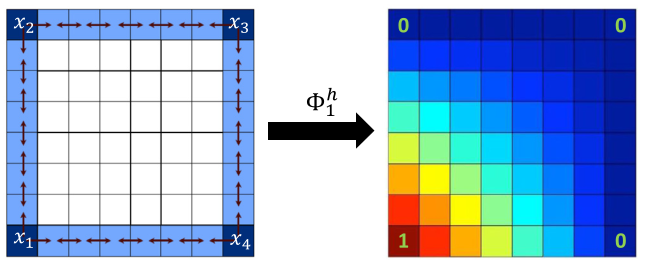
\includegraphics[scale=0.25]{./imgs/op_example.png}
        
        {\small Fonte: \cite{Hajibeygi_2020}}
    \end{textblock*}

    
    
    

    

    
\end{frame}

% \begin{frame}{Método Multiescala}
%     \begin{figure}[!ht]
%         \caption{Valores das funções de base para o vértice $x_{1}$}
%         \centering
%         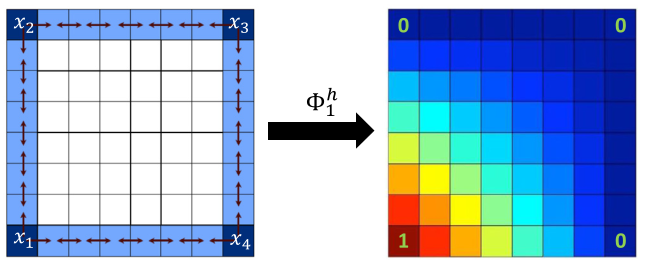
\includegraphics[scale=0.4]{./imgs/op_example.png}    
%         \label{fig:operador_method.1}

%         {\footnotesize Fonte: \cite{Hajibeygi_2020}}
%     \end{figure}
% \end{frame}

\begin{frame}{Método Multiescala}
    \justify
    % O operador de restrição utilizado nesse trabalho, que é responsável por realizar o \textit{Upscaling} das informações, é o operador clássico de volumes finitos, dado por \cite{Tene_2016}:
    Operador de Restrição:

    \begin{equation}
        \label{eq:multiescala.11}
        \restOperator = 
        \begin{cases}
            1 & \text{ se } \volf \in \volcoarse\\
            0 & \text{ caso contrário }
        \end{cases}.
    \end{equation}

    \begin{tikzpicture}[scale = 0.5]
    \def \Dx {12}
    \def \stp {1}
    \def \stpp {3}
  
    % style of grid
    \draw[fill=lightgray!80] (0,0) rectangle (\stp,\stp);
    \tikzset{gridstyle1/.style={color=lightgray,thin}}
    \draw[style=gridstyle1,step=\stp] (0,0) grid (\stpp,\stpp);
    \draw (\stp/2,\stp/2) node{$\volf$};
  
    % \draw plot coordinates{(\stp*2+\stp/2,\stp*2+\stp/2)} node[sloped] {$\Omega_{i}$};
    % \draw[line width=2pt,color=blue] (\Dx/2, 0) -- (0,0) -- (0,\Dx) -- (\Dx/2,\Dx);
    % \draw[line width=2pt,color=red] (\Dx/2, 0) -- (\Dx,0) -- (\Dx,\Dx) -- (\Dx/2,\Dx);
    % \draw[->, ultra thick] (-2,\Dx/2+1) node[sloped, left]{$\Gamma_{D}$} -- (0,\Dx/2);
    % \draw[->, ultra thick] (\Dx+2,\Dx/2+1) node[sloped, right]{$\Gamma_{N}$} -- (\Dx,\Dx/2);
    % \draw[fill=yellow!50] (0.5,0.5) circle (0.2);
    % \draw plot [mark=*, mark size=2] coordinates{(0.5,0.5)};
    % \draw[fill=yellow!50] (\Dx-0.5,\Dx-0.5) circle (0.2);
    % \draw plot [mark=*, mark size=2] coordinates{(\Dx-0.5,\Dx-0.5)};
    % \draw[->, ultra thick] (-1,1) node[sloped, left]{$\Gamma_{I}$} -- (0.5,0.5);
    % \draw[->, ultra thick] (\Dx+0.5,\Dx+0.5) node[sloped, right]{$\Gamma_{P}$} -- (\Dx-0.5,\Dx-0.5);
  
  \end{tikzpicture}
  
    
    \begin{textblock*}{5cm}(3cm,6.3cm) % {block width} (coords)
        \begin{tikzpicture}[scale = 0.5]
    \def \Dx {12}
    \def \stp {1}
    \def \stpp {3}
  
    % style of grid
    \tikzset{gridstyle1/.style={color=lightgray,thin}}
    \tikzset{gridstyle2/.style={color=black,line width=1pt}}
    % \draw[fill=red!30,draw=white] (\stp*2,\stp*2) rectangle (\stp*3,\stp*3);
    \draw[style=gridstyle1,step=\stp] (0,0) grid (\stpp,\stpp);
    \draw[fill=lightgray!80] (0,0) rectangle (\stpp,\stpp);
    \draw[style=gridstyle2,step=\stpp] (0,0) grid (\stpp,\stpp);
  
    \draw (\stpp/2,\stpp/2) node{$\volcoarse$};
    % \draw plot coordinates{(\stp*2+\stp/2,\stp*2+\stp/2)} node[sloped] {$\Omega_{i}$};
    % \draw[line width=2pt,color=blue] (\Dx/2, 0) -- (0,0) -- (0,\Dx) -- (\Dx/2,\Dx);
    % \draw[line width=2pt,color=red] (\Dx/2, 0) -- (\Dx,0) -- (\Dx,\Dx) -- (\Dx/2,\Dx);
    % \draw[->, ultra thick] (-2,\Dx/2+1) node[sloped, left]{$\Gamma_{D}$} -- (0,\Dx/2);
    % \draw[->, ultra thick] (\Dx+2,\Dx/2+1) node[sloped, right]{$\Gamma_{N}$} -- (\Dx,\Dx/2);
    % \draw[fill=yellow!50] (0.5,0.5) circle (0.2);
    % \draw plot [mark=*, mark size=2] coordinates{(0.5,0.5)};
    % \draw[fill=yellow!50] (\Dx-0.5,\Dx-0.5) circle (0.2);
    % \draw plot [mark=*, mark size=2] coordinates{(\Dx-0.5,\Dx-0.5)};
    % \draw[->, ultra thick] (-1,1) node[sloped, left]{$\Gamma_{I}$} -- (0.5,0.5);
    % \draw[->, ultra thick] (\Dx+0.5,\Dx+0.5) node[sloped, right]{$\Gamma_{P}$} -- (\Dx-0.5,\Dx-0.5);
    % \draw (\Dx/2,\Dx/2) node[sloped, above]{$\Omega$};
  \end{tikzpicture}
  
    \end{textblock*}

\end{frame}

\begin{frame}{Método Multiescala}
    \small
    \begin{gather*}
        \vectorPressure \approx \vectorMsPressure = \prolOperator \vectorCoarsePressure \\
        \fineTransmissibility \vectorPressure = \vectorfineSource  \longrightarrow \fineTransmissibility \prolOperator \vectorCoarsePressure = \vectorfineSource \\
        \restOperator \spaceum \fineTransmissibility \vectorPressure = \restOperator \vectorfineSource  \longrightarrow \coarseTransmissibility \vectorCoarsePressure = \coarseSourceTerm \\
        \coarseTransmissibility = \restOperator \spaceum \fineTransmissibility \prolOperator \\
        \coarseSourceTerm = \restOperator \vectorfineSource
    \end{gather*}

    \begin{description}[]
        \item $\vectorMsPressure$ = pressão multiescala;
        \item $\vectorCoarsePressure$ = pressão da escala grossa;
        \item $\coarseTransmissibility$ = matriz transmissibilidade da escala grossa;
        \item $\coarseSourceTerm$ = termo fonte da escala grossa;
        \item $\coarseTransmissibility \vectorCoarsePressure = \coarseSourceTerm$ : sistema linear da escala grossa
    \end{description}
\end{frame}

% \begin{frame}{Método Multiescala}
    
%     \small
    
%     \begin{itemize}
%         \justifying
%         \item Devido a imposição de desacoplamento para construção do operador de prolongamento, a pressão multiescala não garante conservação da massa em todos os volumes da malha fina, fazendo-se necessária a reconstrução da velocidade \cite{Moyner_2014,Jenny2003}.
%         \item Para esse fim, calcula-se o fluxo localmente, em cada volume da malha grossa primal, utilizando o fluxo do campo de pressão multiescala como condição de contorno.
%     \end{itemize}
    

    

%     % \begin{equation}
%     %     \label{eq:5_5_4.1}
%     %     \begin{cases}
%     %       (K \lambda_{T} \grad{\mathbf{P}''}) \cdot \vec{n} = (K \lambda_{T} \grad{\vectorMsPressure}) \text{ em } \partial \Omega_{I}\\
%     %       \div{K \lambda_{T} \grad{\mathbf{P}''}} = q \text{ em } \Omega_{I}\\
%     %     \end{cases}
%     %   \end{equation}

%     %   \begin{columns}
%     %     \begin{column}{0.5\textwidth}
%     %         \begin{description}[]
%     %             \item $\lambda_{T}$: mobilidade total do fluido = $\sum_{\phase} \lambda_{\phase}$ ;
%     %             \item $\lambda$: mobilidade do fluido = $\nicefrac{k_{r}}{\mu}$;
%     %             \item $k_r$: permeabilidade relativa 
%     %           \end{description}
%     %     \end{column}
%     %     \begin{column}{0.5\textwidth}
%     %         \begin{description}[]
%     %             \item $\partial \Omega_{I}$: Contorno do volume $\Omega_{I}$ 
%     %           \end{description}
%     %     \end{column}

%     %   \end{columns}
% \end{frame}

\begin{frame}{Método Multiescala}
    \begin{itemize}
        \item Recuperação do fluxo.
    \end{itemize}
    
\end{frame}

% \begin{frame}{Método Multiescala}
    
% \end{frame}


\begin{frame}{Método ADM}
    \small
    % A transferência de escala para o nível superior ($l$) é feita utilizando os operadores ADM da seguinte forma \cite{Cusini2016}:
    Operadores ADM \cite{Cusini2016}:

    \begin{equation}
        \label{eq:multinivel.1}
    (\prolOperatorAdm)^{1}_{0} (i,j) =
        \begin{cases}
            (\prolOperator)^{1}_{0} (i,j) \text{ se o volume pertence ao próximo nível}\\
            \delta_{ij} \text{ caso contrário},\\
        \end{cases}
    \end{equation}

    \begin{equation}
        \label{eq:multinivel.2}
    (\restOperatorAdm)^{0}_{1} (i,j) =
        \begin{cases}
            (\restOperator)^{0}_{1} (i,j) \text{ se o volume pertence ao próximo nível}\\
            \delta_{ij} \text{ caso contrário}.\\
        \end{cases}
    \end{equation}

\end{frame}

% \begin{frame}{Método ADM}
%     \begin{figure}
%         \caption{Representação dos conjuntos $\Omega^{l}$, $\Pi^{l}$ e $\Gamma^{l}$}
%         \begin{subfigure}{.3\textwidth}
%             \centering
%             \resizebox*{3cm}{!}{
%             \begin{tikzpicture}[scale = 0.25]
    \def \Dx {12}
    \def \stp {1}
    \def \stpp {3}
  
      \def \za {0}
      % \def \zb {8}
      \def \zb {10}
      % \def \zc {16}
      \def \zc {20}
      \def \compx {18}
      \def \rx {3}
      \def \rxx {9}
      \def \nx {\compx/\rx}
      \def \nxx {\compx/\rxx}
  
    % style of grid
      \tikzset{nivelstyle1/.style={fill=green,opacity=1,very thin,line join=round}}
      \tikzset{nivelstyle2/.style={fill=red,opacity=1,very thin,line join=round}}
      \tikzset{nivelstyle0/.style={fill=lightgray,opacity=1,very thin,line join=round}}
  
      \draw[style=nivelstyle2] (0,0) rectangle (\compx,\compx);
      \draw[step=\rxx] (0,0) grid (\compx,\compx);
      \draw[style=nivelstyle1] (0,\compx/2) rectangle (\compx/2,\compx);
      \draw[step=\rx] (0,\compx/2) grid (\compx/2,\compx);
      \draw[style=nivelstyle1] (\compx/2,0) rectangle (\compx,\compx/2);
      \draw[step=\rx] (\compx/2,0) grid (\compx,\compx/2);
      \draw[style=nivelstyle0] (0,\compx) rectangle (\rx,\compx-\rx);
      \draw[step=1] (0,\compx) grid (\rx,\compx-\rx);
      \draw[style=nivelstyle0] (\compx-\rx,0) rectangle (\compx,\rx);
      \draw[step=1] (\compx-\rx,0) grid (\compx,\rx);
  
    % \draw[fill=red!80,draw=white] (\stp, \stp) rectangle (2*\stp, 2*\stp);
    % \draw[fill=red!80,draw=white] (4*\stp, \stp) rectangle (5*\stp, 2*\stp);
    % \draw[fill=red!80,draw=white] (7*\stp, \stp) rectangle (8*\stp, 2*\stp);
    % \draw[fill=red!80,draw=white] (10*\stp, \stp) rectangle (11*\stp, 2*\stp);
      %
    % \draw[fill=red!80,draw=white] (\stp, 4*\stp) rectangle (2*\stp, 5*\stp);
    % % \draw[fill=red!80,draw=white] (4*\stp, 4*\stp) rectangle (5*\stp, 5*\stp);
    % % \draw[fill=red!80,draw=white] (7*\stp, 4*\stp) rectangle (8*\stp, 5*\stp);
    % \draw[fill=red!80,draw=white] (10*\stp, 4*\stp) rectangle (11*\stp, 5*\stp);
      %
    % \draw[fill=red!80,draw=white] (\stp, 7*\stp) rectangle (2*\stp, 8*\stp);
    % \draw[fill=red!80,draw=white] (4*\stp, 7*\stp) rectangle (5*\stp, 8*\stp);
    % \draw[fill=red!80,draw=white] (7*\stp, 7*\stp) rectangle (8*\stp, 8*\stp);
    % \draw[fill=red!80,draw=white] (10*\stp, 7*\stp) rectangle (11*\stp, 8*\stp);
      %
    % \draw[fill=red!80,draw=white] (\stp, 10*\stp) rectangle (2*\stp, 11*\stp);
    % \draw[fill=red!80,draw=white] (4*\stp, 10*\stp) rectangle (5*\stp, 11*\stp);
    % \draw[fill=red!80,draw=white] (7*\stp, 10*\stp) rectangle (8*\stp, 11*\stp);
    % \draw[fill=red!80,draw=white] (10*\stp, 10*\stp) rectangle (11*\stp, 11*\stp);
      %
    % % \draw[fill=red!30,draw=white] (\stp*2,\stp*2) rectangle (\stp*3,\stp*3);
    % \draw[style=gridstyle1,step=\stp] (0,0) grid (\Dx,\Dx);
    % \draw[style=gridstyle2,step=\stpp] (0,0) grid (\Dx,\Dx);
      %
    % \draw[fill=lightgray!80,draw=black,opacity=0.6] (\stpp+\stp, \stpp+\stp) rectangle (2*\stpp+2*\stp, 2*\stpp+2*\stp);
    % \draw[fill=red!80,draw=none] (4*\stp, 4*\stp) rectangle (5*\stp, 5*\stp);
    % \draw[fill=red!80,draw=none] (7*\stp, 4*\stp) rectangle (8*\stp, 5*\stp);
    % \draw[fill=red!80,draw=none] (4*\stp, 7*\stp) rectangle (5*\stp, 8*\stp);
    % \draw[fill=red!80,draw=none] (7*\stp, 7*\stp) rectangle (8*\stp, 8*\stp);
    % \draw (2*\stpp+\stp/2,2*\stpp+\stp/2) node{$\voldual$};
  
    % \draw plot coordinates{(\stp*2+\stp/2,\stp*2+\stp/2)} node[sloped] {$\Omega_{i}$};
    % \draw[line width=2pt,color=blue] (\Dx/2, 0) -- (0,0) -- (0,\Dx) -- (\Dx/2,\Dx);
    % \draw[line width=2pt,color=red] (\Dx/2, 0) -- (\Dx,0) -- (\Dx,\Dx) -- (\Dx/2,\Dx);
    % \draw[->, ultra thick] (-2,\Dx/2+1) node[sloped, left]{$\Gamma_{D}$} -- (0,\Dx/2);
    % \draw[->, ultra thick] (\Dx+2,\Dx/2+1) node[sloped, right]{$\Gamma_{N}$} -- (\Dx,\Dx/2);
    % \draw[fill=yellow!50] (0.5,0.5) circle (0.2);
    % \draw plot [mark=*, mark size=2] coordinates{(0.5,0.5)};
    % \draw[fill=yellow!50] (\Dx-0.5,\Dx-0.5) circle (0.2);
    % \draw plot [mark=*, mark size=2] coordinates{(\Dx-0.5,\Dx-0.5)};
    % \draw[->, ultra thick] (-1,1) node[sloped, left]{$\Gamma_{I}$} -- (0.5,0.5);
    % \draw[->, ultra thick] (\Dx+0.5,\Dx+0.5) node[sloped, right]{$\Gamma_{P}$} -- (\Dx-0.5,\Dx-0.5);
    % \draw (\Dx/2,\Dx/2) node[sloped, above]{$\Omega$};
  \end{tikzpicture}
  }
%             \subcaption{$\Omega^{l}$}
%             \label{fig:multinivel.2.a}
%         \end{subfigure}
%         \begin{subfigure}{.3\textwidth}
%             \centering
%             \resizebox*{3cm}{!}{
%             \begin{tikzpicture}[scale = 0.25]
    \def \Dx {12}
    \def \stp {1}
    \def \stpp {3}
  
      \def \za {0}
      % \def \zb {8}
      \def \zb {10}
      % \def \zc {16}
      \def \zc {20}
      \def \compx {18}
      \def \rx {3}
      \def \rxx {9}
      \def \nx {\compx/\rx}
      \def \nxx {\compx/\rxx}
  
    % style of grid
      \tikzset{nivelstyle1/.style={fill=green,opacity=1,very thin,line join=round}}
      \tikzset{nivelstyle2/.style={fill=red,opacity=1,very thin,line join=round}}
      \tikzset{nivelstyle0/.style={fill=lightgray,opacity=1,very thin,line join=round}}
  
      % \draw[style=nivelstyle2] (0,0) rectangle (\compx,\compx);
      \draw[style=nivelstyle2] (0,0) rectangle (\compx,\compx);
    \draw[step=\rxx] (0,0) grid (\compx,\compx);
    % \draw[style=nivelstyle2] (\compx/2,\compx/2) rectangle (\compx,\compx);
      % \draw[style=nivelstyle1] (0,\compx/2) rectangle (\compx/2,\compx);
      % \draw[step=\rx] (0,\compx/2) grid (\compx/2,\compx);
      % \draw[style=nivelstyle1] (\compx/2,0) rectangle (\compx,\compx/2);
      % \draw[step=\rx] (\compx/2,0) grid (\compx,\compx/2);
      % \draw[fill=white] (0,\compx) rectangle (\rx,\compx-\rx);
      % \draw[step=1] (0,\compx) grid (\rx,\compx-\rx);
      % \draw[style=nivelstyle0] (\compx-\rx,0) rectangle (\compx,\rx);
      % \draw[fill=white] (\compx-\rx,0) rectangle (\compx,\rx);
  
    % \draw[fill=red!80,draw=white] (\stp, \stp) rectangle (2*\stp, 2*\stp);
    % \draw[fill=red!80,draw=white] (4*\stp, \stp) rectangle (5*\stp, 2*\stp);
    % \draw[fill=red!80,draw=white] (7*\stp, \stp) rectangle (8*\stp, 2*\stp);
    % \draw[fill=red!80,draw=white] (10*\stp, \stp) rectangle (11*\stp, 2*\stp);
      %
    % \draw[fill=red!80,draw=white] (\stp, 4*\stp) rectangle (2*\stp, 5*\stp);
    % % \draw[fill=red!80,draw=white] (4*\stp, 4*\stp) rectangle (5*\stp, 5*\stp);
    % % \draw[fill=red!80,draw=white] (7*\stp, 4*\stp) rectangle (8*\stp, 5*\stp);
    % \draw[fill=red!80,draw=white] (10*\stp, 4*\stp) rectangle (11*\stp, 5*\stp);
      %
    % \draw[fill=red!80,draw=white] (\stp, 7*\stp) rectangle (2*\stp, 8*\stp);
    % \draw[fill=red!80,draw=white] (4*\stp, 7*\stp) rectangle (5*\stp, 8*\stp);
    % \draw[fill=red!80,draw=white] (7*\stp, 7*\stp) rectangle (8*\stp, 8*\stp);
    % \draw[fill=red!80,draw=white] (10*\stp, 7*\stp) rectangle (11*\stp, 8*\stp);
      %
    % \draw[fill=red!80,draw=white] (\stp, 10*\stp) rectangle (2*\stp, 11*\stp);
    % \draw[fill=red!80,draw=white] (4*\stp, 10*\stp) rectangle (5*\stp, 11*\stp);
    % \draw[fill=red!80,draw=white] (7*\stp, 10*\stp) rectangle (8*\stp, 11*\stp);
    % \draw[fill=red!80,draw=white] (10*\stp, 10*\stp) rectangle (11*\stp, 11*\stp);
      %
    % % \draw[fill=red!30,draw=white] (\stp*2,\stp*2) rectangle (\stp*3,\stp*3);
    % \draw[style=gridstyle1,step=\stp] (0,0) grid (\Dx,\Dx);
    % \draw[style=gridstyle2,step=\stpp] (0,0) grid (\Dx,\Dx);
      %
    % \draw[fill=lightgray!80,draw=black,opacity=0.6] (\stpp+\stp, \stpp+\stp) rectangle (2*\stpp+2*\stp, 2*\stpp+2*\stp);
    % \draw[fill=red!80,draw=none] (4*\stp, 4*\stp) rectangle (5*\stp, 5*\stp);
    % \draw[fill=red!80,draw=none] (7*\stp, 4*\stp) rectangle (8*\stp, 5*\stp);
    % \draw[fill=red!80,draw=none] (4*\stp, 7*\stp) rectangle (5*\stp, 8*\stp);
    % \draw[fill=red!80,draw=none] (7*\stp, 7*\stp) rectangle (8*\stp, 8*\stp);
    % \draw (2*\stpp+\stp/2,2*\stpp+\stp/2) node{$\voldual$};
  
    % \draw plot coordinates{(\stp*2+\stp/2,\stp*2+\stp/2)} node[sloped] {$\Omega_{i}$};
    % \draw[line width=2pt,color=blue] (\Dx/2, 0) -- (0,0) -- (0,\Dx) -- (\Dx/2,\Dx);
    % \draw[line width=2pt,color=red] (\Dx/2, 0) -- (\Dx,0) -- (\Dx,\Dx) -- (\Dx/2,\Dx);
    % \draw[->, ultra thick] (-2,\Dx/2+1) node[sloped, left]{$\Gamma_{D}$} -- (0,\Dx/2);
    % \draw[->, ultra thick] (\Dx+2,\Dx/2+1) node[sloped, right]{$\Gamma_{N}$} -- (\Dx,\Dx/2);
    % \draw[fill=yellow!50] (0.5,0.5) circle (0.2);
    % \draw plot [mark=*, mark size=2] coordinates{(0.5,0.5)};
    % \draw[fill=yellow!50] (\Dx-0.5,\Dx-0.5) circle (0.2);
    % \draw plot [mark=*, mark size=2] coordinates{(\Dx-0.5,\Dx-0.5)};
    % \draw[->, ultra thick] (-1,1) node[sloped, left]{$\Gamma_{I}$} -- (0.5,0.5);
    % \draw[->, ultra thick] (\Dx+0.5,\Dx+0.5) node[sloped, right]{$\Gamma_{P}$} -- (\Dx-0.5,\Dx-0.5);
    % \draw (\Dx/2,\Dx/2) node[sloped, above]{$\Omega$};
  \end{tikzpicture}
  }
%             \subcaption{$\Pi^{l}$}
%             \label{fig:multinivel.2.b}
%         \end{subfigure}
%         \begin{subfigure}{.3\textwidth}
%             \centering
%             \resizebox*{3cm}{!}{
%             \begin{tikzpicture}[scale = 0.25]
    \def \Dx {12}
    \def \stp {1}
    \def \stpp {3}
  
      \def \za {0}
      % \def \zb {8}
      \def \zb {10}
      % \def \zc {16}
      \def \zc {20}
      \def \compx {18}
      \def \rx {3}
      \def \rxx {9}
      \def \nx {\compx/\rx}
      \def \nxx {\compx/\rxx}
  
    % style of grid
      \tikzset{nivelstyle1/.style={fill=green,opacity=1,very thin,line join=round}}
      \tikzset{nivelstyle2/.style={fill=red,opacity=1,very thin,line join=round}}
      \tikzset{nivelstyle0/.style={fill=lightgray,opacity=1,very thin,line join=round}}
  
      % \draw[style=nivelstyle2] (0,0) rectangle (\compx,\compx);
      \draw (0,0) rectangle (\compx,\compx);
    \draw[style=nivelstyle2] (0,0) rectangle (\compx/2,\compx/2);
    \draw[style=nivelstyle2] (\compx/2,\compx/2) rectangle (\compx,\compx);
      % \draw[style=nivelstyle1] (0,\compx/2) rectangle (\compx/2,\compx);
      % \draw[step=\rx] (0,\compx/2) grid (\compx/2,\compx);
      % \draw[style=nivelstyle1] (\compx/2,0) rectangle (\compx,\compx/2);
      % \draw[step=\rx] (\compx/2,0) grid (\compx,\compx/2);
      % \draw[fill=white] (0,\compx) rectangle (\rx,\compx-\rx);
      % \draw[step=1] (0,\compx) grid (\rx,\compx-\rx);
      % \draw[style=nivelstyle0] (\compx-\rx,0) rectangle (\compx,\rx);
      % \draw[fill=white] (\compx-\rx,0) rectangle (\compx,\rx);
  
    % \draw[fill=red!80,draw=white] (\stp, \stp) rectangle (2*\stp, 2*\stp);
    % \draw[fill=red!80,draw=white] (4*\stp, \stp) rectangle (5*\stp, 2*\stp);
    % \draw[fill=red!80,draw=white] (7*\stp, \stp) rectangle (8*\stp, 2*\stp);
    % \draw[fill=red!80,draw=white] (10*\stp, \stp) rectangle (11*\stp, 2*\stp);
      %
    % \draw[fill=red!80,draw=white] (\stp, 4*\stp) rectangle (2*\stp, 5*\stp);
    % % \draw[fill=red!80,draw=white] (4*\stp, 4*\stp) rectangle (5*\stp, 5*\stp);
    % % \draw[fill=red!80,draw=white] (7*\stp, 4*\stp) rectangle (8*\stp, 5*\stp);
    % \draw[fill=red!80,draw=white] (10*\stp, 4*\stp) rectangle (11*\stp, 5*\stp);
      %
    % \draw[fill=red!80,draw=white] (\stp, 7*\stp) rectangle (2*\stp, 8*\stp);
    % \draw[fill=red!80,draw=white] (4*\stp, 7*\stp) rectangle (5*\stp, 8*\stp);
    % \draw[fill=red!80,draw=white] (7*\stp, 7*\stp) rectangle (8*\stp, 8*\stp);
    % \draw[fill=red!80,draw=white] (10*\stp, 7*\stp) rectangle (11*\stp, 8*\stp);
      %
    % \draw[fill=red!80,draw=white] (\stp, 10*\stp) rectangle (2*\stp, 11*\stp);
    % \draw[fill=red!80,draw=white] (4*\stp, 10*\stp) rectangle (5*\stp, 11*\stp);
    % \draw[fill=red!80,draw=white] (7*\stp, 10*\stp) rectangle (8*\stp, 11*\stp);
    % \draw[fill=red!80,draw=white] (10*\stp, 10*\stp) rectangle (11*\stp, 11*\stp);
      %
    % % \draw[fill=red!30,draw=white] (\stp*2,\stp*2) rectangle (\stp*3,\stp*3);
    % \draw[style=gridstyle1,step=\stp] (0,0) grid (\Dx,\Dx);
    % \draw[style=gridstyle2,step=\stpp] (0,0) grid (\Dx,\Dx);
      %
    % \draw[fill=lightgray!80,draw=black,opacity=0.6] (\stpp+\stp, \stpp+\stp) rectangle (2*\stpp+2*\stp, 2*\stpp+2*\stp);
    % \draw[fill=red!80,draw=none] (4*\stp, 4*\stp) rectangle (5*\stp, 5*\stp);
    % \draw[fill=red!80,draw=none] (7*\stp, 4*\stp) rectangle (8*\stp, 5*\stp);
    % \draw[fill=red!80,draw=none] (4*\stp, 7*\stp) rectangle (5*\stp, 8*\stp);
    % \draw[fill=red!80,draw=none] (7*\stp, 7*\stp) rectangle (8*\stp, 8*\stp);
    % \draw (2*\stpp+\stp/2,2*\stpp+\stp/2) node{$\voldual$};
  
    % \draw plot coordinates{(\stp*2+\stp/2,\stp*2+\stp/2)} node[sloped] {$\Omega_{i}$};
    % \draw[line width=2pt,color=blue] (\Dx/2, 0) -- (0,0) -- (0,\Dx) -- (\Dx/2,\Dx);
    % \draw[line width=2pt,color=red] (\Dx/2, 0) -- (\Dx,0) -- (\Dx,\Dx) -- (\Dx/2,\Dx);
    % \draw[->, ultra thick] (-2,\Dx/2+1) node[sloped, left]{$\Gamma_{D}$} -- (0,\Dx/2);
    % \draw[->, ultra thick] (\Dx+2,\Dx/2+1) node[sloped, right]{$\Gamma_{N}$} -- (\Dx,\Dx/2);
    % \draw[fill=yellow!50] (0.5,0.5) circle (0.2);
    % \draw plot [mark=*, mark size=2] coordinates{(0.5,0.5)};
    % \draw[fill=yellow!50] (\Dx-0.5,\Dx-0.5) circle (0.2);
    % \draw plot [mark=*, mark size=2] coordinates{(\Dx-0.5,\Dx-0.5)};
    % \draw[->, ultra thick] (-1,1) node[sloped, left]{$\Gamma_{I}$} -- (0.5,0.5);
    % \draw[->, ultra thick] (\Dx+0.5,\Dx+0.5) node[sloped, right]{$\Gamma_{P}$} -- (\Dx-0.5,\Dx-0.5);
    % \draw (\Dx/2,\Dx/2) node[sloped, above]{$\Omega$};
  \end{tikzpicture}
  }
%             \subcaption{$\Gamma^{l}$}
%             \label{fig:multinivel.2.c}
%         \end{subfigure}
%         \label{fig:multinivel.2}
%     \end{figure}

%     \begin{equation}
%         \label{eq:multinivel.3}
%         ( \restOperatorAdm )^{l-1}_{l} ... ( \restOperatorAdm )^{0}_{1} \fineTransmissibility (\prolOperatorAdm)^{l}_{l-1} ... (\prolOperatorAdm)^{1}_{0} \vectorPressureAdm = ( \restOperatorAdm )^{l-1}_{l} ... ( \restOperatorAdm )^{0}_{1} \vectorfineSource,
%     \end{equation}
% \end{frame}

% \begin{frame}{Método NU-ADM}
%     A fim de diminuir a quantidade de volumes na malha ADM, foi desenvolvido por \citeonline{Araujo_dos_Santos_2022} o método ADM não uniforme (NU-ADM), permitindo que os volumes não engrossados não estejam necessariamente agrupados de acordo com o volume da malha grossa, reduzindo o sistema linear da escala ADM.


% \end{frame}

\begin{frame}{Método NU-ADM}
    \begin{figure}
        % \caption{Diferença entre os métodos ADM e NU-ADM}
        \begin{subfigure}{.48\textwidth}
            \centering
            \resizebox*{5cm}{!}{
            \begin{tikzpicture}[scale = 0.25]
    \def \Dx {12}
    \def \stp {1}
    \def \stpp {3}
  
      \def \za {0}
      % \def \zb {8}
      \def \zb {10}
      % \def \zc {16}
      \def \zc {20}
      \def \compx {18}
      \def \rx {3}
      \def \rxx {9}
      \def \nx {\compx/\rx}
      \def \nxx {\compx/\rxx}
  
    % style of grid
      \tikzset{nivelstyle1/.style={fill=green,opacity=1,very thin,line join=round}}
      \tikzset{nivelstyle2/.style={fill=red,opacity=1,very thin,line join=round}}
      \tikzset{nivelstyle0/.style={fill=lightgray,opacity=1,very thin,line join=round}}
  
      % \draw[style=nivelstyle2] (0,0) rectangle (\compx,\compx);
      % \draw[step=\rxx] (0,0) grid (\compx,\compx);
      % \draw[style=nivelstyle1] (0,\compx/2) rectangle (\compx/2,\compx);
      % \draw[step=\rx] (0,\compx/2) grid (\compx/2,\compx);
      \fill[style=nivelstyle1] (0,0) rectangle (\compx,\compx);
      \draw[step=\rx] (0,0) grid (\compx,\compx);
      % \draw[style=nivelstyle1] (\compx/2,0) rectangle (\compx,\compx/2);
      % \draw[step=\rx] (\compx/2,0) grid (\compx,\compx/2);
      \fill[style=nivelstyle0] (0,\compx) rectangle (\rx,\compx-\rx);
      \draw[step=1] (0,\compx) grid (\rx,\compx-\rx);
      \fill[style=nivelstyle0] (\compx-\rx,0) rectangle (\compx,\rx);
      \draw[step=1] (\compx-\rx,0) grid (\compx,\rx);
  
    % \draw[fill=red!80,draw=white] (\stp, \stp) rectangle (2*\stp, 2*\stp);
    % \draw[fill=red!80,draw=white] (4*\stp, \stp) rectangle (5*\stp, 2*\stp);
    % \draw[fill=red!80,draw=white] (7*\stp, \stp) rectangle (8*\stp, 2*\stp);
    % \draw[fill=red!80,draw=white] (10*\stp, \stp) rectangle (11*\stp, 2*\stp);
      %
    % \draw[fill=red!80,draw=white] (\stp, 4*\stp) rectangle (2*\stp, 5*\stp);
    % % \draw[fill=red!80,draw=white] (4*\stp, 4*\stp) rectangle (5*\stp, 5*\stp);
    % % \draw[fill=red!80,draw=white] (7*\stp, 4*\stp) rectangle (8*\stp, 5*\stp);
    % \draw[fill=red!80,draw=white] (10*\stp, 4*\stp) rectangle (11*\stp, 5*\stp);
      %
    % \draw[fill=red!80,draw=white] (\stp, 7*\stp) rectangle (2*\stp, 8*\stp);
    % \draw[fill=red!80,draw=white] (4*\stp, 7*\stp) rectangle (5*\stp, 8*\stp);
    % \draw[fill=red!80,draw=white] (7*\stp, 7*\stp) rectangle (8*\stp, 8*\stp);
    % \draw[fill=red!80,draw=white] (10*\stp, 7*\stp) rectangle (11*\stp, 8*\stp);
      %
    % \draw[fill=red!80,draw=white] (\stp, 10*\stp) rectangle (2*\stp, 11*\stp);
    % \draw[fill=red!80,draw=white] (4*\stp, 10*\stp) rectangle (5*\stp, 11*\stp);
    % \draw[fill=red!80,draw=white] (7*\stp, 10*\stp) rectangle (8*\stp, 11*\stp);
    % \draw[fill=red!80,draw=white] (10*\stp, 10*\stp) rectangle (11*\stp, 11*\stp);
      %
    % % \draw[fill=red!30,draw=white] (\stp*2,\stp*2) rectangle (\stp*3,\stp*3);
    % \draw[style=gridstyle1,step=\stp] (0,0) grid (\Dx,\Dx);
    % \draw[style=gridstyle2,step=\stpp] (0,0) grid (\Dx,\Dx);
      %
    % \draw[fill=lightgray!80,draw=black,opacity=0.6] (\stpp+\stp, \stpp+\stp) rectangle (2*\stpp+2*\stp, 2*\stpp+2*\stp);
    % \draw[fill=red!80,draw=none] (4*\stp, 4*\stp) rectangle (5*\stp, 5*\stp);
    % \draw[fill=red!80,draw=none] (7*\stp, 4*\stp) rectangle (8*\stp, 5*\stp);
    % \draw[fill=red!80,draw=none] (4*\stp, 7*\stp) rectangle (5*\stp, 8*\stp);
    % \draw[fill=red!80,draw=none] (7*\stp, 7*\stp) rectangle (8*\stp, 8*\stp);
    % \draw (2*\stpp+\stp/2,2*\stpp+\stp/2) node{$\voldual$};
  
    % \draw plot coordinates{(\stp*2+\stp/2,\stp*2+\stp/2)} node[sloped] {$\Omega_{i}$};
    % \draw[line width=2pt,color=blue] (\Dx/2, 0) -- (0,0) -- (0,\Dx) -- (\Dx/2,\Dx);
    % \draw[line width=2pt,color=red] (\Dx/2, 0) -- (\Dx,0) -- (\Dx,\Dx) -- (\Dx/2,\Dx);
    % \draw[->, ultra thick] (-2,\Dx/2+1) node[sloped, left]{$\Gamma_{D}$} -- (0,\Dx/2);
    % \draw[->, ultra thick] (\Dx+2,\Dx/2+1) node[sloped, right]{$\Gamma_{N}$} -- (\Dx,\Dx/2);
    % \draw[fill=yellow!50] (0.5,0.5) circle (0.2);
    % \draw plot [mark=*, mark size=2] coordinates{(0.5,0.5)};
    % \draw[fill=yellow!50] (\Dx-0.5,\Dx-0.5) circle (0.2);
    % \draw plot [mark=*, mark size=2] coordinates{(\Dx-0.5,\Dx-0.5)};
    % \draw[->, ultra thick] (-1,1) node[sloped, left]{$\Gamma_{I}$} -- (0.5,0.5);
    % \draw[->, ultra thick] (\Dx+0.5,\Dx+0.5) node[sloped, right]{$\Gamma_{P}$} -- (\Dx-0.5,\Dx-0.5);
    % \draw (\Dx/2,\Dx/2) node[sloped, above]{$\Omega$};
  \end{tikzpicture}
  }
            \subcaption{Método ADM}
            \label{fig:multinivel.3.a}
        \end{subfigure}
        \begin{subfigure}{.48\textwidth}
            \centering
            \resizebox*{5cm}{!}{
            \begin{tikzpicture}[scale = 0.25]
  \def \Dx {12}
  \def \stp {1}
  \def \stpp {3}

    \def \za {0}
    % \def \zb {8}
    \def \zb {10}
    % \def \zc {16}
    \def \zc {20}
    \def \compx {18}
    \def \rx {3}
    \def \rxx {9}
    \def \nx {\compx/\rx}
    \def \nxx {\compx/\rxx}

  % style of grid
    \tikzset{nivelstyle1/.style={fill=green,opacity=1,very thin,line join=round}}
    \tikzset{nivelstyle2/.style={fill=red,opacity=1,very thin,line join=round}}
    \tikzset{nivelstyle0/.style={fill=lightgray,opacity=1,very thin,line join=round}}

    % \draw[style=nivelstyle2] (0,0) rectangle (\compx,\compx);
    % \draw[step=\rxx] (0,0) grid (\compx,\compx);
    % \draw[style=nivelstyle1] (0,\compx/2) rectangle (\compx/2,\compx);
    % \draw[step=\rx] (0,\compx/2) grid (\compx/2,\compx);
    \fill[style=nivelstyle1] (0,0) rectangle (\compx,\compx);
    \draw[step=\rx] (0,0) grid (\compx,\compx);
    % \draw[style=nivelstyle1] (\compx/2,0) rectangle (\compx,\compx/2);
    % \draw[step=\rx] (\compx/2,0) grid (\compx,\compx/2);
    \fill[style=nivelstyle0] (0,\compx) rectangle (2*\rx/3,\compx-2*\rx/3);
    \draw[step=1] (0,\compx) grid (2*\rx/3,\compx-2*\rx/3);
    \fill[style=nivelstyle0] (\compx-2*\rx/3,0) rectangle (\compx,2*\rx/3);
    \draw[step=1] (\compx-2*\rx/3,0) grid (\compx,2*\rx/3);

  % \draw[fill=red!80,draw=white] (\stp, \stp) rectangle (2*\stp, 2*\stp);
  % \draw[fill=red!80,draw=white] (4*\stp, \stp) rectangle (5*\stp, 2*\stp);
  % \draw[fill=red!80,draw=white] (7*\stp, \stp) rectangle (8*\stp, 2*\stp);
  % \draw[fill=red!80,draw=white] (10*\stp, \stp) rectangle (11*\stp, 2*\stp);
    %
  % \draw[fill=red!80,draw=white] (\stp, 4*\stp) rectangle (2*\stp, 5*\stp);
  % % \draw[fill=red!80,draw=white] (4*\stp, 4*\stp) rectangle (5*\stp, 5*\stp);
  % % \draw[fill=red!80,draw=white] (7*\stp, 4*\stp) rectangle (8*\stp, 5*\stp);
  % \draw[fill=red!80,draw=white] (10*\stp, 4*\stp) rectangle (11*\stp, 5*\stp);
    %
  % \draw[fill=red!80,draw=white] (\stp, 7*\stp) rectangle (2*\stp, 8*\stp);
  % \draw[fill=red!80,draw=white] (4*\stp, 7*\stp) rectangle (5*\stp, 8*\stp);
  % \draw[fill=red!80,draw=white] (7*\stp, 7*\stp) rectangle (8*\stp, 8*\stp);
  % \draw[fill=red!80,draw=white] (10*\stp, 7*\stp) rectangle (11*\stp, 8*\stp);
    %
  % \draw[fill=red!80,draw=white] (\stp, 10*\stp) rectangle (2*\stp, 11*\stp);
  % \draw[fill=red!80,draw=white] (4*\stp, 10*\stp) rectangle (5*\stp, 11*\stp);
  % \draw[fill=red!80,draw=white] (7*\stp, 10*\stp) rectangle (8*\stp, 11*\stp);
  % \draw[fill=red!80,draw=white] (10*\stp, 10*\stp) rectangle (11*\stp, 11*\stp);
    %
  % % \draw[fill=red!30,draw=white] (\stp*2,\stp*2) rectangle (\stp*3,\stp*3);
  % \draw[style=gridstyle1,step=\stp] (0,0) grid (\Dx,\Dx);
  % \draw[style=gridstyle2,step=\stpp] (0,0) grid (\Dx,\Dx);
    %
  % \draw[fill=lightgray!80,draw=black,opacity=0.6] (\stpp+\stp, \stpp+\stp) rectangle (2*\stpp+2*\stp, 2*\stpp+2*\stp);
  % \draw[fill=red!80,draw=none] (4*\stp, 4*\stp) rectangle (5*\stp, 5*\stp);
  % \draw[fill=red!80,draw=none] (7*\stp, 4*\stp) rectangle (8*\stp, 5*\stp);
  % \draw[fill=red!80,draw=none] (4*\stp, 7*\stp) rectangle (5*\stp, 8*\stp);
  % \draw[fill=red!80,draw=none] (7*\stp, 7*\stp) rectangle (8*\stp, 8*\stp);
  % \draw (2*\stpp+\stp/2,2*\stpp+\stp/2) node{$\voldual$};

  % \draw plot coordinates{(\stp*2+\stp/2,\stp*2+\stp/2)} node[sloped] {$\Omega_{i}$};
  % \draw[line width=2pt,color=blue] (\Dx/2, 0) -- (0,0) -- (0,\Dx) -- (\Dx/2,\Dx);
  % \draw[line width=2pt,color=red] (\Dx/2, 0) -- (\Dx,0) -- (\Dx,\Dx) -- (\Dx/2,\Dx);
  % \draw[->, ultra thick] (-2,\Dx/2+1) node[sloped, left]{$\Gamma_{D}$} -- (0,\Dx/2);
  % \draw[->, ultra thick] (\Dx+2,\Dx/2+1) node[sloped, right]{$\Gamma_{N}$} -- (\Dx,\Dx/2);
  % \draw[fill=yellow!50] (0.5,0.5) circle (0.2);
  % \draw plot [mark=*, mark size=2] coordinates{(0.5,0.5)};
  % \draw[fill=yellow!50] (\Dx-0.5,\Dx-0.5) circle (0.2);
  % \draw plot [mark=*, mark size=2] coordinates{(\Dx-0.5,\Dx-0.5)};
  % \draw[->, ultra thick] (-1,1) node[sloped, left]{$\Gamma_{I}$} -- (0.5,0.5);
  % \draw[->, ultra thick] (\Dx+0.5,\Dx+0.5) node[sloped, right]{$\Gamma_{P}$} -- (\Dx-0.5,\Dx-0.5);
  % \draw (\Dx/2,\Dx/2) node[sloped, above]{$\Omega$};
\end{tikzpicture}}
            \subcaption{Método NU-ADM}
            \label{fig:multinivel.3.b}
        \end{subfigure}
        \label{fig:multinivel.2}
    \end{figure}

\end{frame}

\section{Objetivos}

% \subsection{Geral}
\begin{frame}{Objetivos}

    \begin{block}<1->{Geral}
        \begin{itemize}
            \item Desenvolver uma bliblioteca na linguagem Python que realize a transferência de escala, aplicando o método ADM não uniforme (NU-ADM) em modelos que lidam com escoamento composicional.
        \end{itemize}
    \end{block}

    \begin{block}<2->{Específicos}
        \begin{itemize}
            \item Desenvolver um interpretador os dados do reservatório
            \item Aplicar o método NU-ADM no modelo composicional IMPEC
            \item Comparar a solução da malha fina com a obtida por meio do método NU-ADM
        \end{itemize}
    \end{block}
    
\end{frame}

\section{Metodologia}
\begin{frame}{Seleção dos níveis}
    \small
    \begin{itemize}
        \justifying
        \item Volumes com prescrições;
        \item $\Delta \Saturation_{lim}$;
        \item Número de mols negativo.
    \end{itemize}
\end{frame}

\begin{frame}{Operador de Prolongamento}
    \small
    \begin{itemize}
        \item  Método AMS (\textit{Algebraic Multiscale Solver}) \cite{Wang2015}
    \end{itemize}

    \begin{figure}[!ht]
        
        \begin{subfigure}{.3\textwidth}
            \centering
            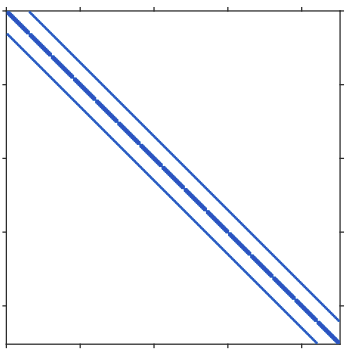
\includegraphics[scale=0.27]{./imgs/im10.png}
            \subcaption{$\fineTransmissibility$}
            \label{fig:multiescala.4.a}
        \end{subfigure}
        \begin{subfigure}{.3\textwidth}
            \centering
            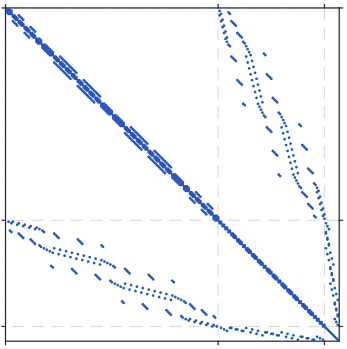
\includegraphics[scale=0.27]{./imgs/im11.png}
            \subcaption{\finewirebasketMatrix}
            \label{fig:multiescala.4.b}
        \end{subfigure}
        \begin{subfigure}{.3\textwidth}
            \centering
            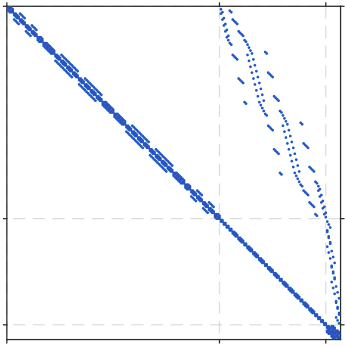
\includegraphics[scale=0.27]{./imgs/im12.png}
            \subcaption{$\finewirebasketMatrixMod$}
            \label{fig:multiescala.4.c}
        \end{subfigure}
        
        {\footnotesize Fonte:\cite{Magri2015}}
        \label{fig:multiescala.4}
    \end{figure}

    \newcommand{\deltaimg}{3.8cm}
    \newcommand{\deltaimgg}{3.65cm}
    \newcommand{\deltaimggg}{0.25cm}

    \begin{textblock*}{5cm}(5.7cm,4.1cm-\deltaimggg)
        F
    \end{textblock*}

    \begin{textblock*}{5cm}(7.2cm,4.1cm-\deltaimggg)
        A
    \end{textblock*}

    \begin{textblock*}{5cm}(7.8cm,4.1cm-\deltaimggg)
        V
    \end{textblock*}

    \begin{textblock*}{5cm}(4.5cm,5.4cm-\deltaimggg)
        F
    \end{textblock*}

    \begin{textblock*}{5cm}(4.5cm,6.9cm-\deltaimggg)
        A
    \end{textblock*}

    \begin{textblock*}{5cm}(4.5cm,7.45cm-\deltaimggg)
        V
    \end{textblock*}

    \begin{textblock*}{5cm}(5.7cm+\deltaimg,4.1cm-\deltaimggg)
        F
    \end{textblock*}

    \begin{textblock*}{5cm}(7.2cm+\deltaimg,4.1cm-\deltaimggg)
        A
    \end{textblock*}

    \begin{textblock*}{5cm}(7.8cm+3.65cm,4.1cm-\deltaimggg)
        V
    \end{textblock*}

    \begin{textblock*}{5cm}(4.5cm+\deltaimgg,5.4cm-\deltaimggg)
        F
    \end{textblock*}

    \begin{textblock*}{5cm}(4.5cm+\deltaimgg,6.9cm-\deltaimggg)
        A
    \end{textblock*}

    \begin{textblock*}{5cm}(4.5cm+\deltaimgg,7.45cm-\deltaimggg)
        V
    \end{textblock*}

    \begin{textblock*}{5cm}(0.5cm,7.8cm)
        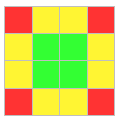
\includegraphics[scale=0.3]{./imgs/dual_min.png}
    \end{textblock*}

\end{frame}

\begin{frame}{Atualização das funções de base}
    As funções de base são atualizadas segundo \citeonline{Zhou2010}: 
    
    % utilizando um valor determinado pelo usuário ($\epsilon$) para verificar a variação da mobilidade de cada fase entre dois passos de tempo consecutivos ($n-1$ e $n$), conforme a seguinte equação:

\begin{equation}
    \dfrac{1}{1+\epsilon} < \dfrac{\mobility_{\phase}^{n}}{\mobility_{\phase}^{n-1}}  < 1 + \epsilon  
    \label{eq:update_bf.1}
\end{equation}
\end{frame}

\begin{frame}{Método de solução da pressão e composições}

    \begin{itemize}
        \justifying
        \item<1-> O cálculo da pressão é realizada de acordo com \citeonline{Zhou2012} (\textit{Two Stage Algebraic Multiscale Solver});
        \item<2-> Solução explícita do transporte resolvida na malha fina. 
    \end{itemize}
    
\end{frame}

\newcounter{problem}
\renewcommand*{\theproblem}{%
    \arabic{problem}%
}

\section{Resultados}

\refstepcounter{problem}
\subsection{Problema \theproblem}
\begin{frame}{Problema \theproblem: Escoamento bidimensional bifásico}

    \begin{itemize}
        \item 80x80 volumes
        \item Dimensão de $0.00762m$ nas direções x e y.
        % \item pressão (P) prescrita no último volume de $13,79MPa$
        % \item vazão (Q) prescrita de injeção de água de $ 3,277 \times 10^{-8} \nicefrac{m^{3}}{s}$ no primeiro volume. 
        \item Campo de permeabilidade homogêneo no valor de $4,9346 10^{-13} m^{2}$.
        \item Foram aplicadas as razões de engrossamento de 7 e 5.
    \end{itemize}
    
    \vspace*{5cm}
    % cfl: 0.9
    % dx: 0.00762 , dy: 0.00762, dz: 0.03048

    \begin{textblock*}{6cm}(0.5cm,5cm) % {block width} 
        \small
    \begin{table}[!ht]
        \centering
        \begin{subtable}{\textwidth}
            \centering
            \begin{tabular}{|c|c|c|c|}
                \hline
                Massa molar $[\nicefrac{g}{mol}]$ & $142,276$ \\
                \hline
                $\criticalT [K]$ & $619,27 $\\
                \hline
                $\criticalP[MPa]$ & $2,109$\\
                \hline
                Acentricidade & $0,489$\\
                \hline
                $\criticalV [\nicefrac{m^{3}}{mol} \times 10^{-4}]$ & $6,03$\\
                \hline            
            \end{tabular}

            \vspace{0.3cm}

            {\small Dados do componente hidrocarboneto}
            \label{tab:table_prob4.c}
        \end{subtable}
    \end{table}
    \end{textblock*}

    \begin{textblock*}{6cm}(7cm,4.8cm)
        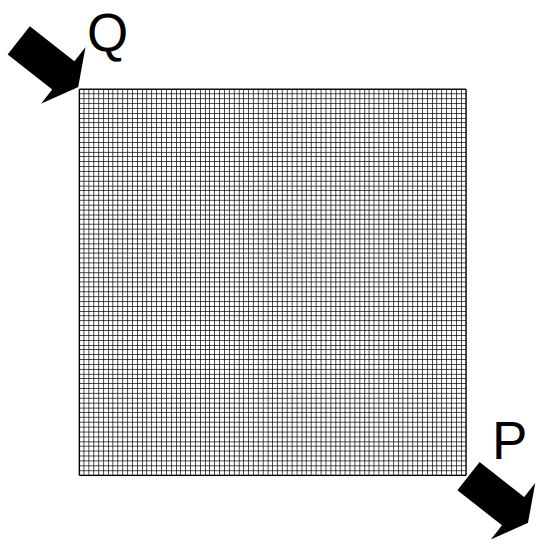
\includegraphics[scale=0.2]{./imgs/prescricao.png}

    \end{textblock*}

    \begin{textblock*}{6cm}(8cm,4.8cm)
        \footnotesize
        $ 3,277 \times 10^{-8} \nicefrac{m^{3}}{s}$

    \end{textblock*}

    \begin{textblock*}{6cm}(10.8cm,7.8cm)
        \footnotesize
        $13,79MPa$

    \end{textblock*}



    
\end{frame}

\begin{frame}{Problema \theproblem}
    \fboxrule=0pt
\renewcommand{\arraystretch}{1.2}
\setlength{\tabcolsep}{5pt}
\setlength{\extrarowheight}{2pt}
\begin{table}[!ht]
    \small
    \centering
    \begin{subtable}[t]{0.48\textwidth}
        \centering
        \begin{tabular}{|c|c|}
            \hline
            $\Saturation_{\oilPhase r \waterPhase}$ & $0,35$ \\
            \hline
            $\Saturation_{\waterPhase r}$ & $0,2$ \\
            \hline
            $k_{r \waterPhase}^{0}$ & $0,2$ \\
            \hline
            $k_{r \oilPhase \waterPhase}^{0}$ & $1$ \\
            \hline
            $e_{\waterPhase}$ & $2$ \\
            \hline
            $e_{\oilPhase \waterPhase}$ & $2$ \\
            \hline
        \end{tabular}
        \caption{Permeabilidade relativa}
    \end{subtable}
    \hspace{\fill}
    \begin{subtable}{0.48\textwidth}
        \centering
        \begin{tabular}{|c|c|}
            \hline
            Pressão inicial & $13,79MPa$ \\
            \hline
            $\Saturation_{\waterPhase}^{0}$ & $0,2$ \\
            \hline
            $\porosidade$ & 0,2 \\
            \hline
            $\temperature$ & $288,7 K$ \\
            \hline
        \end{tabular}
        \caption{Condições Iniciais}
        \label{tab:table_prob4.b}
    \end{subtable}
\end{table}
% \begin{table}[!ht]
%     \centering
%     \caption{Dados do Problema \theproblem}
%     \begin{subtable}[t]{0.48\textwidth}
%         \centering
%         \begin{tabular}{|c|c|}
%             \hline
%             $\Saturation_{\oilPhase r \waterPhase}$ & $0,35$ \\
%             \hline
%             $\Saturation_{\waterPhase r}$ & $0,2$ \\
%             \hline
%             $k_{r \waterPhase}^{0}$ & $0,2$ \\
%             \hline
%             $k_{r \oilPhase \waterPhase}^{0}$ & $1$ \\
%             \hline
%             $e_{\waterPhase}$ & $2$ \\
%             \hline
%             $e_{\oilPhase \waterPhase}$ & $2$ \\
%             \hline
%         \end{tabular}
%         \caption{Permeabilidade relativa}
%         \label{tab:table_prob4.a}
%     \end{subtable}
%     \hspace{\fill}
%     \begin{subtable}{0.48\textwidth}
%         \centering
%         \begin{tabular}{|c|c|}
%             \hline
%             Pressão inicial & $13,79MPa$ \\
%             \hline
%             $\Saturation_{\waterPhase}^{0}$ & $0,2$ \\
%             \hline
%             $\porosidade$ & 0,2 \\
%             \hline
%             $\temperature$ & $288,7 K$ \\
%             \hline
%         \end{tabular}
%         \caption{Condições Iniciais}
%         \label{tab:table_prob4.b}
%     \end{subtable}
%     \bigskip
%     \centering
%     \begin{subtable}{\textwidth}
%         \centering
%         \begin{tabular}{|c|c|c|c|}
%             \hline
%             Massa molar $[\nicefrac{g}{mol}]$ & $142,276$ \\
%             \hline
%             $\criticalT [K]$ & $619,27 $\\
%             \hline
%             $\criticalP[MPa]$ & $2,109$\\
%             \hline
%             Acentricidade & $0,489$\\
%             \hline
%             $\criticalV [\nicefrac{m^{3}}{mol} \times 10^{-4}]$ & $6,03$\\
%             \hline            
%         \end{tabular}
%         \caption{Dados do componente hidrocarboneto}
%         \label{tab:table_prob4.c}
%     \end{subtable}
%     \legend{Elaborado pelo autor}
%     \label{tab:table_prob4}
% \end{table}
\end{frame}
% \setcounter{table}{2}
% \begin{frame}{Problema \theproblem}

%     \begin{columns}
%         \begin{column}{0.5\textwidth}
%             \small
%     \begin{table}[!ht]
%         \centering
%         \begin{subtable}{\textwidth}
%             \centering
%             \begin{tabular}{|c|c|c|c|}
%                 \hline
%                 Massa molar $[\nicefrac{g}{mol}]$ & $142,276$ \\
%                 \hline
%                 $\criticalT [K]$ & $619,27 $\\
%                 \hline
%                 $\criticalP[MPa]$ & $2,109$\\
%                 \hline
%                 Acentricidade & $0,489$\\
%                 \hline
%                 $\criticalV [\nicefrac{m^{3}}{mol} \times 10^{-4}]$ & $6,03$\\
%                 \hline            
%             \end{tabular}

%             \vspace{0.3cm}

%             {\small Dados do componente hidrocarboneto}
%             \label{tab:table_prob4.c}
%         \end{subtable}
%     \end{table}
%         \end{column}
%         \begin{column}{0.5\textwidth}
%             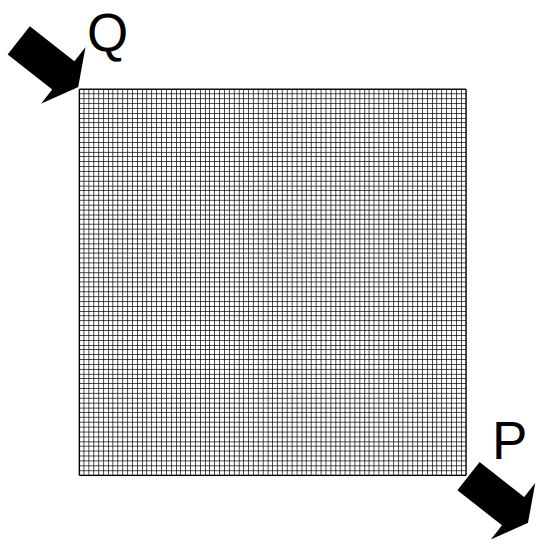
\includegraphics[scale=0.25]{./imgs/prescricao.png}

%             {\small \hspace{0.5cm}Localização das prescrições}
%         \end{column}
%     \end{columns}

    
% \end{frame}

\newcommand{\FrameProblemName}{Problema \theproblem}
% \begin{frame}{\FrameProblemName}
%     \begin{figure}
%         \centering
%         % \caption{Localização das prescrições}
%         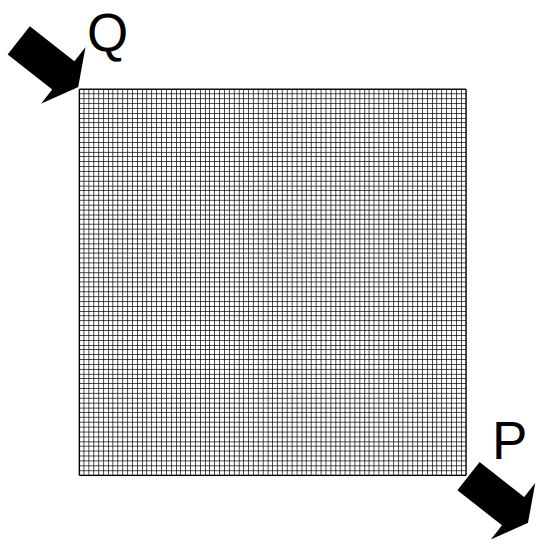
\includegraphics[scale=0.25]{./imgs/prescricao.png}

%         {\small Localização das perscrições}
%         \label{fig:fig3_pr4}
%     \end{figure}
% \end{frame}

\begin{frame}{\FrameProblemName: {\small Malha grossa dual}}
    \begin{figure}
        % \caption{Malha dual}
        \centering
        \begin{subfigure}{.48\textwidth}
            \centering
            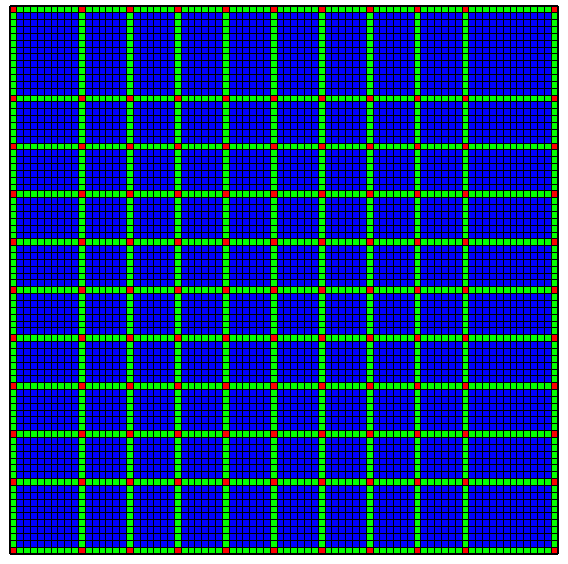
\includegraphics[scale=0.25]{imgs/dual_pr4_cr7.png}
            \caption{Malha dual para Cr = 7}
        \end{subfigure}
        \hspace{\fill}
        \begin{subfigure}{.48\textwidth}
            \centering
            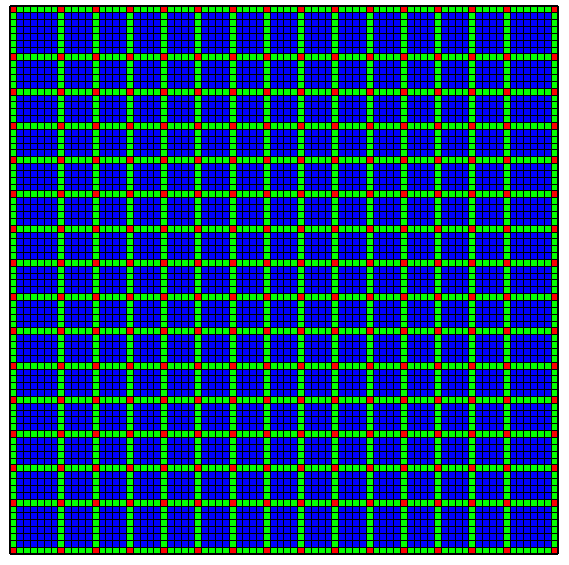
\includegraphics[scale=0.25]{imgs/dual_pr4_cr5.png}
            \caption{Malha dual para Cr = 5}
        \end{subfigure}
    \end{figure}
\end{frame}

\begin{frame}{\FrameProblemName: {\small Tempos de simulação}}
    \begin{figure}[!htbp]
        \centering
        % \caption{Tempos de simulação}
        \begin{subfigure}{.48\textwidth}
            \centering
            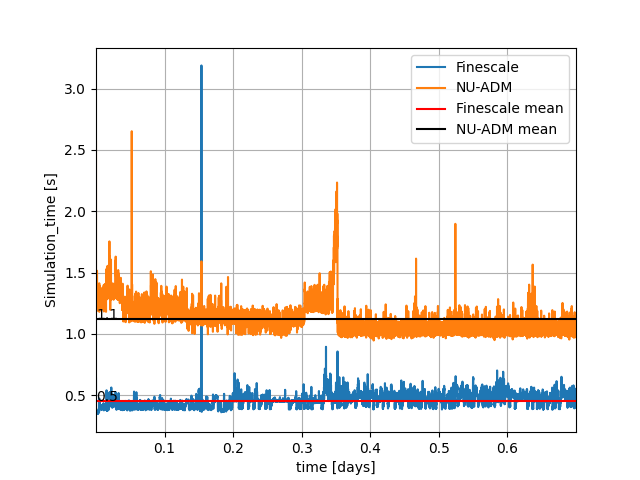
\includegraphics[height=2.5cm]{./imgs/pr4/tempo_sim_cr7.png}
            \caption{Tempo de simulação Cr=7.}
        \end{subfigure}
        \hfill
        \begin{subfigure}{.48\textwidth}
            \centering
            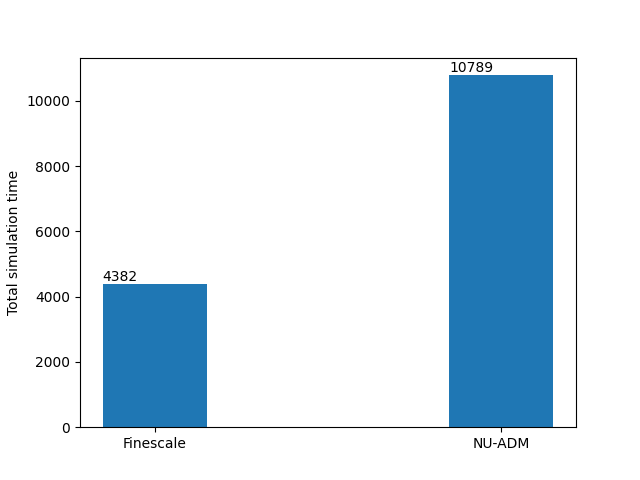
\includegraphics[height=2.5cm]{./imgs/pr4/total_time_cr7.png}
            \caption{Tempo total de simulação Cr=7.}
        \end{subfigure}
        \bigskip
        \begin{subfigure}{.48\textwidth}
            \centering
            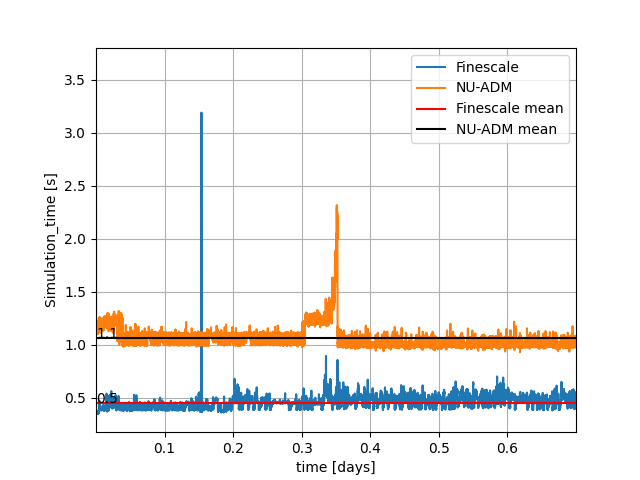
\includegraphics[height=2.5cm]{./imgs/pr4/tempo_sim_cr5.png}
            \caption{Tempo de simulação Cr=5.}
        \end{subfigure}
        \hfill
        \begin{subfigure}{.48\textwidth}
            \centering
            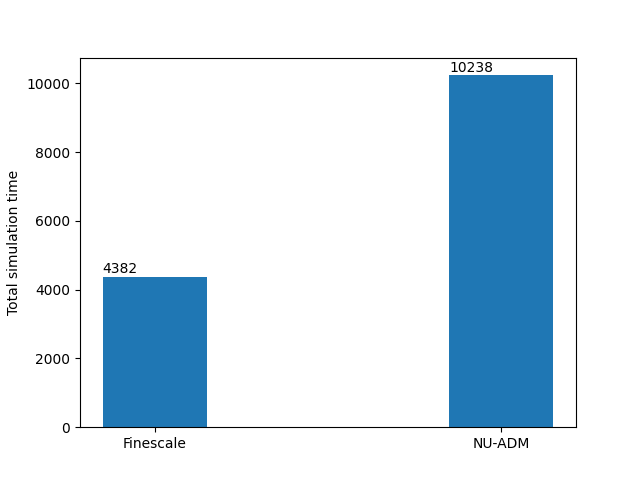
\includegraphics[height=2.5cm]{./imgs/pr4/total_time_cr5.png}
            \caption{Tempo total de simulação Cr=5.}
        \end{subfigure}
        \label{fig:fig4_pr4}
    \end{figure}
\end{frame}

% \begin{frame}{\FrameProblemName}
%     \begin{figure}[!htbp]
%         \centering
%         \caption{Tempos de simulação}
%         % \begin{subfigure}{.48\textwidth}
%         %     \centering
%         %     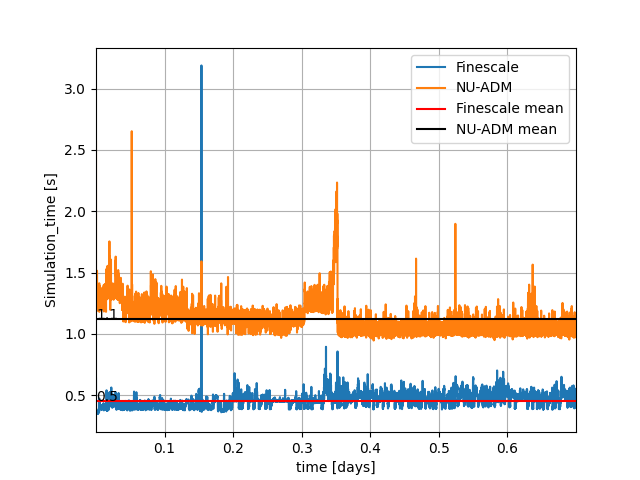
\includegraphics[scale=0.4]{./imgs/pr4/tempo_sim_cr7.png}
%         %     \caption{Tempo de simulação Cr=7.}
%         % \end{subfigure}
%         % \hfill
%         % \begin{subfigure}{.48\textwidth}
%         %     \centering
%         %     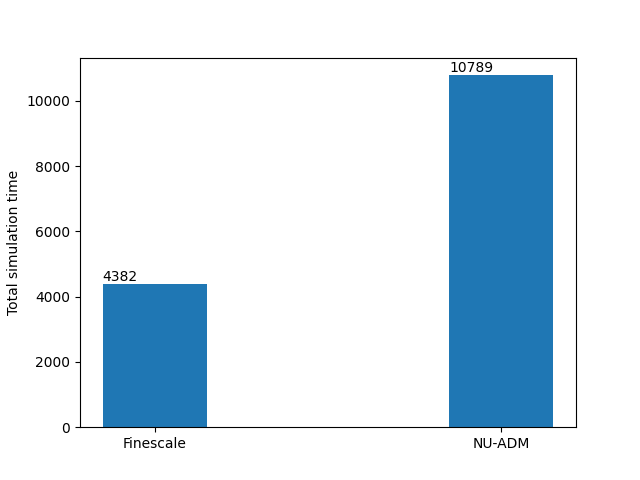
\includegraphics[scale=0.4]{./imgs/pr4/total_time_cr7.png}
%         %     \caption{Tempo total de simulação Cr=7.}
%         % \end{subfigure}
%         % \bigskip
%         \begin{subfigure}{.48\textwidth}
%             \centering
%             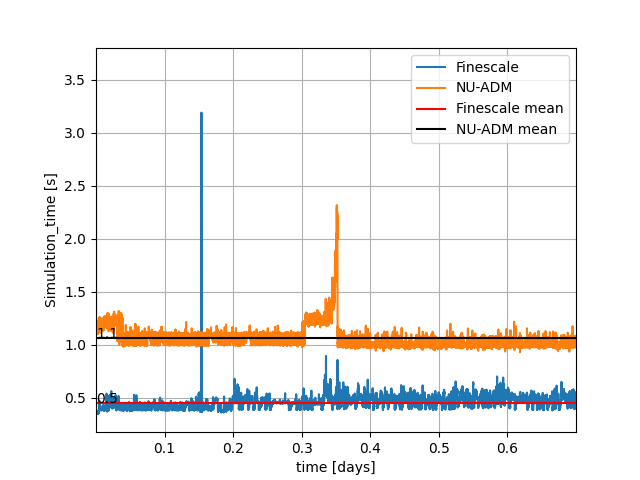
\includegraphics[scale=0.4]{./imgs/pr4/tempo_sim_cr5.png}
%             \caption{Tempo de simulação Cr=5.}
%         \end{subfigure}
%         \hfill
%         \begin{subfigure}{.48\textwidth}
%             \centering
%             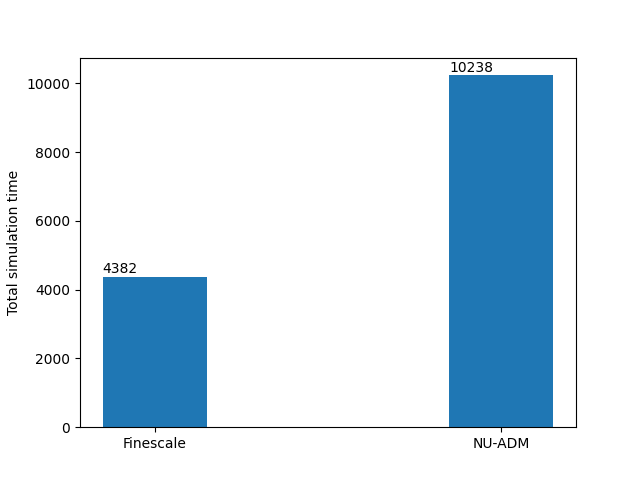
\includegraphics[scale=0.4]{./imgs/pr4/total_time_cr5.png}
%             \caption{Tempo total de simulação Cr=5.}
%         \end{subfigure}
%         \label{fig:fig4.2_pr4}
%     \end{figure}
% \end{frame}

\begin{frame}{\FrameProblemName}
    \begin{figure}[!htbp]
        \centering
        % \caption{Curvas de produção.}
        \begin{subfigure}{.48\textwidth}
            \centering
            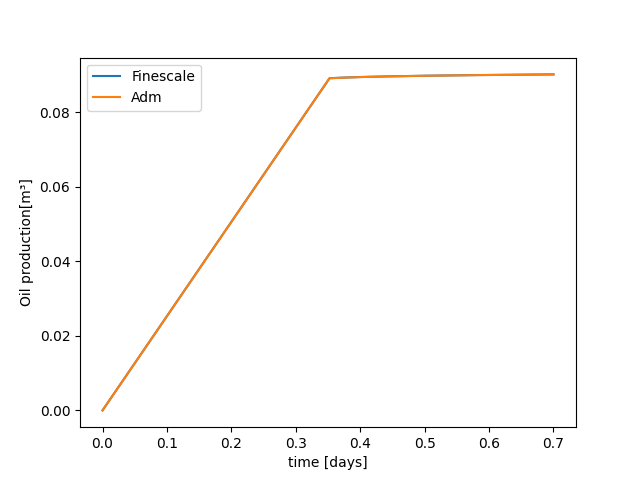
\includegraphics[height=2.5cm]{./imgs/pr4/oil_prod_cr7.png}
            \caption{Curva de produção Cr=7.}
        \end{subfigure}
        \hfill
        \begin{subfigure}{.48\textwidth}
            \centering
            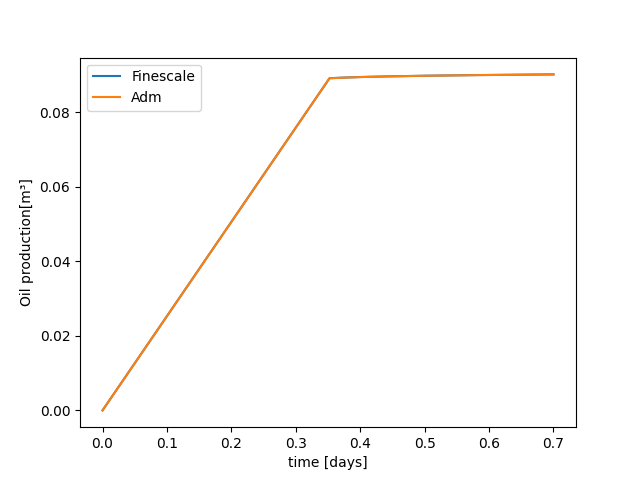
\includegraphics[height=2.5cm]{./imgs/pr4/oil_prod_cr5.png}
            \caption{Curva de produção Cr=5.}
        \end{subfigure}
        \bigskip
        \begin{subfigure}{.48\textwidth}
            \centering
            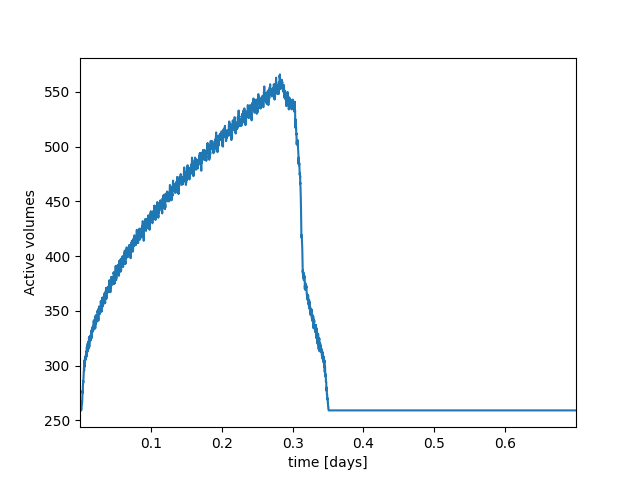
\includegraphics[height=2.5cm]{./imgs/pr4/active_vols_cr7.png}
            \caption{Volumes ativos Cr=7.}
        \end{subfigure}
        \hfill
        \begin{subfigure}{.48\textwidth}
            \centering
            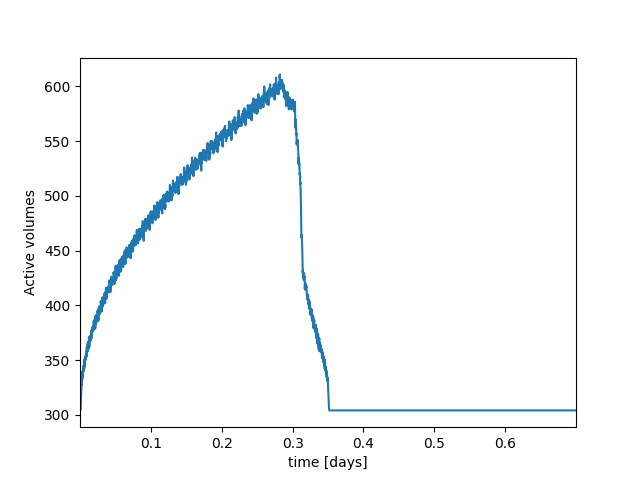
\includegraphics[height=2.5cm]{./imgs/pr4/active_vols_cr5.png}
            \caption{Volumes ativos Cr=5.}
        \end{subfigure}
        \label{fig:fig5_pr4}
    \end{figure}
\end{frame}

% \begin{frame}{\FrameProblemName}
%     \begin{figure}[!htbp]
%         \centering
%         \caption{Volumes Ativos.}
%         \begin{subfigure}{.48\textwidth}
%             \centering
%             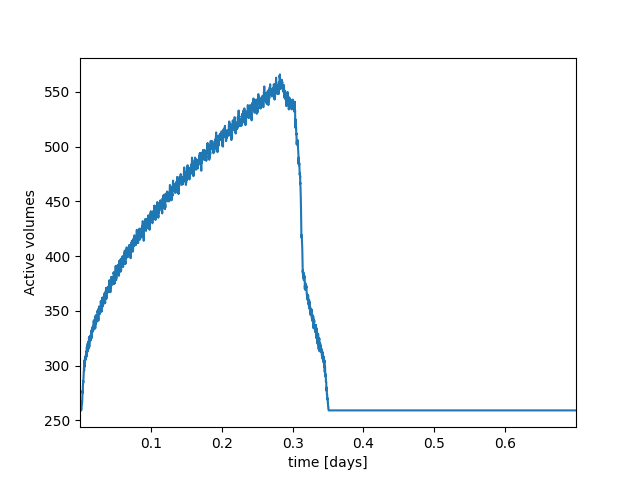
\includegraphics[scale=0.4]{./imgs/pr4/active_vols_cr7.png}
%             \caption{Cr=7.}
%         \end{subfigure}
%         \hfill
%         \begin{subfigure}{.48\textwidth}
%             \centering
%             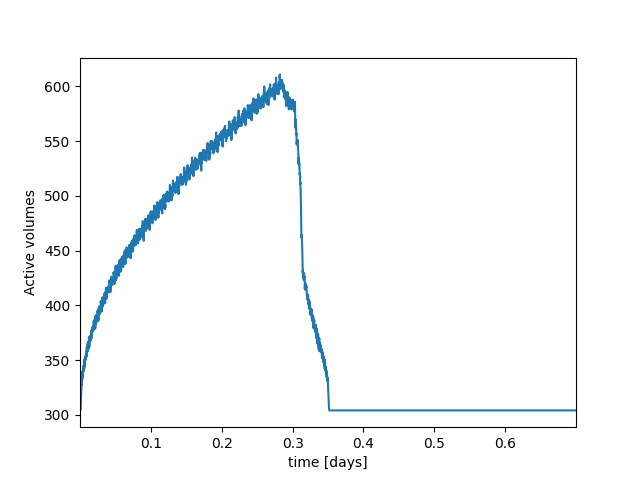
\includegraphics[scale=0.4]{./imgs/pr4/active_vols_cr5.png}
%             \caption{Cr=5.}
%         \end{subfigure}
    
%         % \legend{Fonte: Elaborado pelo autor.}
%         \label{fig:fig6_pr4}
%     \end{figure}
% \end{frame}

\begin{frame}{\FrameProblemName: {\small Malha NU-ADM}}
    \begin{figure}[!htbp]
        \centering
        % \caption{Malha NU-ADM}
        \begin{subfigure}{.48\textwidth}
            \centering
            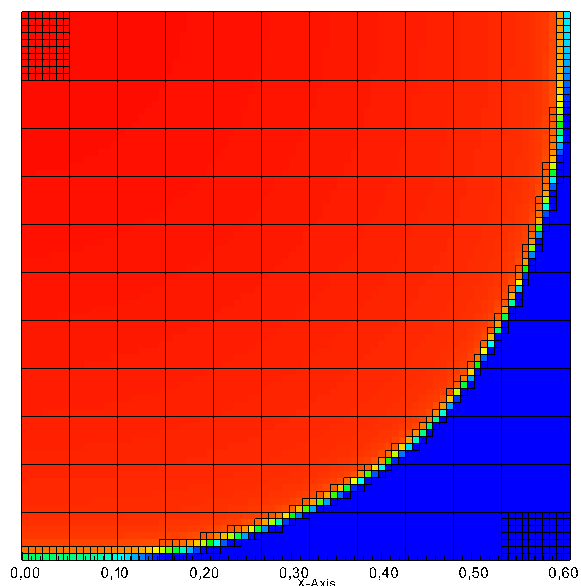
\includegraphics[height=2.5cm]{./imgs/pr4/sat_cr7.png}
            \caption{Saturação de água Cr=7. Vermelho = 0,65, Azul = 0,2}
        \end{subfigure}
        \hfill
        \begin{subfigure}{.48\textwidth}
            \centering
            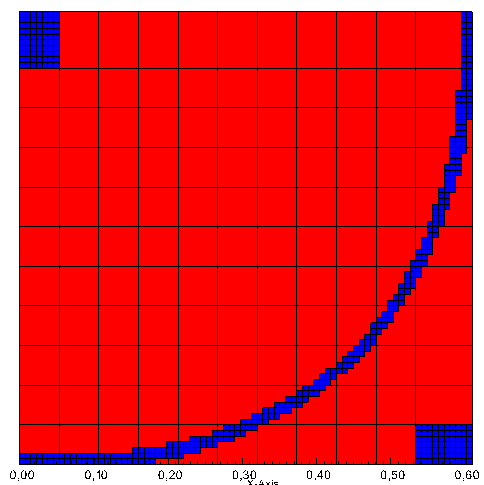
\includegraphics[height=2.5cm]{./imgs/pr4/nivel_cr7.png}
            \caption{Nível Cr=7. Azul=0, Vermelho=1}
        \end{subfigure}
        \bigskip
        \begin{subfigure}{.48\textwidth}
            \centering
            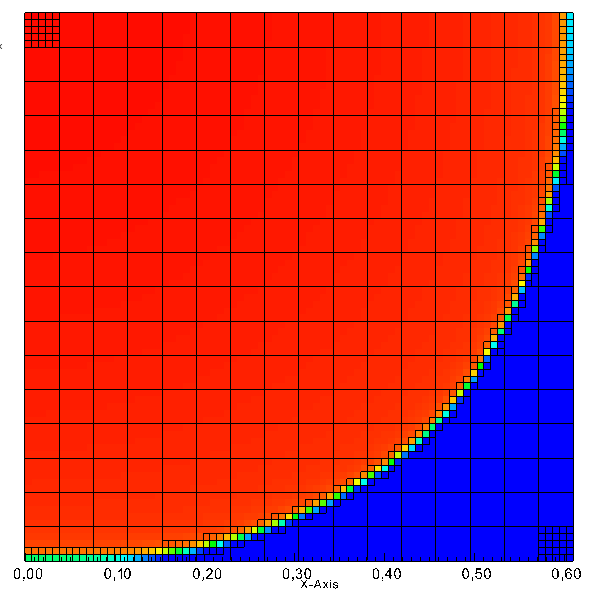
\includegraphics[height=2.5cm]{./imgs/pr4/sat_cr5.png}
            \caption{Saturação de água Cr=5. Vermelho = 0,65, Azul = 0,2}
        \end{subfigure}
        \hfill
        \begin{subfigure}{.48\textwidth}
            \centering
            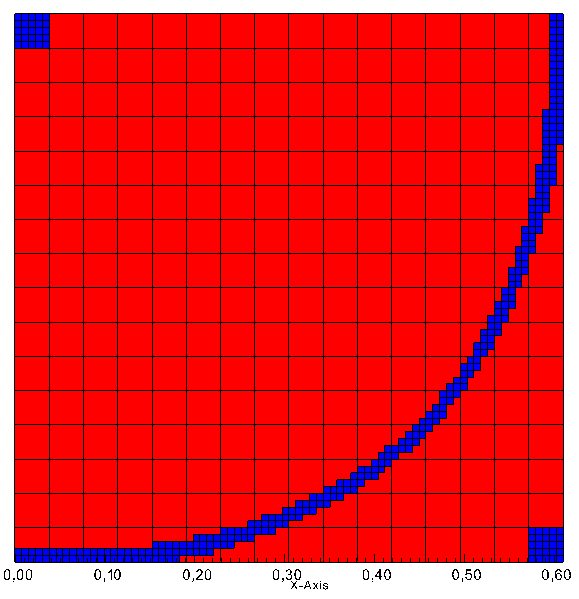
\includegraphics[height=2.5cm]{./imgs/pr4/nivel_cr5.png}
            \caption{Nível Cr=5. Azul=0, Vermelho=1}
        \end{subfigure}
    
        % \legend{Fonte: Elaborado pelo autor.}
        \label{fig:fig7_pr4}
    \end{figure}
\end{frame}

% \begin{frame}{\FrameProblemName}
%     \begin{figure}[!htbp]
%         \centering
%         \caption{Malha NU-ADM}
%         % \begin{subfigure}{.48\textwidth}
%         %     \centering
%         %     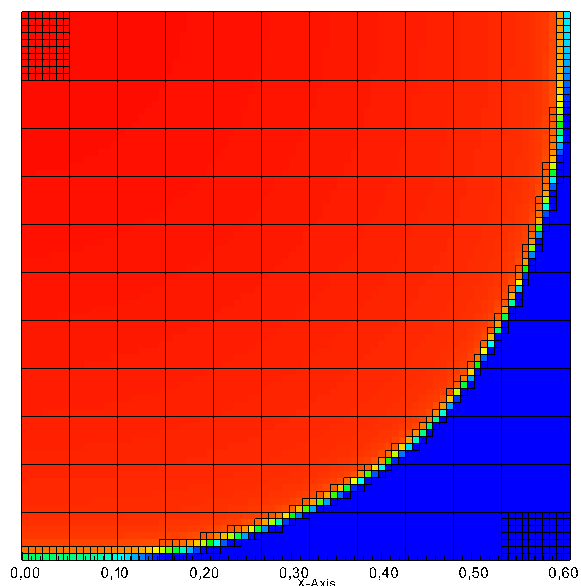
\includegraphics[height=4.6cm]{./imgs/pr4/sat_cr7.png}
%         %     \caption{Saturação de água Cr=7. Vermelho = 0,65, Azul = 0,2}
%         % \end{subfigure}
%         % \hfill
%         % \begin{subfigure}{.48\textwidth}
%         %     \centering
%         %     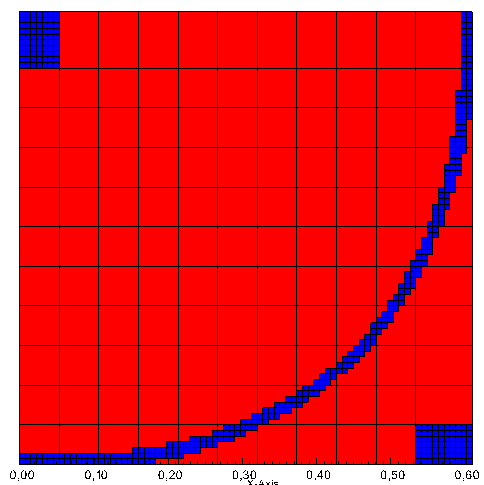
\includegraphics[height=4.7cm]{./imgs/pr4/nivel_cr7.png}
%         %     \caption{Nível Cr=7. Azul=0, Vermelho=1}
%         % \end{subfigure}
%         % \bigskip
%         \begin{subfigure}{.48\textwidth}
%             \centering
%             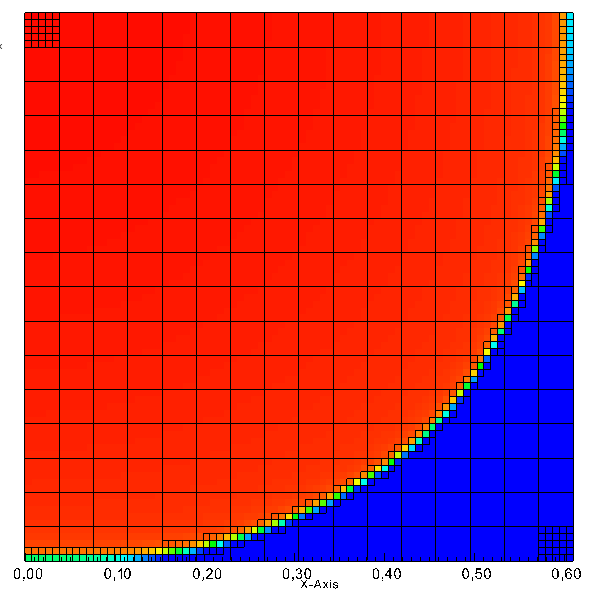
\includegraphics[height=4.6cm]{./imgs/pr4/sat_cr5.png}
%             \caption{Saturação de água Cr=5. Vermelho = 0,65, Azul = 0,2}
%         \end{subfigure}
%         \hfill
%         \begin{subfigure}{.48\textwidth}
%             \centering
%             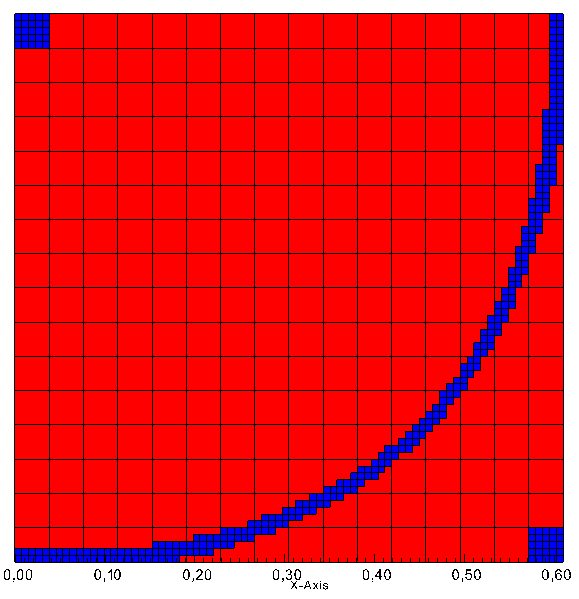
\includegraphics[height=4.7cm]{./imgs/pr4/nivel_cr5.png}
%             \caption{Nível Cr=5. Azul=0, Vermelho=1}
%         \end{subfigure}
    
%         % \legend{Fonte: Elaborado pelo autor.}
%         \label{fig:fig7_pr4}
%     \end{figure}
% \end{frame}

\refstepcounter{problem}
\subsection{Problema \theproblem}

\begin{frame}{\FrameProblemName}

    \begin{itemize}
        \item Escoamento trifásico, 1D, com 6 componentes hidrocarbonetos. 
        \item A malha possui 512 volumes;
        \item Dimensão de cada volume de $5,334375 m$ na direção x
        \item Vazão prescrita de injeção de água no primeiro volume de $4.1377 \times 10^{-4} \nicefrac{m^{3}}{s}$. 
        \item No último volume da malha há pressão Pressão prescrita no último volume de $8, 96MPa$. 
        \item O coeficiente de interação binária entre os componentes é zero.
        \item  Campo de permeabilidade homogêneo no valor de $10^{-14} m^{2}$.
        \item Foram aplicadas as razões de engrossamento 16, 64 e 100. 
    \end{itemize}
    % cfl: 0.5
    % y: 10.66875, z: 10
    
\end{frame}

\begin{frame}{\FrameProblemName}
    \fboxrule=0pt
\renewcommand{\arraystretch}{1.2}
\setlength{\tabcolsep}{5pt}
\setlength{\extrarowheight}{2pt}
\begin{table}[!ht]
    \footnotesize
    \centering
    % \caption{Dados do Problema \theproblem}
    \begin{subtable}[t]{0.48\textwidth}
        \centering
        \begin{tabular}{|c|c|c|c|}
            \hline
            $\Saturation_{\oilPhase r \gasPhase}$ & $0$ & $k_{r \oilPhase \waterPhase}^{0}$ & $0,9$ \\
            \hline
            $\Saturation_{\oilPhase r \waterPhase}$ & $0,1$ & $k_{r \oilPhase \gasPhase}^{0}$ & $0,9$ \\
            \hline
            $\Saturation_{\gasPhase r}$ & 0 & $e_{\waterPhase}$ & $2$ \\
            \hline
            $\Saturation_{\waterPhase r}$ & $0,3$ & $e_{\oilPhase \gasPhase}$ & $2$\\
            \hline
            $k_{r \gasPhase}^{0}$ & $0,9$ & $e_{\oilPhase \waterPhase}$ & $2$\\
            \hline
            $k_{r \waterPhase}^{0}$ & $0,4$ & $e_{\gasPhase}$ & $2$\\
            \hline
        \end{tabular}
        \caption{Permeabilidade relativa}
        \label{tab:table_prob3.a}
    \end{subtable}
    % \hspace{\fill}
    \begin{subtable}{0.48\textwidth}
        \centering
        \begin{tabular}{|c|c|}
            \hline
            Pressão inicial & $10,34MPa$ \\
            \hline
            $\Saturation_{\waterPhase}^{0}$ & 0,3 \\
            \hline
            $\porosidade$ & 0,35 \\
            \hline
            $\temperature$ & $344,25 K$ \\
            \hline
            \rowcolor{gray!40}
            \multicolumn{2}{|Sc|}{ Composição inicial} \\
            \hline
            C1 & $0,5$ \\
            \hline         
            C2 & $0,03$ \\
            \hline         
            C3 & $0,07$ \\       
            \hline  
            C4 & $0,2$ \\       
            \hline  
            C5 & $0,15$ \\       
            \hline  
            C6 & $0,05$ \\       
            \hline  
        \end{tabular}
        \caption{Condições Iniciais}
        \label{tab:table_prob3.b}
    \end{subtable}
    \end{table}
\end{frame}

\begin{frame}{\FrameProblemName}
    \begin{table}
        \small
        \centering
        \begin{subtable}{\textwidth}
            \centering
            \begin{tabular}{|c|c|c|c|c|c|c|}
                \hline
                 & C1 & C2 & C3 & C4 & C5 & C6 \\
                \hline
                Massa molar $[\nicefrac{g}{mol}]$ & $16,042 $ & $44,1$ & $86,178$ & $142,276$ & $212,41$ & $282,5$\\
                \hline
                $\criticalT$ $[K]$ & $190,6 $ & $369,8$ & $507,4$ & $617,6$ & $708$ & $768$\\
                \hline
                $\criticalP$ $[MPa]$ & $4,6$ & $4,24$ & $2,96$ & $2,11$ & $1,47$ & $1,17$\\
                \hline
                Acentricidade & $0,008$ & $0,152$ & $0,299$ & $0,489$ & $0,685$ & $0,912$\\
                \hline
                $\criticalV$ $[\nicefrac{m^{3}}{mol} \times 10^{-4}]$ & $0,99 $ & $2.03$ & $3,7$ & $6,03$ & $8,95$ & $16,9$\\
                \hline            
            \end{tabular}
            \caption{Dados dos componentes}
            \label{tab:table_prob3.c}
        \end{subtable}
    \end{table}
    
\end{frame}

\begin{frame}{\FrameProblemName: {\small Resultados com Cr=64 sem atualizar as funções de base.}}
    \begin{figure}[!ht]
        \centering
        
        \begin{subfigure}{.48\textwidth}
            \centering
            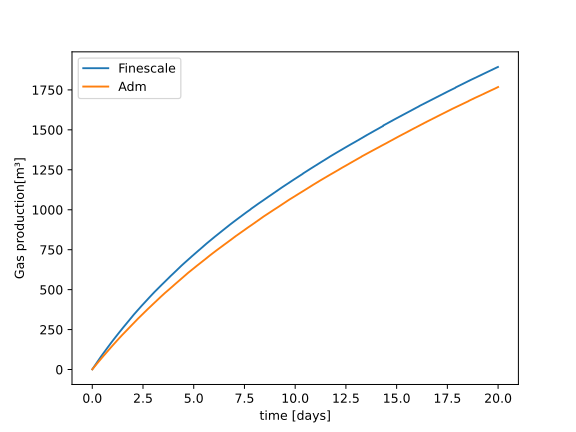
\includegraphics[height=2.5cm]{./imgs/pr3/cr64/no_update/svgtopng/gas_prod.png}
            \caption{Produção de gás}
        \end{subfigure}
        \hfill
        \begin{subfigure}{.48\textwidth}
            \centering
            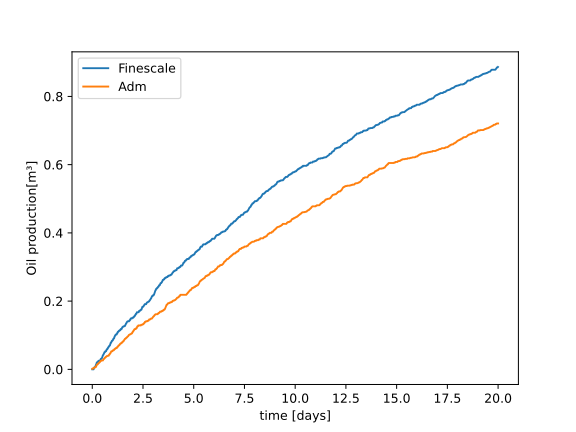
\includegraphics[height=2.5cm]{./imgs/pr3/cr64/no_update/svgtopng/oil_prod.png}
            \caption{Produção de óleo}
        \end{subfigure}
        \bigskip
        \begin{subfigure}{\textwidth}
            \centering
            \includegraphics[height=2.5cm]{./imgs/pr3/cr64/no_update/svgtopng/volumes_ativos.png}
            \caption{Volumes ativos}
        \end{subfigure}
        % \legend{Fonte: Elaborado pelo autor.}
        % \label{fig:fig1_pr3-cr64}
        
    \end{figure}
\end{frame}

\begin{frame}{\FrameProblemName: {\small Resultados com Cr=64 atualizando as funções de base.}}
    \begin{figure}[!ht]
        \centering
        % \caption{Resultados com Cr=64 atualizando as funções de base.}
        \begin{subfigure}{.48\textwidth}
            \centering
            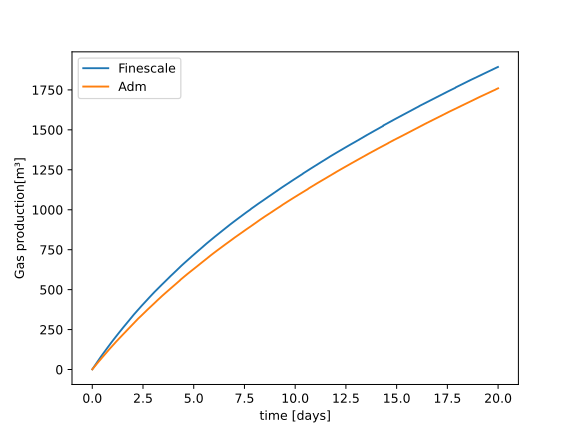
\includegraphics[height=2.5cm]{./imgs/pr3/cr64/update/svgtopng/gas_prod.png}
            \caption{Produção de gás}
        \end{subfigure}
        \hfill
        \begin{subfigure}{.48\textwidth}
            \centering
            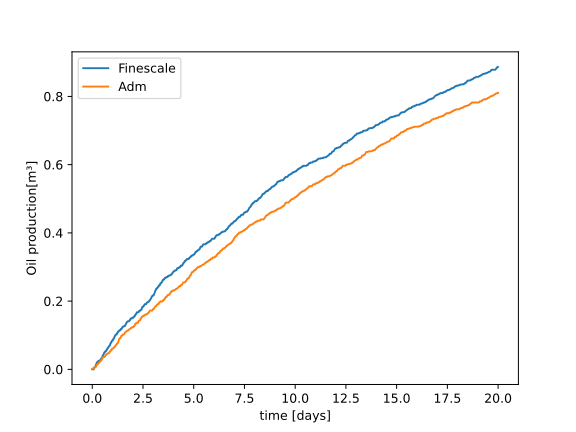
\includegraphics[height=2.5cm]{./imgs/pr3/cr64/update/svgtopng/oil_prod.png}
            \caption{Produção de óleo}
        \end{subfigure}
        \bigskip
        \begin{subfigure}{.48\textwidth}
            \centering
            \includegraphics[height=2.5cm]{./imgs/pr3/cr64/update/svgtopng/volumes_ativos.png}
            \caption{Volumes ativos}
        \end{subfigure}
        \hfill
        \begin{subfigure}{.48\textwidth}
            \centering
            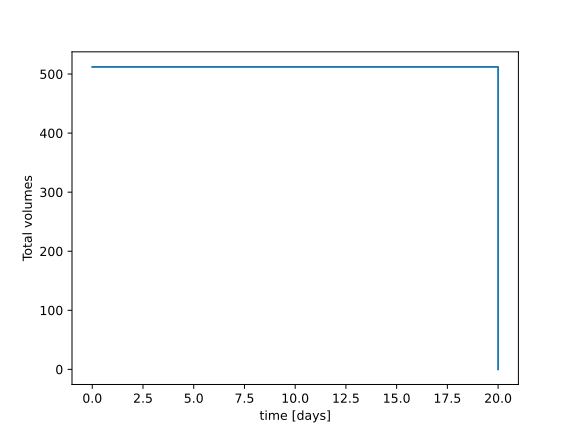
\includegraphics[height=2.5cm]{./imgs/pr3/cr64/update/svgtopng/volumes_update.png}
            \caption{Quantidade de volumes para atualizar as funções de base}
        \end{subfigure}
        % \legend{Fonte: Elaborado pelo autor.}
        \label{fig:fig2_pr3-cr64}
        
    \end{figure}
    
\end{frame}

\begin{frame}{\FrameProblemName: {\small Tempos de simulação com Cr=64.}}
    \begin{figure}[!h]
        \centering
        % \caption{Tempos de simulação com Cr=64.}
        \begin{subfigure}{.48\textwidth}
            \centering
            \includegraphics[height=2.5cm]{./imgs/pr3/cr64/no_update/svgtopng/tempo_simulacao.png}
            \caption{Tempo de simulação sem atualizar as funções de base}
        \end{subfigure}
        \hfill
        \begin{subfigure}{.48\textwidth}
            \centering
            \includegraphics[height=2.5cm]{./imgs/pr3/cr64/no_update/svgtopng/tempo_total.png}
            \caption{Tempo total de simulação sem atualizar as funções de base}
        \end{subfigure}
        \bigskip
        \begin{subfigure}{.48\textwidth}
            \centering
            \includegraphics[height=2.5cm]{./imgs/pr3/cr64/update/svgtopng/tempo_simulacao.png}
            \caption{Tempo de simulação atualizando as funções de base}
        \end{subfigure}
        \hfill
        \begin{subfigure}{.48\textwidth}
            \centering
            \includegraphics[height=2.5cm]{./imgs/pr3/cr64/update/svgtopng/tempo_total.png}
            \caption{Tempo total de simulação atualizando as funções de base}
        \end{subfigure}
        % \legend{Fonte: Elaborado pelo autor.}
        \label{fig:fig3_pr3-cr64}
    \end{figure}
    
\end{frame}

\begin{frame}{\FrameProblemName: {\small Resultados com Cr=16 sem atualizar as funções de base.}}
    \begin{figure}[!ht]
        \centering
        % \caption{Resultados com Cr=16 sem atualizar as funções de base.}
        \begin{subfigure}{.48\textwidth}
            \centering
            \includegraphics[height=2.5cm]{./imgs/pr3/cr16/no_update/gas_prod.png}
            \caption{Produção de gás}
        \end{subfigure}
        \hfill
        \begin{subfigure}{.48\textwidth}
            \centering
            \includegraphics[height=2.5cm]{./imgs/pr3/cr16/no_update/oil_prod.png}
            \caption{Produção de óleo}
        \end{subfigure}
        \bigskip
        \begin{subfigure}{\textwidth}
            \centering
            \includegraphics[height=2.5cm]{./imgs/pr3/cr16/no_update/volumes_ativos.png}
            \caption{Volumes ativos}
        \end{subfigure}
        % \legend{Fonte: Elaborado pelo autor.}
        \label{fig:fig4_pr3-cr16}
        
    \end{figure}
    
\end{frame}

\begin{frame}{\FrameProblemName: {\small Resultados com Cr=16 atualizando as funções de base.}}
    \begin{figure}[!ht]
        \centering
        % \caption{Resultados com Cr=16 atualizando as funções de base.}
        \begin{subfigure}{.48\textwidth}
            \centering
            \includegraphics[height=2.5cm]{./imgs/pr3/cr16/Update/gas_prod.png}
            \caption{Produção de gás}
        \end{subfigure}
        \hfill
        \begin{subfigure}{.48\textwidth}
            \centering
            \includegraphics[height=2.5cm]{./imgs/pr3/cr16/Update/oil_prod.png}
            \caption{Produção de óleo}
        \end{subfigure}
        \bigskip
        \begin{subfigure}{.48\textwidth}
            \centering
            \includegraphics[height=2.5cm]{./imgs/pr3/cr16/Update/volumes_ativos.png}
            \caption{Volumes ativos}
        \end{subfigure}
        \hfill
        \begin{subfigure}{.48\textwidth}
            \centering
            \includegraphics[height=2.5cm]{./imgs/pr3/cr16/Update/volumes_update.png}
            \caption{Quantidade de volumes para atualizar as funções de base}
        \end{subfigure}
        % \legend{Fonte: Elaborado pelo autor.}
        \label{fig:fig5_pr3-cr16}
        
    \end{figure}
\end{frame}

\begin{frame}{\FrameProblemName: {\small Tempos de simulação com Cr=16.}}
    \begin{figure}[!h]
        \centering
        % \caption{Tempos de simulação com Cr=16.}
        \begin{subfigure}{.48\textwidth}
            \centering
            \includegraphics[height=2.5cm]{./imgs/pr3/cr16/no_update/tempo_simulacao.png}
            \caption{Tempo de simulação sem atualizar as funções de base}
        \end{subfigure}
        \hfill
        \begin{subfigure}{.48\textwidth}
            \centering
            \includegraphics[height=2.5cm]{./imgs/pr3/cr16/no_update/tempo_total.png}
            \caption{Tempo total de simulação sem atualizar as funções de base}
        \end{subfigure}
        \bigskip
        \begin{subfigure}{.48\textwidth}
            \centering
            \includegraphics[height=2.5cm]{./imgs/pr3/cr16/Update/tempo_simulacao.png}
            \caption{Tempo de simulação atualizando as funções de base}
        \end{subfigure}
        \hfill
        \begin{subfigure}{.48\textwidth}
            \centering
            \includegraphics[height=2.5cm]{./imgs/pr3/cr16/Update/tempo_total.png}
            \caption{Tempo total de simulação atualizando as funções de base}
        \end{subfigure}
    
        % \legend{Fonte: Elaborado pelo autor.}
        \label{fig:fig6_pr3-cr16}
    \end{figure}
    
\end{frame}

\begin{frame}{\FrameProblemName: {\small Resultados com Cr=100 sem atualizar as funções de base.}}
    \begin{figure}[!ht]
        \centering
        % \caption{Resultados com Cr=100 sem atualizar as funções de base.}
        \begin{subfigure}{.48\textwidth}
            \centering
            \includegraphics[height=2.5cm]{./imgs/pr3/cr100/no_update/svgtopng/gas_prod.png}
            \caption{Produção de gás}
        \end{subfigure}
        \hfill
        \begin{subfigure}{.48\textwidth}
            \centering
            \includegraphics[height=2.5cm]{./imgs/pr3/cr100/no_update/svgtopng/oil_prod.png}
            \caption{Produção de óleo}
        \end{subfigure}
        \bigskip
        \begin{subfigure}{\textwidth}
            \centering
            \includegraphics[height=2.5cm]{./imgs/pr3/cr100/no_update/svgtopng/volumes_ativos.png}
            \caption{Volumes ativos}
        \end{subfigure}
        % \legend{Fonte: Elaborado pelo autor.}
        \label{fig:fig7_pr3-cr100}
        
    \end{figure}
\end{frame}

\begin{frame}{\FrameProblemName: {\small Resultados com Cr=100 atualizando as funções de base.}}
    \begin{figure}[!ht]
        \centering
        % \caption{Resultados com Cr=100 atualizando as funções de base.}
        \begin{subfigure}[t]{.48\textwidth}
            \centering
            \includegraphics[height=2.5cm]{./imgs/pr3/cr100/update/svgtopng/gas_prod.png}
            \caption{Produção de gás}
        \end{subfigure}
        \hfill
        \begin{subfigure}[t]{.48\textwidth}
            \centering
            \includegraphics[height=2.5cm]{./imgs/pr3/cr100/update/svgtopng/oil_prod.png}
            \caption{Produção de óleo}
        \end{subfigure}
        \bigskip
        \begin{subfigure}[t]{.48\textwidth}
            \centering
            \includegraphics[height=2.5cm]{./imgs/pr3/cr100/update/svgtopng/volumes_ativos.png}
            \caption{Volumes ativos}
        \end{subfigure}
        \hfill
        \begin{subfigure}[t]{.48\textwidth}
            \centering
            \includegraphics[height=2.5cm]{./imgs/pr3/cr100/update/svgtopng/n_volumes_update.png}
            \caption{Quantidade de volumes para atualizar as funções de base}
        \end{subfigure}
        % \legend{Fonte: Elaborado pelo autor.}
        \label{fig:fig8_pr3-cr100}
        
    \end{figure}
    
\end{frame}

\begin{frame}{\FrameProblemName: {\small Tempos de simulação com Cr=100.}}
    \begin{figure}[!h]
        \centering
        % \caption{Tempos de simulação com Cr=100.}
        \begin{subfigure}{.48\textwidth}
            \centering
            \includegraphics[height=2.5cm]{./imgs/pr3/cr100/no_update/svgtopng/tempo_de_simulacao.png}
            \caption{Tempo de simulação sem atualizar as funções de base}
        \end{subfigure}
        \hfill
        \begin{subfigure}{.48\textwidth}
            \centering
            \includegraphics[height=2.5cm]{./imgs/pr3/cr100/no_update/svgtopng/tempo_total.png}
            \caption{Tempo total de simulação sem atualizar as funções de base}
        \end{subfigure}
        \bigskip
        \begin{subfigure}[t]{.48\textwidth}
            \centering
            \includegraphics[height=2.5cm]{./imgs/pr3/cr16/Update/tempo_simulacao.png}
            \caption{Tempo de simulação atualizando as funções de base}
        \end{subfigure}
        \hfill
        \begin{subfigure}[t]{.48\textwidth}
            \centering
            \includegraphics[height=2.5cm]{./imgs/pr3/cr16/Update/tempo_total.png}
            \caption{Tempo total de simulação atualizando as funções de base}
        \end{subfigure}
    
        % \legend{Fonte: Elaborado pelo autor.}
        \label{fig:fig9_pr3-cr100}
    \end{figure}
\end{frame}

\refstepcounter{problem}
\subsection{Problema \theproblem}

\begin{frame}{\FrameProblemName}
    \begin{itemize}
        \item Escoamento 1D com 3 componentes hidrocarbonetos e com duas fases (óleo e gás). 
        \item 5000 volumes 
        \item Pressão prescrita no primeiro volume de $7MPa$ e composição prescrita de injeção de $0,9$ do componente C1 e $0,1$ do componente C2. 
        \item Pressão prescrita no último volume de $6MPa$. 
        \item O coeficiente de interação binária entre os componentes é zero 
        \item A dimensão dos volumes na direção x é de $0,01m$. 
        \item Campo de permeabilidade homogêneo no valor de $10^{-15} m^{2}$.
        \item Razões de engrossamento: 20, 50 e 100.
    \end{itemize}
\end{frame}

\begin{frame}{\FrameProblemName: {\small Resultados com Cr=20 sem atualizar as funções de base.}}
    \begin{figure}[!ht]
        \centering
        % \caption{Resultados com Cr=20 sem atualizar as funções de base.}
        \begin{subfigure}{.48\textwidth}
            \centering
            \includegraphics[height=2.5cm]{./imgs/pr2/3k_5000x1x1/cr 20/v2/no_update/svgtopng/figura_case-finescale_3k_5000_CR20_no__updateGas_production.png}
            \caption{Produção de gás}
        \end{subfigure}
        \hfill
        \begin{subfigure}{.48\textwidth}
            \centering
            \includegraphics[height=2.5cm]{./imgs/pr2/3k_5000x1x1/cr 20/v2/no_update/svgtopng/figura_case-finescale_3k_5000_CR20_no__updateOil_production.png}
            \caption{Produção de óleo}
        \end{subfigure}
        \bigskip
        \begin{subfigure}{\textwidth}
            \centering
            \includegraphics[height=2.5cm]{./imgs/pr2/3k_5000x1x1/cr 20/v2/no_update/svgtopng/figura_case-finescale_3k_5000_CR20_no__updateActive_volumes.png}
            \caption{Volumes ativos}
        \end{subfigure}
        % \legend{Fonte: Elaborado pelo autor.}
        \label{fig:fig1_pr2-cr20}
        
    \end{figure}
\end{frame}

\begin{frame}{\FrameProblemName: {\small Resultados com Cr=20 atualizando as funções de base.}}
    \begin{figure}[!ht]
        \centering
        % \caption{Resultados com Cr=20 atualizando as funções de base.}
        \begin{subfigure}{.48\textwidth}
            \centering
            \includegraphics[height=2.5cm   ]{./imgs/pr2/3k_5000x1x1/cr 20/v2/update/svgtopng/figura_case-finescale_3k_5000_CR20_updateGas_production.png}
            \caption{Produção de gás}
        \end{subfigure}
        \hfill
        \begin{subfigure}{.48\textwidth}
            \centering
            \includegraphics[height=2.5cm]{./imgs/pr2/3k_5000x1x1/cr 20/v2/update/svgtopng/figura_case-finescale_3k_5000_CR20_updateOil_production.png}
            \caption{Produção de óleo}
        \end{subfigure}
        \bigskip
        \begin{subfigure}{.48\textwidth}
            \centering
            \includegraphics[height=2.5cm]{./imgs/pr2/3k_5000x1x1/cr 20/v2/update/svgtopng/figura_case-finescale_3k_5000_CR20_updateActive_volumes.png}
            \caption{Volumes ativos}
        \end{subfigure}
        \hfill
        \begin{subfigure}{.48\textwidth}
            \centering
            \includegraphics[height=2.5cm]{./imgs/pr2/3k_5000x1x1/cr 20/v2/update/svgtopng/figura_case-finescale_3k_5000_CR20_updateTotal volumes.png}
            \caption{Quantidade de volumes para atualizar as funções de base}
        \end{subfigure}
        % \legend{Fonte: Elaborado pelo autor.}
        \label{fig:fig2_pr2-cr20}
        
    \end{figure}
\end{frame}

\begin{frame}{\FrameProblemName: {\small Tempos de simulação com Cr=20.}}
    \begin{figure}[!h]
        \centering
        % \caption{Tempos de simulação com Cr=20.}
        \begin{subfigure}{.48\textwidth}
            \centering
            \includegraphics[height=2.5cm]{./imgs/pr2/3k_5000x1x1/cr 20/v2/no_update/svgtopng/figura_case-finescale_3k_5000_CR20_no__updateTempo de simulaçãoActive_volumes.png}
            \caption{Tempo de simulação sem atualizar as funções de base}
        \end{subfigure}
        \hfill
        \begin{subfigure}{.48\textwidth}
            \centering
            \includegraphics[height=2.5cm]{./imgs/pr2/3k_5000x1x1/cr 20/v2/no_update/svgtopng/figura_case-finescale_3k_5000_CR20_no__updateTotal_simulation_time.png}
            \caption{Tempo total de simulação sem atualizar as funções de base}
        \end{subfigure}
        \bigskip
        \begin{subfigure}[t]{.48\textwidth}
            \centering
            \includegraphics[height=2.5cm]{./imgs/pr2/3k_5000x1x1/cr 20/v2/update/svgtopng/figura_case-finescale_3k_5000_CR20_updateTempo de simulaçãoActive_volumes.png}
            \caption{Tempo de simulação atualizando as funções de base}
        \end{subfigure}
        \hfill
        \begin{subfigure}[t]{.48\textwidth}
            \centering
            \includegraphics[height=2.5cm]{./imgs/pr2/3k_5000x1x1/cr 20/v2/update/svgtopng/figura_case-finescale_3k_5000_CR20_updateTotal_simulation_time.png}
            \caption{Tempo total de simulação atualizando as funções de base}
        \end{subfigure}
    
        % \legend{Fonte: Elaborado pelo autor.}
        \label{fig:fig3_pr3-cr20}
    \end{figure}
\end{frame}

\begin{frame}{\FrameProblemName: {\small Resultados com Cr=50 sem atualizar as funções de base.}}
    \begin{figure}[!ht]
        \centering
        % \caption{Resultados com Cr=50 sem atualizar as funções de base.}
        \begin{subfigure}{.48\textwidth}
            \centering
            \includegraphics[height=2.5cm]{./imgs/pr2/3k_5000x1x1/cr 50/v2/no_update/svgtopng/figura_case-finescale_3k_5000_CR50_no_updateGas_production.png}
            \caption{Produção de gás}
        \end{subfigure}
        \hfill
        \begin{subfigure}{.48\textwidth}
            \centering
            \includegraphics[height=2.5cm]{./imgs/pr2/3k_5000x1x1/cr 50/v2/no_update/svgtopng/figura_case-finescale_3k_5000_CR50_no_updateOil_production.png}
            \caption{Produção de óleo}
        \end{subfigure}
        \bigskip
        \begin{subfigure}{\textwidth}
            \centering
            \includegraphics[height=2.5cm]{./imgs/pr2/3k_5000x1x1/cr 50/v2/no_update/svgtopng/figura_case-finescale_3k_5000_CR50_no_updateActive_volumes.png}
            \caption{Volumes ativos}
        \end{subfigure}
        % \legend{Fonte: Elaborado pelo autor.}
        \label{fig:fig4_pr2-cr50}
        
    \end{figure}
    
\end{frame}

\begin{frame}{\FrameProblemName: {\small Resultados com Cr=50 atualizando as funções de base.}}
    \begin{figure}[!ht]
        \centering
        % \caption{Resultados com Cr=50 atualizando as funções de base.}
        \begin{subfigure}{.48\textwidth}
            \centering
            \includegraphics[height=2.5cm]{./imgs/pr2/3k_5000x1x1/cr 50/v2/update/svgtopng/figura_case-finescale_3k_5000_CR50_updateGas_production.png}
            \caption{Produção de gás}
        \end{subfigure}
        \hfill
        \begin{subfigure}{.48\textwidth}
            \centering
            \includegraphics[height=2.5cm]{./imgs/pr2/3k_5000x1x1/cr 50/v2/update/svgtopng/figura_case-finescale_3k_5000_CR50_updateOil_production.png}
            \caption{Produção de óleo}
        \end{subfigure}
        \bigskip
        \begin{subfigure}{.48\textwidth}
            \centering
            \includegraphics[height=2.5cm]{./imgs/pr2/3k_5000x1x1/cr 50/v2/update/svgtopng/figura_case-finescale_3k_5000_CR50_updateActive_volumes.png}
            \caption{Volumes ativos}
        \end{subfigure}
        \hfill
        \begin{subfigure}{.48\textwidth}
            \centering
            \includegraphics[height=2.5cm]{./imgs/pr2/3k_5000x1x1/cr 50/v2/update/svgtopng/figura_case-finescale_3k_5000_CR50_updateTotal volumes.png}
            \caption{Quantidade de volumes para atualizar as funções de base}
        \end{subfigure}
        % \legend{Fonte: Elaborado pelo autor.}
        \label{fig:fig5_pr2-cr50}
        
    \end{figure}
\end{frame}

\begin{frame}{\FrameProblemName: {\small Tempos de simulação com Cr=50.}}
    \begin{figure}[!h]
        \centering
        % \caption{Tempos de simulação com Cr=50.}
        \begin{subfigure}{.48\textwidth}
            \centering
            \includegraphics[height=2.5cm]{./imgs/pr2/3k_5000x1x1/cr 50/v2/no_update/svgtopng/figura_case-finescale_3k_5000_CR50_no_updateTempo de simulaçãoActive_volumes.png}
            \caption{Tempo de simulação sem atualizar as funções de base}
        \end{subfigure}
        \hfill
        \begin{subfigure}{.48\textwidth}
            \centering
            \includegraphics[height=2.5cm]{./imgs/pr2/3k_5000x1x1/cr 50/v2/no_update/svgtopng/figura_case-finescale_3k_5000_CR50_no_updateTotal_simulation_time.png}
            \caption{Tempo total de simulação sem atualizar as funções de base}
        \end{subfigure}
        \bigskip
        \begin{subfigure}[t]{.48\textwidth}
            \centering
            \includegraphics[height=2.5cm]{./imgs/pr2/3k_5000x1x1/cr 50/v2/update/svgtopng/figura_case-finescale_3k_5000_CR50_updateTempo de simulaçãoActive_volumes.png}
            \caption{Tempo de simulação atualizando as funções de base}
        \end{subfigure}
        \hfill
        \begin{subfigure}[t]{.48\textwidth}
            \centering
            \includegraphics[height=2.5cm]{./imgs/pr2/3k_5000x1x1/cr 50/v2/update/svgtopng/figura_case-finescale_3k_5000_CR50_updateTotal_simulation_time.png}
            \caption{Tempo total de simulação atualizando as funções de base}
        \end{subfigure}
    
        % \legend{Fonte: Elaborado pelo autor.}
        \label{fig:fig6_pr2-cr50}
    \end{figure}
\end{frame}

\begin{frame}{\FrameProblemName: {\small Resultados com Cr=100 sem atualizar as funções de base.}}
    \begin{figure}[!ht]
        \centering
        % \caption{Resultados com Cr=100 sem atualizar as funções de base.}
        \begin{subfigure}{.48\textwidth}
            \centering
            \includegraphics[height=2.5cm]{./imgs/pr2/3k_5000x1x1/cr 100/3k_5000_cr100_no_update/svgtopng/figura_case-finescale_3k_5000_CR100_no_updateGas_production.png}
            \caption{Produção de gás}
        \end{subfigure}
        \hfill
        \begin{subfigure}{.48\textwidth}
            \centering
            \includegraphics[height=2.5cm]{./imgs/pr2/3k_5000x1x1/cr 100/3k_5000_cr100_no_update/svgtopng/figura_case-finescale_3k_5000_CR100_no_updateOil_production.png}
            \caption{Produção de óleo}
        \end{subfigure}
        \bigskip
        \begin{subfigure}{\textwidth}
            \centering
            \includegraphics[height=2.5cm]{./imgs/pr2/3k_5000x1x1/cr 100/3k_5000_cr100_no_update/svgtopng/figura_case-finescale_3k_5000_CR100_no_updateActive_volumes.png}
            \caption{Volumes ativos}
        \end{subfigure}
        % \legend{Fonte: Elaborado pelo autor.}
        \label{fig:fig7_pr2-cr100}
        
    \end{figure}
\end{frame}

\begin{frame}{\FrameProblemName: {\small Resultados com Cr=100 atualizando as funções de base.}}
    \begin{figure}[!ht]
        \centering
        % \caption{Resultados com Cr=100 atualizando as funções de base.}
        \begin{subfigure}{.48\textwidth}
            \centering
            \includegraphics[height=2.5cm]{./imgs/pr2/3k_5000x1x1/cr 100/3k_5000_cr100_update/svgtopng/figura_case-finescale_3k_5000_CR100_updateGas_production.png}
            \caption{Produção de gás}
        \end{subfigure}
        \hfill
        \begin{subfigure}{.48\textwidth}
            \centering
            \includegraphics[height=2.5cm]{./imgs/pr2/3k_5000x1x1/cr 100/3k_5000_cr100_update/svgtopng/figura_case-finescale_3k_5000_CR100_updateOil_production.png}
            \caption{Produção de óleo}
        \end{subfigure}
        \bigskip
        \begin{subfigure}{.48\textwidth}
            \centering
            \includegraphics[height=2.5cm]{./imgs/pr2/3k_5000x1x1/cr 100/3k_5000_cr100_update/svgtopng/figura_case-finescale_3k_5000_CR100_updateActive_volumes.png}
            \caption{Volumes ativos}
        \end{subfigure}
        \hfill
        \begin{subfigure}{.48\textwidth}
            \centering
            \includegraphics[height=2.5cm]{./imgs/pr2/3k_5000x1x1/cr 100/3k_5000_cr100_update/svgtopng/figura_case-finescale_3k_5000_CR100_updateTotal volumes.png}
            \caption{Quantidade de volumes para atualizar as funções de base}
        \end{subfigure}
        % \legend{Fonte: Elaborado pelo autor.}
        \label{fig:fig8_pr2-cr100}
        
    \end{figure}
\end{frame}

\begin{frame}{\FrameProblemName: {\small Tempos de simulação com Cr=100.}}
    \begin{figure}[!h]
        \centering
        % \caption{Tempos de simulação com Cr=100.}
        \begin{subfigure}{.48\textwidth}
            \centering
            \includegraphics[height=2.5cm]{./imgs/pr2/3k_5000x1x1/cr 100/3k_5000_cr100_no_update/svgtopng/figura_case-finescale_3k_5000_CR100_no_updateTempo de simulaçãoActive_volumes.png}
            \caption{Tempo de simulação sem atualizar as funções de base}
        \end{subfigure}
        \hfill
        \begin{subfigure}{.48\textwidth}
            \centering
            \includegraphics[height=2.5cm]{./imgs/pr2/3k_5000x1x1/cr 100/3k_5000_cr100_no_update/svgtopng/figura_case-finescale_3k_5000_CR100_no_updateTotal_simulation_time.png}
            \caption{Tempo total de simulação sem atualizar as funções de base}
        \end{subfigure}
        \bigskip
        \begin{subfigure}[t]{.48\textwidth}
            \centering
            \includegraphics[height=2.5cm]{./imgs/pr2/3k_5000x1x1/cr 100/3k_5000_cr100_update/svgtopng/figura_case-finescale_3k_5000_CR100_updateTempo de simulaçãoActive_volumes.png}
            \caption{Tempo de simulação atualizando as funções de base}
        \end{subfigure}
        \hfill
        \begin{subfigure}[t]{.48\textwidth}
            \centering
            \includegraphics[height=2.5cm]{./imgs/pr2/3k_5000x1x1/cr 100/3k_5000_cr100_update/svgtopng/figura_case-finescale_3k_5000_CR100_updateTotal_simulation_time.png}
            \caption{Tempo total de simulação atualizando as funções de base}
        \end{subfigure}
    
        % \legend{Fonte: Elaborado pelo autor.}
        \label{fig:fig9_pr2-cr100}
    \end{figure}
\end{frame}



\section{Conclusões}
\begin{frame}{Conclusões}

    \begin{itemize}
        \item Desenvolvimento do simulador NU-ADM composicional.
        \item Foram simulados 3 exemplos: um 2D e dois 1D (Problema 2 com 6 componentes e o Problema 3 com 3).
        \item No Problema 1 foi possível verificar a adaptação da malha.
        \item No Problema 2, notou-se melhor performance com uma razão de engrossamento intermediária.
        \item No Problema 3 todas as soluções NU-ADM se aproximaram da malha fina, mas atualizar as funções de base não melhorou significativamente os resultados.
    \end{itemize}

%     Para a verificar a acurácia do método NU-ADM e os tempos de simulação, foram utilizados um exemplo bidimensional bifásico e dois unidimensionais trifásicos, todos sendo simulados em modo serial. No primeiro exemplo, com apenas um componente na fase óleo, foi possível observar como se comporta o refinamento da malha NU-ADM na frente de saturação de acordo com $\Delta \Saturation_{lim}$ e que a solução NU-ADM se aproxima da solução obtida diretamente na malha fina. 

% Nos outros dois exemplos (um com 6 componentes hidrocarbonetos e o outro com três) foram verificados a acurácia do método NU-ADM e os tempos de simulação com diferentes razões de engrossamento. No primeiro notou-se uma melhor \textit{performance} com a razão de engrossamento intermediária (64), onde o fato de atualizar as funções de base melhorou a solução, aproximando mais da solução da malha fina, enquanto que, não atualizar as funções de base resultou numa solução com menor acurácia porém com um tempo de simulação menor que o da escala fina. No terceiro exemplo, em todas razões de engrossamento, a solução NU-ADM foi igual a da malha fina, onde o fato de atualizar as funções de base não influenciou significativamente na acurácia, mas apenas no tempo de simulação.
    
\end{frame}

\begin{frame}{Conclusões}
    São apontadas como sugestões para trabalhos futuros:

\begin{itemize}
    \item Incluir os efeitos da gravidade e da capilaridade;
    \item Adicionar outros níveis de engrossamento;
    \item Implementar o método NU-ADM em outras estratégias de solução (como os métodos sequencial implícito o totalmente implícito);
    \item Implementar o método NU-ADM em malhas não estruturadas.
\end{itemize}
    
\end{frame}


\section{Referências}

\begin{frame}[allowframebreaks]{Referências}
    \scriptsize
    \bibliography{fonts.bib}
\end{frame}

\begin{frame}
    \centering
    \LARGE
    Obrigado!!!
\end{frame}


\end{document}
